% Options for packages loaded elsewhere
\PassOptionsToPackage{unicode}{hyperref}
\PassOptionsToPackage{hyphens}{url}
\PassOptionsToPackage{dvipsnames,svgnames,x11names}{xcolor}
%
\documentclass[
  letterpaper,
  DIV=11,
  numbers=noendperiod]{scrreprt}

\usepackage{amsmath,amssymb}
\usepackage{iftex}
\ifPDFTeX
  \usepackage[T1]{fontenc}
  \usepackage[utf8]{inputenc}
  \usepackage{textcomp} % provide euro and other symbols
\else % if luatex or xetex
  \usepackage{unicode-math}
  \defaultfontfeatures{Scale=MatchLowercase}
  \defaultfontfeatures[\rmfamily]{Ligatures=TeX,Scale=1}
\fi
\usepackage{lmodern}
\ifPDFTeX\else  
    % xetex/luatex font selection
\fi
% Use upquote if available, for straight quotes in verbatim environments
\IfFileExists{upquote.sty}{\usepackage{upquote}}{}
\IfFileExists{microtype.sty}{% use microtype if available
  \usepackage[]{microtype}
  \UseMicrotypeSet[protrusion]{basicmath} % disable protrusion for tt fonts
}{}
\makeatletter
\@ifundefined{KOMAClassName}{% if non-KOMA class
  \IfFileExists{parskip.sty}{%
    \usepackage{parskip}
  }{% else
    \setlength{\parindent}{0pt}
    \setlength{\parskip}{6pt plus 2pt minus 1pt}}
}{% if KOMA class
  \KOMAoptions{parskip=half}}
\makeatother
\usepackage{xcolor}
\setlength{\emergencystretch}{3em} % prevent overfull lines
\setcounter{secnumdepth}{5}
% Make \paragraph and \subparagraph free-standing
\ifx\paragraph\undefined\else
  \let\oldparagraph\paragraph
  \renewcommand{\paragraph}[1]{\oldparagraph{#1}\mbox{}}
\fi
\ifx\subparagraph\undefined\else
  \let\oldsubparagraph\subparagraph
  \renewcommand{\subparagraph}[1]{\oldsubparagraph{#1}\mbox{}}
\fi

\usepackage{color}
\usepackage{fancyvrb}
\newcommand{\VerbBar}{|}
\newcommand{\VERB}{\Verb[commandchars=\\\{\}]}
\DefineVerbatimEnvironment{Highlighting}{Verbatim}{commandchars=\\\{\}}
% Add ',fontsize=\small' for more characters per line
\usepackage{framed}
\definecolor{shadecolor}{RGB}{241,243,245}
\newenvironment{Shaded}{\begin{snugshade}}{\end{snugshade}}
\newcommand{\AlertTok}[1]{\textcolor[rgb]{0.68,0.00,0.00}{#1}}
\newcommand{\AnnotationTok}[1]{\textcolor[rgb]{0.37,0.37,0.37}{#1}}
\newcommand{\AttributeTok}[1]{\textcolor[rgb]{0.40,0.45,0.13}{#1}}
\newcommand{\BaseNTok}[1]{\textcolor[rgb]{0.68,0.00,0.00}{#1}}
\newcommand{\BuiltInTok}[1]{\textcolor[rgb]{0.00,0.23,0.31}{#1}}
\newcommand{\CharTok}[1]{\textcolor[rgb]{0.13,0.47,0.30}{#1}}
\newcommand{\CommentTok}[1]{\textcolor[rgb]{0.37,0.37,0.37}{#1}}
\newcommand{\CommentVarTok}[1]{\textcolor[rgb]{0.37,0.37,0.37}{\textit{#1}}}
\newcommand{\ConstantTok}[1]{\textcolor[rgb]{0.56,0.35,0.01}{#1}}
\newcommand{\ControlFlowTok}[1]{\textcolor[rgb]{0.00,0.23,0.31}{#1}}
\newcommand{\DataTypeTok}[1]{\textcolor[rgb]{0.68,0.00,0.00}{#1}}
\newcommand{\DecValTok}[1]{\textcolor[rgb]{0.68,0.00,0.00}{#1}}
\newcommand{\DocumentationTok}[1]{\textcolor[rgb]{0.37,0.37,0.37}{\textit{#1}}}
\newcommand{\ErrorTok}[1]{\textcolor[rgb]{0.68,0.00,0.00}{#1}}
\newcommand{\ExtensionTok}[1]{\textcolor[rgb]{0.00,0.23,0.31}{#1}}
\newcommand{\FloatTok}[1]{\textcolor[rgb]{0.68,0.00,0.00}{#1}}
\newcommand{\FunctionTok}[1]{\textcolor[rgb]{0.28,0.35,0.67}{#1}}
\newcommand{\ImportTok}[1]{\textcolor[rgb]{0.00,0.46,0.62}{#1}}
\newcommand{\InformationTok}[1]{\textcolor[rgb]{0.37,0.37,0.37}{#1}}
\newcommand{\KeywordTok}[1]{\textcolor[rgb]{0.00,0.23,0.31}{#1}}
\newcommand{\NormalTok}[1]{\textcolor[rgb]{0.00,0.23,0.31}{#1}}
\newcommand{\OperatorTok}[1]{\textcolor[rgb]{0.37,0.37,0.37}{#1}}
\newcommand{\OtherTok}[1]{\textcolor[rgb]{0.00,0.23,0.31}{#1}}
\newcommand{\PreprocessorTok}[1]{\textcolor[rgb]{0.68,0.00,0.00}{#1}}
\newcommand{\RegionMarkerTok}[1]{\textcolor[rgb]{0.00,0.23,0.31}{#1}}
\newcommand{\SpecialCharTok}[1]{\textcolor[rgb]{0.37,0.37,0.37}{#1}}
\newcommand{\SpecialStringTok}[1]{\textcolor[rgb]{0.13,0.47,0.30}{#1}}
\newcommand{\StringTok}[1]{\textcolor[rgb]{0.13,0.47,0.30}{#1}}
\newcommand{\VariableTok}[1]{\textcolor[rgb]{0.07,0.07,0.07}{#1}}
\newcommand{\VerbatimStringTok}[1]{\textcolor[rgb]{0.13,0.47,0.30}{#1}}
\newcommand{\WarningTok}[1]{\textcolor[rgb]{0.37,0.37,0.37}{\textit{#1}}}

\providecommand{\tightlist}{%
  \setlength{\itemsep}{0pt}\setlength{\parskip}{0pt}}\usepackage{longtable,booktabs,array}
\usepackage{calc} % for calculating minipage widths
% Correct order of tables after \paragraph or \subparagraph
\usepackage{etoolbox}
\makeatletter
\patchcmd\longtable{\par}{\if@noskipsec\mbox{}\fi\par}{}{}
\makeatother
% Allow footnotes in longtable head/foot
\IfFileExists{footnotehyper.sty}{\usepackage{footnotehyper}}{\usepackage{footnote}}
\makesavenoteenv{longtable}
\usepackage{graphicx}
\makeatletter
\def\maxwidth{\ifdim\Gin@nat@width>\linewidth\linewidth\else\Gin@nat@width\fi}
\def\maxheight{\ifdim\Gin@nat@height>\textheight\textheight\else\Gin@nat@height\fi}
\makeatother
% Scale images if necessary, so that they will not overflow the page
% margins by default, and it is still possible to overwrite the defaults
% using explicit options in \includegraphics[width, height, ...]{}
\setkeys{Gin}{width=\maxwidth,height=\maxheight,keepaspectratio}
% Set default figure placement to htbp
\makeatletter
\def\fps@figure{htbp}
\makeatother
% definitions for citeproc citations
\NewDocumentCommand\citeproctext{}{}
\NewDocumentCommand\citeproc{mm}{%
  \begingroup\def\citeproctext{#2}\cite{#1}\endgroup}
\makeatletter
 % allow citations to break across lines
 \let\@cite@ofmt\@firstofone
 % avoid brackets around text for \cite:
 \def\@biblabel#1{}
 \def\@cite#1#2{{#1\if@tempswa , #2\fi}}
\makeatother
\newlength{\cslhangindent}
\setlength{\cslhangindent}{1.5em}
\newlength{\csllabelwidth}
\setlength{\csllabelwidth}{3em}
\newenvironment{CSLReferences}[2] % #1 hanging-indent, #2 entry-spacing
 {\begin{list}{}{%
  \setlength{\itemindent}{0pt}
  \setlength{\leftmargin}{0pt}
  \setlength{\parsep}{0pt}
  % turn on hanging indent if param 1 is 1
  \ifodd #1
   \setlength{\leftmargin}{\cslhangindent}
   \setlength{\itemindent}{-1\cslhangindent}
  \fi
  % set entry spacing
  \setlength{\itemsep}{#2\baselineskip}}}
 {\end{list}}
\usepackage{calc}
\newcommand{\CSLBlock}[1]{\hfill\break\parbox[t]{\linewidth}{\strut\ignorespaces#1\strut}}
\newcommand{\CSLLeftMargin}[1]{\parbox[t]{\csllabelwidth}{\strut#1\strut}}
\newcommand{\CSLRightInline}[1]{\parbox[t]{\linewidth - \csllabelwidth}{\strut#1\strut}}
\newcommand{\CSLIndent}[1]{\hspace{\cslhangindent}#1}

\KOMAoption{captions}{tableheading}
\makeatletter
\@ifpackageloaded{tcolorbox}{}{\usepackage[skins,breakable]{tcolorbox}}
\@ifpackageloaded{fontawesome5}{}{\usepackage{fontawesome5}}
\definecolor{quarto-callout-color}{HTML}{909090}
\definecolor{quarto-callout-note-color}{HTML}{0758E5}
\definecolor{quarto-callout-important-color}{HTML}{CC1914}
\definecolor{quarto-callout-warning-color}{HTML}{EB9113}
\definecolor{quarto-callout-tip-color}{HTML}{00A047}
\definecolor{quarto-callout-caution-color}{HTML}{FC5300}
\definecolor{quarto-callout-color-frame}{HTML}{acacac}
\definecolor{quarto-callout-note-color-frame}{HTML}{4582ec}
\definecolor{quarto-callout-important-color-frame}{HTML}{d9534f}
\definecolor{quarto-callout-warning-color-frame}{HTML}{f0ad4e}
\definecolor{quarto-callout-tip-color-frame}{HTML}{02b875}
\definecolor{quarto-callout-caution-color-frame}{HTML}{fd7e14}
\makeatother
\makeatletter
\@ifpackageloaded{bookmark}{}{\usepackage{bookmark}}
\makeatother
\makeatletter
\@ifpackageloaded{caption}{}{\usepackage{caption}}
\AtBeginDocument{%
\ifdefined\contentsname
  \renewcommand*\contentsname{Table of contents}
\else
  \newcommand\contentsname{Table of contents}
\fi
\ifdefined\listfigurename
  \renewcommand*\listfigurename{List of Figures}
\else
  \newcommand\listfigurename{List of Figures}
\fi
\ifdefined\listtablename
  \renewcommand*\listtablename{List of Tables}
\else
  \newcommand\listtablename{List of Tables}
\fi
\ifdefined\figurename
  \renewcommand*\figurename{Figure}
\else
  \newcommand\figurename{Figure}
\fi
\ifdefined\tablename
  \renewcommand*\tablename{Table}
\else
  \newcommand\tablename{Table}
\fi
}
\@ifpackageloaded{float}{}{\usepackage{float}}
\floatstyle{ruled}
\@ifundefined{c@chapter}{\newfloat{codelisting}{h}{lop}}{\newfloat{codelisting}{h}{lop}[chapter]}
\floatname{codelisting}{Listing}
\newcommand*\listoflistings{\listof{codelisting}{List of Listings}}
\makeatother
\makeatletter
\makeatother
\makeatletter
\@ifpackageloaded{caption}{}{\usepackage{caption}}
\@ifpackageloaded{subcaption}{}{\usepackage{subcaption}}
\makeatother
\makeatletter
\@ifpackageloaded{tikz}{}{\usepackage{tikz}}
\makeatother
        \newcommand*\circled[1]{\tikz[baseline=(char.base)]{
          \node[shape=circle,draw,inner sep=1pt] (char) {{\scriptsize#1}};}}  
                  
\ifLuaTeX
  \usepackage{selnolig}  % disable illegal ligatures
\fi
\usepackage{bookmark}

\IfFileExists{xurl.sty}{\usepackage{xurl}}{} % add URL line breaks if available
\urlstyle{same} % disable monospaced font for URLs
\hypersetup{
  pdftitle={Business Data Science},
  pdfauthor={Ignacio Martinez, \ldots{}},
  colorlinks=true,
  linkcolor={blue},
  filecolor={Maroon},
  citecolor={Blue},
  urlcolor={Blue},
  pdfcreator={LaTeX via pandoc}}

\title{Business Data Science}
\usepackage{etoolbox}
\makeatletter
\providecommand{\subtitle}[1]{% add subtitle to \maketitle
  \apptocmd{\@title}{\par {\large #1 \par}}{}{}
}
\makeatother
\subtitle{A guide for data-driven decisions}
\author{Ignacio Martinez, \ldots{}}
\date{2024-07-03}

\begin{document}
\maketitle

\renewcommand*\contentsname{Table of contents}
{
\hypersetup{linkcolor=}
\setcounter{tocdepth}{2}
\tableofcontents
}
\part{Introduction}

\part{About this book}

In the modern business landscape, data isn't just an asset -- it's the
raw material from which informed decisions are forged. Data, however,
does not speak for itself. The extraction of actionable insights
requires not only technical prowess, but a sophisticated understanding
of causal inference. This is where the business data scientist steps in,
acting as the voice of data, translating its complex signals into
meaningful narratives that drive strategic decision-making. The field is
particularly well-suited for those with a background in economics, as
economists generally possess the analytical skills, statistical
training, and problem-solving mindset essential to excel in this role.

However, it's important to note that this does not mean all economists
will automatically make good business data scientists, nor that only
economists are suited for this career. Other academic backgrounds that
can prepare you well for this field include statistics, biostatistics,
computer science, and even certain areas of psychology or sociology that
emphasize quantitative methods. The key is to remember that technical
knowledge alone is not sufficient. A successful business data scientist
must be able to engage effectively with stakeholders, understand the
decisions they're grappling with, help frame business questions that can
be answered with data, and communicate findings in a clear, actionable
manner.

This book is your compass in the dynamic world of business data science,
designed for those aspiring to not just analyze data, but to truly
understand and influence the underlying causes and effects within a
business context. The business data scientist is a unique breed,
blending the rigor of a statistician with the acumen of a strategist.
They are experts in applying an analytical lens to business problems,
leveraging techniques from causal inference, advanced statistical
modeling, and forecasting. They possess the ability to discern the
optimal approach for a given problem, communicating complex findings
clearly to both technical and non-technical stakeholders.

While proficient in data extraction from large datasets (e.g., using
SQL), what truly sets these professionals apart is a deep-seated
understanding of the assumptions underpinning their chosen methods,
allowing them to critically evaluate results and avoid blind reliance on
off-the-shelf tools. Furthermore, they are adaptable problem-solvers,
capable of implementing advanced methodologies from scratch or even
designing entirely novel approaches when faced with unconventional
challenges.

Throughout this book, we'll navigate the core principles of causal
inference, learning how to confidently identify cause-and-effect
relationships within data. We'll delve into the critical role of
experimental design, covering randomized controlled trials, from simple
A/B tests to Bayesian adaptive designs. We'll also explore observational
methods for when experiments are not possible, elucidating how to
analyze their outcomes to reach valid conclusions. Our focus will be on
techniques to mitigate inherent biases and draw meaningful insights from
non-experimental data.

Our exploration will emphasize a ``decisions first'' philosophy. This
approach prioritizes a clear articulation of the business problem at
hand, ensuring data analysis is always laser-focused on informing and
optimizing decision-making. To ground these concepts in reality, we'll
provide practical examples and case studies spanning diverse industries,
showcasing how data science can be wielded to address tangible business
challenges.

To facilitate your learning journey, we'll incorporate code examples.
These examples will illuminate the technical aspects of data analysis,
empowering you to apply them to your own projects. Additionally, each
chapter includes links to relevant academic papers and further
resources, allowing you to dive deeper into any topic that piques your
interest or demands more thorough exploration for your specific needs.

By the book's conclusion, you'll possess a basic foundation in business
data science and the confidence to leverage data as a driving force for
decision-making within your organization. Let's embark on this
illuminating journey together, unlocking the power of data to propel
your business success.

\section*{Disclaimer}\label{disclaimer}
\addcontentsline{toc}{section}{Disclaimer}

\markright{Disclaimer}

In its current state, I would not call this a book. At best, it
represents the draft of an idea for the first draft of a book. As such,
there are many elements missing, and likely several errors.

\section*{License}\label{license}
\addcontentsline{toc}{section}{License}

\markright{License}

This book is licensed under the
\href{https://creativecommons.org/licenses/by-nc/4.0/}{Creative Commons
Attribution-NonCommercial 4.0} License.

\chapter{What Does it Mean to Be
Data-Driven?}\label{what-does-it-mean-to-be-data-driven}

In today's tech-driven world, data is king. Every click, swipe, and
search generates a breadcrumb of information. Alas, although most
decision-makers want to be data-driven, data does not speak for itself.

So, what does it mean to be data-driven? At its core, it's about using
data to inform decisions, not just describe them. It's about moving
beyond correlation -- the ``what goes with what'' -- and understanding
causation, the ``why'' behind the patterns we see. To be truly
data-driven, there must be some level of evidence that the data can
provide that would make you choose a different path than the one you
would have otherwise taken.

This is where causal inference steps in. Causal inference is the science
of drawing cause-and-effect conclusions from data. It allows us to
answer questions like:

\begin{itemize}
\tightlist
\item
  Did a new marketing campaign actually drive sales, or was it launched
  during a time when sales naturally increase?
\item
  Will a new app feature increase user engagement, or will it just annoy
  users?
\item
  Is a chatbot the best way to reduce wait time and increase customer
  satisfaction?
\end{itemize}

Causal inference is the missing piece of the data-driven puzzle. It lets
us move beyond correlation and identify the true drivers of business
outcomes. Impact evaluation builds on this, putting numbers to the
effects of a program, policy, or intervention. Think of it as measuring
the impact of a specific business decision.

Data can also be used to improve the ongoing operations and
effectiveness of a program, a process known as program improvement. This
involves continuously collecting data on how the program is running,
identifying any bottlenecks or areas for enhancement, and making
adjustments as needed. Think of program improvement as an ongoing
feedback loop, constantly refining and optimizing the program based on
real-world data.

Now, let's delve a bit deeper. Imagine you're a decision-maker at a
social media company pondering a new feature. You have data showing that
users who engage with the feature spend more time on the platform. This
is a correlation, but it doesn't tell the whole story. What if those
users were already naturally the most engaged?

This is where the concept of the counterfactual becomes crucial. The
counterfactual is what would have happened if we hadn't implemented the
new feature -- it's the potential outcome had we not made the change.
While Jerzy Neyman hinted at this idea in 1923 (see Neyman 1923), Donald
Rubin fully developed the concept in the 1970s (see Rubin 1974; also
Rubin 1978) . Given that we can only observe one potential outcome for
each unit, the counterfactual is inherently missing data. Hence, causal
inference can be viewed as a missing data problem. For a review of
variety of causal inference methods from this perspective see Ding and
Li (2018).

Choosing the right counterfactual is critical for drawing valid causal
conclusions. The wrong counterfactual can lead to misleading results and
potentially disastrous business decisions. We'll explore these
challenges and different approaches to constructing counterfactuals in
the coming chapters.

By understanding causal inference and the importance of counterfactuals,
you'll be well on your way to leveraging the true power of data to make
informed decisions for your business. However, choosing the wrong
counterfactual can have serious consequences. Here are some classic
examples:

\begin{itemize}
\item
  \emph{Before-and-After Studies:} Imagine evaluating a job training
  program by comparing participants' income before and after
  participation. What if the economy was improving during that time, and
  their income would have increased anyway? A simple before-and-after
  comparison can't account for these external factors.
\item
  \emph{Self-Selection Bias:} Suppose you want to assess the effect of a
  new exercise app. You compare those who chose to use the app to those
  who didn't. What if people who downloaded the app were already more
  motivated to exercise? This self-selection bias can skew the results,
  making the app look more effective than it truly is.
\end{itemize}

Remember, in order to design a good study to inform decisions, we need
to know which decisions we are trying to inform. This clarity about the
decision at hand allows us to choose the right counterfactual scenario
for comparison. By carefully considering potential outcomes and
constructing strong counterfactuals, we can leverage the power of data
to make informed choices and drive better business results.

\begin{tcolorbox}[enhanced jigsaw, colframe=quarto-callout-tip-color-frame, left=2mm, toprule=.15mm, colbacktitle=quarto-callout-tip-color!10!white, title=\textcolor{quarto-callout-tip-color}{\faLightbulb}\hspace{0.5em}{Learn more}, coltitle=black, rightrule=.15mm, leftrule=.75mm, colback=white, arc=.35mm, bottomtitle=1mm, bottomrule=.15mm, breakable, titlerule=0mm, opacitybacktitle=0.6, toptitle=1mm, opacityback=0]

Li, Ding, and Mealli (2023) Bayesian causal inference: a critical
review.

\end{tcolorbox}

\chapter{The Potential Outcomes
Framework}\label{the-potential-outcomes-framework}

\section{The Basic Idea}\label{the-basic-idea}

The potential outcomes framework, also known as the Rubin Causal Model,
provides a formal mathematical approach to defining and estimating
causal effects. This framework, developed by Donald Rubin building on
work by Jerzy Neyman, is central to modern causal inference and has
become increasingly important in business data science. At its core, the
potential outcomes framework posits that each unit (e.g., person,
company, product) has a set of potential outcomes corresponding to each
possible treatment condition. For instance:

\begin{enumerate}
\def\labelenumi{\arabic{enumi}.}
\tightlist
\item
  A tech company testing a new app interface might consider:

  \begin{itemize}
  \tightlist
  \item
    \(Y(1)\): user engagement if exposed to the new interface
  \item
    \(Y(0)\): user engagement if exposed to the old interface
  \end{itemize}
\item
  An e-commerce platform implementing a recommendation system might
  examine:

  \begin{itemize}
  \tightlist
  \item
    \(Y(1)\): customer purchase amount with personalized recommendations
  \item
    \(Y(0)\): customer purchase amount without personalized
    recommendations
  \end{itemize}
\item
  A SaaS company offering a free trial could look at:

  \begin{itemize}
  \tightlist
  \item
    \(Y(1)\): conversion rate if offered a 30-day free trial
  \item
    \(Y(0)\): conversion rate if not offered a free trial
  \end{itemize}
\end{enumerate}

The causal effect for an individual is then defined as the difference
between these potential outcomes: \(Y(1) - Y(0)\). However, we face what
Holland (1986) termed the ``fundamental problem of causal inference'' -
we can only observe one of these potential outcomes for each unit. If a
customer is exposed to the new interface, we observe \(Y(1)\) but
\(Y(0)\) remains unobserved (and vice versa). This makes causal
inference inherently a missing data problem, a concept we'll explore
further later in this chapter.

\section{Key Concepts and Estimands}\label{key-concepts-and-estimands}

Several important concepts and estimands are central to the potential
outcomes framework. The Average Treatment Effect (ATE) is the average
causal effect across the entire population, defined as
\(E[Y(1) - Y(0)]\). This gives us an overall measure of the treatment's
impact.

When we're interested in how the treatment effect varies across
different subgroups, we look at the Conditional Average Treatment Effect
(CATE). This is defined as \(E[Y(1) - Y(0) | X]\), where X represents a
specific set of covariates. CATE allows us to understand how the
treatment effect might differ for various segments of our population.

Sometimes, we're particularly interested in the effect on those who
actually received the treatment. This is captured by the Average
Treatment Effect on the Treated (ATT), defined as
\(E[Y(1) - Y(0) | W = 1]\), where W is the treatment indicator. In
certain scenarios, such as when using instrumental variables, we might
focus on the Local Average Treatment Effect (LATE), which represents the
average treatment effect for a specific subpopulation of compliers.

A crucial assumption in many causal analyses is \textbf{ignorability}.
This assumes that treatment assignment is independent of the potential
outcomes given observed covariates. Mathematically, this can be
expressed as: \((Y(1), Y(0)) ⊥ W | X\) where \(W\) is the treatment
assignment and \(X\) are the observed covariates. For instance, in our
e-commerce recommendation system example, ignorability would mean that
whether a customer sees personalized recommendations (W) is independent
of how much they would potentially purchase with or without
recommendations (\(Y(1), Y(0)\)), once we account for observed factors
like browsing history, past purchases, etc. (\(X\)).

\section{Experimental vs Observational
Studies}\label{experimental-vs-observational-studies}

The potential outcomes framework can be applied to both experimental and
observational studies, each with its own strengths and challenges:

\textbf{Experimental Studies:} In randomized controlled trials,
treatment assignment is controlled by the researcher. This control
ensures that the ignorability assumption holds by design. For example,
when A/B testing a new website design, the randomization of which users
see which version ensures that potential outcomes are independent of the
assignment. This makes causal inference more straightforward but may not
always be feasible in business settings due to ethical, practical, or
cost constraints.

\textbf{Observational Studies:} These are more common in business
contexts but present more challenges. For instance, if we want to study
the effect of a loyalty program on customer retention, customers
typically choose whether to join the program rather than being randomly
assigned. In these cases, we need to carefully consider and account for
potential confounders to approximate the conditions of an experiment.
This often involves sophisticated statistical techniques to adjust for
differences between the treatment and control groups, such as propensity
score matching or inverse probability weighting.

\section{Heterogeneous Treatment
Effects}\label{heterogeneous-treatment-effects}

In business applications, it's crucial to consider that the effect of an
intervention might vary across different subgroups of customers or
products. This heterogeneity can be masked when looking only at average
effects. For example:

\begin{itemize}
\tightlist
\item
  A new marketing strategy might have a positive effect on one customer
  segment but a negative effect on another.
\item
  A product feature might significantly boost engagement for power users
  but have minimal impact on casual users.
\end{itemize}

Understanding these heterogeneous effects can lead to more targeted and
effective business strategies, such as personalized marketing campaigns
or tailored product features.

\section{Selection Bias}\label{selection-bias}

Selection bias occurs when the individuals who select into the treatment
group differ systematically from those who do not. In business contexts,
this is a common issue. For example:

\begin{itemize}
\tightlist
\item
  Customers who choose to use a new feature might be systematically
  different from those who don't, making it challenging to isolate the
  true effect of the feature on outcomes like engagement or sales.
\item
  Early adopters of a product might have different characteristics and
  behaviors compared to later adopters, potentially skewing our
  understanding of the product's impact.
\end{itemize}

Recognizing and addressing selection bias is crucial for making valid
causal inferences in business settings.

\section{Connections to Missing Data}\label{connections-to-missing-data}

The link between causal inference and missing data is profound. In the
potential outcomes framework, we're always missing at least one
potential outcome for each unit. This is similar to the problem of
missing data in surveys or experiments where some values are unobserved.

Methods developed for handling missing data have direct analogues in
causal inference. For example, multiple imputation techniques can be
adapted to impute missing potential outcomes. Inverse probability
weighting, commonly used in missing data problems, is analogous to
propensity score weighting in causal inference.

The assumptions underlying missing data methods also have parallels in
causal inference. The assumption of ``Missing At Random'' (MAR) in
missing data literature is similar to the ignorability assumption in
causal inference. Both assume that the missingness (or treatment
assignment) is independent of the unobserved data, given the observed
data.

Understanding these connections can provide valuable insights and tools
for addressing the inherent missing data problem in causal inference. By
leveraging techniques from both fields, researchers can develop more
robust methods for estimating causal effects in a variety of real-world
scenarios.

\section{Conclusion}\label{conclusion}

The potential outcomes framework provides a powerful tool for business
data scientists to approach causal questions rigorously. By
understanding the fundamental concepts, key estimands, and challenges
associated with this framework, data scientists can make more informed
decisions about experimental design, analysis methods, and
interpretation of results. As we delve deeper into specific techniques
and applications in the following chapters, keep these foundational
ideas in mind -- they will serve as the bedrock for more advanced causal
inference methods in business contexts.

\begin{tcolorbox}[enhanced jigsaw, colframe=quarto-callout-tip-color-frame, left=2mm, toprule=.15mm, colbacktitle=quarto-callout-tip-color!10!white, title=\textcolor{quarto-callout-tip-color}{\faLightbulb}\hspace{0.5em}{Learn more}, coltitle=black, rightrule=.15mm, leftrule=.75mm, colback=white, arc=.35mm, bottomtitle=1mm, bottomrule=.15mm, breakable, titlerule=0mm, opacitybacktitle=0.6, toptitle=1mm, opacityback=0]

Cunningham (2021) Causal Inference: The Mixtape. Potential Outcomes
Causal Model

\end{tcolorbox}

\chapter{A Decisions First Framework}\label{a-decisions-first-framework}

In the world of data-driven decision-making, it's all too easy to fall
into the trap of the ``null ritual.'' This ritual, as Gigerenzer,
Krauss, and Vitouch (2004) point out, involves a slavish adherence to
Null Hypothesis Significance Testing (NHST) without truly grasping its
foundations or limitations. It's akin to following a recipe without
tasting the ingredients - you might end up with a statistically
significant result, but one that lacks real-world meaning or utility.

Instead of mindlessly performing this ritual, we need a more thoughtful,
purposeful approach. Enter the r glossary(``Decisions First
Framework''). This approach flips the script, putting the focus squarely
on the decisions we need to make and using data as a tool to illuminate
the path forward. It helps us sidestep several pitfalls, including what
Manski (2020) calls the Lure of Incredible Certitude- the tendency to
present research findings with unwarranted certainty, often driven by
pressure to provide clear-cut answers even when the data is ambiguous or
uncertain.

One crucial reason for this shift is that NHST often misses the mark
when it comes to answering the practical questions businesses need to
address. Moreover, there's a widespread misunderstanding of p-values.
The American Statistical Association took the unusual step of issuing a
statement in 2016 to sound the alarm on this issue (see Wasserstein and
Lazar 2016). They noted that ``practices that reduce data analysis or
scientific inference to mechanical `bright-line' rules (such as `p
\textless{} 0.05') for justifying scientific claims or conclusions can
lead to erroneous beliefs and poor decision making.'' They further
clarified that ``a p-value does not measure the probability that the
studied hypothesis is true, or the probability that the data were
produced by random chance alone.''

The ``Decisions First'' framework offers an antidote to the null ritual
by embracing a Bayesian perspective. This approach treats learning from
data as a continuous process, not a binary ``accept/reject'' decision
based on a single p-value. Rather than fixating on point estimates,
p-values, or confidence intervals, it emphasizes estimating
probabilities that are relevant to the decisions at hand. It
acknowledges the inherent uncertainty in data and seeks to quantify and
integrate it into the decision-making process. In essence, Bayesian
Statistics allows us to use data to reallocate credibility across
various possibilities.

\section{Define the Decision(s): The Cornerstone of Data-Driven
Choices}\label{define-the-decisions-the-cornerstone-of-data-driven-choices}

The first, and arguably most crucial, step is to \textbf{clearly
articulate the decision(s) you need to make}. This might involve
launching a new product, adjusting pricing strategies, or optimizing
marketing campaigns. Some decisions will be binary, but that's not
always the case. The key is that the optimal decision should hinge on
the information available. If no amount of evidence will change your
mind, there's little point in designing a study to collect it.

\section{Formulate Data-Driven Questions: Asking the Right
Questions}\label{formulate-data-driven-questions-asking-the-right-questions}

With your decision clearly defined, it's time to craft questions that
data can answer and that directly inform your decision. These questions
should be focused, actionable, and revolve around meaningful thresholds,
rather than fixating solely on the null hypothesis (zero effect).

For instance, in a scenario involving the implementation of a chatbot,
you might ask:

\begin{itemize}
\item
  ``Will a chatbot reduce average customer wait time by at least 15\%?''
  Here, the threshold of interest isn't whether there's any reduction in
  wait time, but whether the reduction is substantial enough (15\% or
  more) to justify implementing the chatbot.
\item
  ``Will a chatbot increase customer satisfaction scores by at least 10
  points?'' Similarly, the focus is on a meaningful increase in
  satisfaction, not just any statistically significant difference from
  the current baseline.
\end{itemize}

By establishing these thresholds, we align our data analysis with the
real-world impact of our decisions. A 5\% reduction in wait times, even
if statistically significant, might not justify the cost of implementing
a chatbot.

In many cases, a well-structured question can be surprisingly simple,
often following the format ``Does {A} do {B} among {C} compared to
{D}?''

\begin{itemize}
\tightlist
\item
  {A}: The intervention or action under evaluation (e.g., chatbot, new
  pricing).
\item
  {B}: Your clear definition of success (e.g., reduce wait times,
  increase sales).
\item
  {C}: The target population (e.g., all customers, a specific segment).
\item
  {D}: The alternative or baseline for comparison (e.g., no chatbot,
  current pricing).
\end{itemize}

However, sometimes you'll encounter more nuanced questions like ``What
works for whom?'' These situations involve evaluating multiple
alternatives with the understanding that different options might be
optimal for different groups within your population.

\section{Design the Study: Tailoring Research to Your
Decision}\label{design-the-study-tailoring-research-to-your-decision}

This stage involves selecting the appropriate research methodology to
answer your questions. Crucially, \textbf{the study design must be
tailored to the specific decision you're facing.} Factors to consider
include data availability, experimental design, and potential biases.
\textbf{Additionally, ethical considerations should be at the forefront
of your design, ensuring the study does no harm and respects the rights
of participants.}

\begin{itemize}
\tightlist
\item
  \textbf{Chatbot Example:} If you're exploring whether to offer a
  chatbot as an option, an A/B test where some customers are offered the
  chatbot while others follow the standard process might be suitable.
  However, if you're considering making the chatbot the only option,
  your study design needs to reflect this forced-choice scenario.
\item
  \textbf{Event Invitation Example:} If you want to understand the value
  of inviting people to an event, randomizing invitations and analyzing
  attendance rates is a valid approach. But if you want to understand
  the value of actually attending the event, you'd focus on outcomes for
  attendees, even if the data comes from the same experiment.
\end{itemize}

The key is to ensure your study design mirrors the real-world conditions
of the decision as closely as possible.

\section{Present Findings and Implications: Communicating Clearly and
Transparently}\label{present-findings-and-implications-communicating-clearly-and-transparently}

After conducting your study, present the results clearly, concisely, and
accessibly. Avoid jargon that could confuse your audience. Even a
meticulously designed study can lead to misinformed decisions if the
findings are poorly communicated. Be transparent about your learnings,
acknowledge any limitations of the study, and highlight new questions
that have arisen.

In discussing limitations, it's crucial to distinguish between Internal
Validity (the confidence that the observed effects are due to the factor
you're studying) and External Validity (the extent to which the results
can be generalized to other situations). Even with a flawless
experimental design, questions of external validity might remain. For
example, a chatbot study conducted with tech-savvy users might not apply
to an older demographic.

\section{Real-World Constraints and the Path
Forward}\label{real-world-constraints-and-the-path-forward}

Real-world constraints often prevent us from conducting the ``perfect''
study with both impeccable internal and external validity. Therefore,
it's essential to view evidence quality as a spectrum, not a binary.
Learning is an ongoing process. Embrace uncertainty, acknowledging that
no single study provides all the answers. Instead of thinking in terms
of ``success'' or ``failure,'' consider the weight of evidence, the
specific context, and the potential risks and rewards when making
decisions.

By adopting the ``Decisions First'' framework and embracing a Bayesian
approach, you can transform data analysis from a ritualistic exercise
into a powerful tool for making informed, impactful decisions. This
approach not only aligns your research with your business objectives but
also acknowledges the complexities and uncertainties inherent in
real-world decision-making.

\begin{tcolorbox}[enhanced jigsaw, colframe=quarto-callout-tip-color-frame, left=2mm, toprule=.15mm, colbacktitle=quarto-callout-tip-color!10!white, title=\textcolor{quarto-callout-tip-color}{\faLightbulb}\hspace{0.5em}{Learn more}, coltitle=black, rightrule=.15mm, leftrule=.75mm, colback=white, arc=.35mm, bottomtitle=1mm, bottomrule=.15mm, breakable, titlerule=0mm, opacitybacktitle=0.6, toptitle=1mm, opacityback=0]

Duke (2019) Thinking in bets: Making smarter decisions when you don't
have all the facts.

\end{tcolorbox}

\chapter{Rapid-Cycle Evaluation for Program
Improvement}\label{rapid-cycle-evaluation-for-program-improvement}

\section{What is Rapid-Cycle
Evaluation?}\label{what-is-rapid-cycle-evaluation}

In today's fast-paced business environment, the ability to adapt and
improve is crucial. Rapid-cycle evaluation (RCE) is a powerful approach
that leverages data and state-of-the-art research methods to support
continuous improvement. By embedding feedback and data into
decision-making processes, RCE allows for real-time adjustments and
enhancements to programs and initiatives.

RCE is not just about evaluation; it's about empowering programs to
reach their full potential. This approach, while originating in the
public policy sphere, builds on a long history of using data for
continuous quality improvement, such as A/B testing, and is readily
applicable to the private sector.

\begin{figure}[H]

{\centering \includegraphics{img/RCE.png}

}

\caption{Rapid-Cycle Evaluation Process}

\end{figure}%

RCE is a flexible framework that can be tailored to specific program
needs and contexts. It may involve a mix of quantitative and qualitative
methods, including:

\begin{itemize}
\tightlist
\item
  Experimental and quasi-experimental designs
\item
  Outcome measurement and large sample surveys
\item
  In-depth qualitative research
\end{itemize}

The key is to gather information quickly and efficiently, enabling
program implementers to make informed decisions without delay.

\section{Why Use Rapid-Cycle
Evaluation?}\label{why-use-rapid-cycle-evaluation}

\begin{enumerate}
\def\labelenumi{\arabic{enumi}.}
\item
  \textbf{Early Optimization}: RCE can be used in the early stages of a
  program to test different designs and activities, ensuring the program
  is on the right track from the outset.
\item
  \textbf{Continuous Improvement}: During implementation, RCE helps
  identify and address bottlenecks or challenges as they arise.
\item
  \textbf{Innovation in Established Programs}: Even for established
  programs, RCE is invaluable for testing new ideas and refining
  existing strategies.
\item
  \textbf{Preparation for Impact Evaluation}: By using RCE for program
  improvement, we set the stage for measuring impacts of fully designed
  programs, allowing for more confident investment decisions based on
  impact evaluation data.
\end{enumerate}

\begin{tcolorbox}[enhanced jigsaw, colframe=quarto-callout-warning-color-frame, left=2mm, toprule=.15mm, colbacktitle=quarto-callout-warning-color!10!white, title=\textcolor{quarto-callout-warning-color}{\faExclamationTriangle}\hspace{0.5em}{Warning}, coltitle=black, rightrule=.15mm, leftrule=.75mm, colback=white, arc=.35mm, bottomtitle=1mm, bottomrule=.15mm, breakable, titlerule=0mm, opacitybacktitle=0.6, toptitle=1mm, opacityback=0]

Jumping directly to measuring the impact of a new initiative when it's
just a minimum viable product can lead to premature program cuts. RCE
allows for optimization before full-scale impact evaluation.

\end{tcolorbox}

\begin{tcolorbox}[enhanced jigsaw, colframe=quarto-callout-tip-color-frame, left=2mm, toprule=.15mm, colbacktitle=quarto-callout-tip-color!10!white, title=\textcolor{quarto-callout-tip-color}{\faLightbulb}\hspace{0.5em}{Learn more}, coltitle=black, rightrule=.15mm, leftrule=.75mm, colback=white, arc=.35mm, bottomtitle=1mm, bottomrule=.15mm, breakable, titlerule=0mm, opacitybacktitle=0.6, toptitle=1mm, opacityback=0]

Bagby and Rangarajan (2023) Using Rapid-Cycle Evaluation to Improve
Program Design and Delivery.

\end{tcolorbox}

\section{Integrating Behavioral Economics with
RCE}\label{integrating-behavioral-economics-with-rce}

Behavioral economics bridges psychology and economics, revealing how
people actually make decisions, often deviating from classical economic
models of perfect rationality. Integrating behavioral economics insights
with RCE can significantly enhance program design and effectiveness.

\subsection{Key Concepts in Behavioral
Economics}\label{key-concepts-in-behavioral-economics}

\begin{enumerate}
\def\labelenumi{\arabic{enumi}.}
\item
  \textbf{Heuristics and Biases}: Mental shortcuts that simplify
  decision-making but can introduce biases. Understanding these can help
  guide user decisions strategically.
\item
  \textbf{Framing}: The way information is presented can significantly
  impact choices. Positive framing (emphasizing gains) or negative
  framing (highlighting losses) can be powerful tools depending on the
  context.
\item
  \textbf{Prospect Theory}: People value gains and losses differently,
  with losses typically having a greater emotional impact (loss
  aversion). This insight can be applied to marketing strategies and
  program design.
\item
  \textbf{Nudging}: Subtly guiding choices without restricting options,
  as popularized by Thaler and Sunstein (2009). This involves leveraging
  behavioral insights to influence decision-making through minor
  adjustments in ``choice architecture.''
\end{enumerate}

\begin{tcolorbox}[enhanced jigsaw, colframe=quarto-callout-note-color-frame, left=2mm, toprule=.15mm, colbacktitle=quarto-callout-note-color!10!white, title=\textcolor{quarto-callout-note-color}{\faInfo}\hspace{0.5em}{Key Takeaway}, coltitle=black, rightrule=.15mm, leftrule=.75mm, colback=white, arc=.35mm, bottomtitle=1mm, bottomrule=.15mm, breakable, titlerule=0mm, opacitybacktitle=0.6, toptitle=1mm, opacityback=0]

Combining RCE with behavioral economics offers a powerful toolkit for
optimizing programs, products, and services. By understanding how people
actually make decisions, we can design interventions that are more
impactful and aligned with real-world behavior.

\end{tcolorbox}

\begin{tcolorbox}[enhanced jigsaw, colframe=quarto-callout-tip-color-frame, left=2mm, toprule=.15mm, colbacktitle=quarto-callout-tip-color!10!white, title=\textcolor{quarto-callout-tip-color}{\faLightbulb}\hspace{0.5em}{Learn more}, coltitle=black, rightrule=.15mm, leftrule=.75mm, colback=white, arc=.35mm, bottomtitle=1mm, bottomrule=.15mm, breakable, titlerule=0mm, opacitybacktitle=0.6, toptitle=1mm, opacityback=0]

Thaler and Sunstein (2021) Nudge: The final edition. Yale University
Press.

\end{tcolorbox}

\section{Conclusion}\label{conclusion-1}

By embracing RCE and incorporating behavioral economics insights,
organizations can move beyond incrementalism and create programs that
are not only impactful but also adaptable to changing circumstances.
This approach fosters a culture of continuous learning and improvement,
ensuring that programs and initiatives are constantly evolving to meet
their full potential.

\chapter{Surrogates}\label{surrogates}

\section{What are Surrogates?}\label{what-are-surrogates}

A surrogate, in essence, is a stand-in for a long-term outcome that is
difficult or time-consuming to measure directly. For example, instead of
waiting to see how a new feature impacts annual revenue, we might look
at its effect on daily active users or click-through rates. By
understanding the relationship between these short-term surrogates and
the long-term outcome, we can gain insights into how our actions are
likely to impact the metrics we truly care about.

\subsection{Importance of Surrogates}\label{importance-of-surrogates}

In many cases, a single surrogate may not fully capture the complexity
of the long-term outcome. This is where the concept of a surrogate index
comes in. By combining multiple surrogates into a single metric, we can
create a more comprehensive and nuanced picture of the impact of our
decisions. For example, we might combine metrics like user engagement,
satisfaction ratings, and retention rates into a single index that
reflects the overall health of our product.

\subsection{Validity of Surrogate
Studies}\label{validity-of-surrogate-studies}

To ensure the validity of a surrogate study, two key ingredients are
essential:

\begin{itemize}
\tightlist
\item
  Validity of Surrogates: The surrogates must be valid, meaning that the
  policy or decision we are interested in truly affects the ultimate
  outcome through the chosen surrogates.
\item
  Robust Identification: We need to robustly identify the policy's
  effects on the surrogates. This is often achieved through randomized
  experiments, but other methods can also be used.
\end{itemize}

The tech sector is awash in data, offering a wide range of potential
surrogates. These might include metrics like website traffic,
click-through rates, user engagement, social media mentions, and app
downloads. The specific surrogates to choose will depend on the nature
of the decision being studied and the available data.

\subsection{Choosing the Right
Surrogates}\label{choosing-the-right-surrogates}

Selecting appropriate surrogates requires a deep understanding of the
domain and the long-term outcomes of interest. It's crucial to choose
surrogates that are closely linked to these outcomes. For example:

\begin{itemize}
\tightlist
\item
  \textbf{E-commerce:} For an online store, short-term surrogates might
  include cart abandonment rates, average order value, and customer
  reviews.
\item
  \textbf{Healthcare:} In a clinical trial, blood pressure and
  cholesterol levels can be surrogates for long-term cardiovascular
  health.
\end{itemize}

\section{Estimating Effects in
Practice}\label{estimating-effects-in-practice}

There are several ways to estimate long-term effects using a surrogate
index. The simplest approach is to use an experimental setup, where we
know the probability of a unit being assigned to a particular group. In
this case, we can estimate the surrogate index and then use it to impute
the long-term outcome.

\subsection{Methods for Estimating
Surrogacy}\label{methods-for-estimating-surrogacy}

The method used to estimate the surrogacy index is flexible, as long as
it captures the average effect of the index on the long-term outcome. In
scenarios with many potential surrogates, techniques like LASSO (Least
Absolute Shrinkage and Selection Operator) can be used to identify the
most relevant ones. Other machine learning techniques such as Random
Forests or Gradient Boosting can also be employed to handle complex,
high-dimensional data.

\subsection{Practical Example}\label{practical-example}

To illustrate the application of surrogate indices, consider a tech
company running an A/B test to evaluate a new feature. The company might
track several metrics during the experiment, such as user engagement,
time spent on the platform, and frequency of feature usage. By combining
these metrics into a surrogate index, the company can predict the
feature's impact on long-term user retention and revenue growth.

\subsubsection{Example with Code}\label{example-with-code}

\begin{Shaded}
\begin{Highlighting}[]
\CommentTok{\# }\AlertTok{TODO}\CommentTok{ WRITE EXAMPLE!}
\end{Highlighting}
\end{Shaded}

\subsection{Conclusion}\label{conclusion-2}

Surrogates are powerful tools that can help bridge the gap between
short-term metrics and long-term outcomes. By carefully selecting and
validating surrogates, and employing robust estimation methods, we can
make more informed decisions and predict the long-term impact of our
actions with greater precision.

\begin{tcolorbox}[enhanced jigsaw, colframe=quarto-callout-tip-color-frame, left=2mm, toprule=.15mm, colbacktitle=quarto-callout-tip-color!10!white, title=\textcolor{quarto-callout-tip-color}{\faLightbulb}\hspace{0.5em}{Learn more}, coltitle=black, rightrule=.15mm, leftrule=.75mm, colback=white, arc=.35mm, bottomtitle=1mm, bottomrule=.15mm, breakable, titlerule=0mm, opacitybacktitle=0.6, toptitle=1mm, opacityback=0]

\begin{itemize}
\tightlist
\item
  Athey et al. (2019) The surrogate index: Combining short-term proxies
  to estimate long-term treatment effects more rapidly and precisely.
\item
  Imbens et al. (2022) Long-term causal inference under persistent
  confounding via data combination.
\item
  Chen and Ritzwoller (2023) Semiparametric estimation of long-term
  treatment effects.
\item
  Zhang et al. (2023) Evaluating the Surrogate Index as a
  Decision-Making Tool Using 200 A/B Tests at Netflix.
\end{itemize}

\end{tcolorbox}

\part{The Gold Standard}

Randomized controlled trials (RCTs) have a rich history, dating back to
the 1920s when researchers used them to compare crop yields under
different conditions. In medicine, RCTs gained prominence in the
mid-20th century, thanks to pioneers like Austin Bradford Hill, who
demonstrated their power in evaluating the effectiveness of treatments
like streptomycin for tuberculosis. Today, RCTs are considered the gold
standard for establishing causality in many fields, from healthcare to
social policy.

In the tech sector, a simplified version of the RCT -- the A/B test --
has become ubiquitous. Companies like Google, Amazon, and Facebook
routinely run A/B tests to evaluate new features, website designs, and
marketing campaigns. The allure of A/B testing lies in its simplicity:
randomly assign users to different groups, expose them to different
versions of a product or experience, and measure the outcomes. This
allows for a clean comparison, isolating the effect of the change from
other factors that might influence user behavior.

\chapter{The Power of Randomization}\label{the-power-of-randomization}

It is crucial to recognize that randomization isn't magic. When a
sufficiently large population is randomly divided into two groups, these
groups will be remarkably similar in both observable and unobservable
characteristics. By assigning one group to a treatment and leaving the
other as a control, any difference in the outcome of interest can be
confidently attributed to the treatment. As we discussed in Chapter 1,
causal inference can be conceptualized as a missing data problem. In a
randomized experiment, this problem is simplified because we effectively
have data missing at random, allowing us to make unbiased estimates of
causal effects.

\subsection{The Importance of SUTVA: The Cornerstone of Valid
Inference}\label{the-importance-of-sutva-the-cornerstone-of-valid-inference}

However, it's crucial to remember that the success of both RCTs and A/B
tests hinges on a fundamental assumption: the Stable Unit Treatment
Value Assumption (SUTVA). SUTVA has two main components:

\begin{itemize}
\item
  \textbf{No Interference (or No Spillover):} The treatment applied to
  one unit should not affect the outcome of another unit. This means
  that the outcome for any unit is unaffected by the treatments received
  by other units.
\item
  \textbf{Treatment Variation Irrelevance (or Consistency):} The
  potential outcome of a unit under a specific treatment should be the
  same regardless of how that treatment is assigned. This implies that
  if a unit receives a particular treatment, the outcome should only
  depend on that treatment, not on how or why it was assigned.
\end{itemize}

In simpler terms, SUTVA ensures that the effect of the treatment is
solely due to the treatment itself and not influenced by other factors
or interactions between units.

\subsubsection{SUTVA Violations: When the Ideal Meets
Reality}\label{sutva-violations-when-the-ideal-meets-reality}

While SUTVA is often assumed, it can be easily violated:

\begin{itemize}
\item
  \textbf{Network Effects:} Consider an A/B test of a new social media
  feature. If users in the treatment group interact with users in the
  control group, the feature's impact might spread beyond the intended
  group, violating SUTVA.
\item
  \textbf{Market Competition:} Testing a new pricing strategy might
  trigger competitor reactions, indirectly affecting the outcome even
  for users not exposed to the new price.
\item
  \textbf{Spillover Effects:} In advertising, a targeted campaign for
  one product might unintentionally increase awareness or sales of
  related products.
\end{itemize}

\subsubsection{Mitigating SUTVA
Violations}\label{mitigating-sutva-violations}

Sometimes, the solution to a SUTVA violation can be as simple as
\textbf{changing the unit of randomization.} For instance, running
geo-experiments in geographically isolated markets can minimize
interaction between groups. In other cases, solutions require more
intricate study designs. When complete elimination isn't feasible, it's
crucial to \textbf{acknowledge and mitigate} the potential impact of
SUTVA violations on your conclusions.

\begin{tcolorbox}[enhanced jigsaw, colframe=quarto-callout-note-color-frame, left=2mm, toprule=.15mm, colbacktitle=quarto-callout-note-color!10!white, title=\textcolor{quarto-callout-note-color}{\faInfo}\hspace{0.5em}{Key Takeaway:}, coltitle=black, rightrule=.15mm, leftrule=.75mm, colback=white, arc=.35mm, bottomtitle=1mm, bottomrule=.15mm, breakable, titlerule=0mm, opacitybacktitle=0.6, toptitle=1mm, opacityback=0]

Understanding and addressing SUTVA is essential for designing
experiments and drawing valid conclusions. By carefully considering the
potential for interference and inconsistency, researchers and
practitioners can design more robust experiments and make more informed
decisions based on their findings.

\end{tcolorbox}

\begin{tcolorbox}[enhanced jigsaw, colframe=quarto-callout-tip-color-frame, left=2mm, toprule=.15mm, colbacktitle=quarto-callout-tip-color!10!white, title=\textcolor{quarto-callout-tip-color}{\faLightbulb}\hspace{0.5em}{Learn more}, coltitle=black, rightrule=.15mm, leftrule=.75mm, colback=white, arc=.35mm, bottomtitle=1mm, bottomrule=.15mm, breakable, titlerule=0mm, opacitybacktitle=0.6, toptitle=1mm, opacityback=0]

\begin{itemize}
\tightlist
\item
  Chernozhukov et al. (2024) Applied causal inference powered by ML and
  AI.
\end{itemize}

\end{tcolorbox}

\subsection{Baseline equivalence and Sample Size
Considerations}\label{baseline-equivalence-and-sample-size-considerations}

Baseline equivalence is a critical, particularly in experiments with a
small sample size or observational studies. It refers to the similarity
of groups (e.g., treatment and control groups) on key characteristics
before an intervention or treatment is introduced. Without baseline
equivalence, observed differences in outcomes could be due to
pre-existing differences between the groups, rather than the
intervention itself. For instance, if a company is testing a new
algorithm to increase user engagement on their platform, and the
treatment group (those exposed to the new algorithm) already had higher
baseline engagement levels than the control group, any observed increase
in engagement in the treatment group might be due to their pre-existing
behavior, not necessarily the new algorithm.

\subsubsection{The Risk of Small Sample
Sizes}\label{the-risk-of-small-sample-sizes}

It's important to emphasize that achieving baseline equivalence is
particularly challenging with small sample sizes. As Wainer (2007)
points out in ``The Most Dangerous Equation,'' small samples are
inherently more variable, making it more likely that random chance will
lead to imbalances between groups, even with randomization. This can
lead to the erroneous conclusion that an effect exists when it truly
doesn't (a Type I error), or vice-versa (a Type II error). Therefore, in
smaller experiments, careful attention to baseline equivalence and
potential statistical adjustments are paramount.

\subsubsection{Establishing Baseline
Equivalence}\label{establishing-baseline-equivalence}

In RCTs, random assignment of participants to treatment and control
groups should warranty baseline equivalence as long as the group is
large enough. However, even in large RCTs, factors like attrition (loss
of participants) or reassignment (participants switching groups) can
compromise baseline equivalence. In such cases, you will need employ
statistical techniques to adjust for any remaining differences between
the groups.

In non-randomized studies (quasi-experimental designs), establishing
baseline equivalence is more challenging. You can use techniques to
match treated units to units that are untreated but look similar in
observable characteristics. However, it's important to note that these
methods cannot guarantee equivalence on unobserved characteristics,
which could still bias the results.

\subsubsection{Assessing Baseline
Equivalence}\label{assessing-baseline-equivalence}

To assess baseline equivalence, we can examine pre-intervention outcomes
and other relevant observable characteristics. A common approach is to
calculate the effect size, defined as the difference in means between
the treatment and control groups divided by the pooled standard
deviation.

It is generally accepted that if the absolute value of the effect size
is greater than 0.25, baseline equivalence is not established, and
statistical adjustments are unlikely to adequately correct for the
differences. When the absolute value of the effect size falls between
0.05 and 0.25, statistical adjustments are necessary to achieve baseline
equivalence. An absolute value less than 0.05 indicates strong evidence
of baseline equivalence.

\begin{tcolorbox}[enhanced jigsaw, colframe=quarto-callout-tip-color-frame, left=2mm, toprule=.15mm, colbacktitle=quarto-callout-tip-color!10!white, title=\textcolor{quarto-callout-tip-color}{\faLightbulb}\hspace{0.5em}{Learn more}, coltitle=black, rightrule=.15mm, leftrule=.75mm, colback=white, arc=.35mm, bottomtitle=1mm, bottomrule=.15mm, breakable, titlerule=0mm, opacitybacktitle=0.6, toptitle=1mm, opacityback=0]

\begin{itemize}
\tightlist
\item
  WWC (2020) What Works Clearinghouse Baseline Equivalence Standard.
\end{itemize}

\end{tcolorbox}

\subsection{An example using code}\label{an-example-using-code}

Let's delve into the concept of baseline equivalence with synthetic
data. Suppose we're analyzing a population of 10,000 individuals, each
characterized by two traits: x1, observable to us, and e1, which remains
hidden. Given the large sample size, if we randomly split this
population into two groups, we can expect these groups to be
statistically similar. Let's see this in action:

\begin{Shaded}
\begin{Highlighting}[]
\FunctionTok{set.seed}\NormalTok{(}\DecValTok{941998}\NormalTok{)}
\NormalTok{N }\OtherTok{\textless{}{-}} \DecValTok{10000}  \CommentTok{\# Our synthetic dataset comprises 10,000 observations}

\NormalTok{fake\_data }\OtherTok{\textless{}{-}}\NormalTok{ tibble}\SpecialCharTok{::}\FunctionTok{tibble}\NormalTok{(}
  \AttributeTok{x1 =} \FunctionTok{rnorm}\NormalTok{(}\AttributeTok{n =}\NormalTok{ N, }\AttributeTok{mean =} \DecValTok{5000}\NormalTok{, }\AttributeTok{sd =} \DecValTok{500}\NormalTok{),}
  \AttributeTok{e1  =} \FunctionTok{rnorm}\NormalTok{(}\AttributeTok{n =}\NormalTok{ N, }\AttributeTok{mean =} \DecValTok{7000}\NormalTok{, }\AttributeTok{sd =} \DecValTok{900}\NormalTok{),}
  \AttributeTok{t =} \FunctionTok{sample}\NormalTok{(}
    \AttributeTok{x =} \FunctionTok{c}\NormalTok{(}\ConstantTok{TRUE}\NormalTok{, }\ConstantTok{FALSE}\NormalTok{),}
    \AttributeTok{size =}\NormalTok{ N,}
    \AttributeTok{replace =} \ConstantTok{TRUE}\NormalTok{,}
    \AttributeTok{prob =} \FunctionTok{c}\NormalTok{(}\FloatTok{0.5}\NormalTok{, }\FloatTok{0.5}\NormalTok{)}
\NormalTok{  )}
\NormalTok{)}
\end{Highlighting}
\end{Shaded}

We can examine the mean values for the two groups:

\begin{Shaded}
\begin{Highlighting}[]
\NormalTok{means }\OtherTok{\textless{}{-}}\NormalTok{ fake\_data }\SpecialCharTok{|\textgreater{}}
\NormalTok{  dplyr}\SpecialCharTok{::}\FunctionTok{group\_by}\NormalTok{(t) }\SpecialCharTok{|\textgreater{}}
\NormalTok{  dplyr}\SpecialCharTok{::}\FunctionTok{summarise}\NormalTok{(}\AttributeTok{mean\_x1 =} \FunctionTok{mean}\NormalTok{(x1),}
                   \AttributeTok{mean\_e1 =} \FunctionTok{mean}\NormalTok{(e1))}

\CommentTok{\# Calculate the differences between means for x1 and e1}
\NormalTok{mean\_diff\_x1 }\OtherTok{\textless{}{-}}\NormalTok{ means}\SpecialCharTok{$}\NormalTok{mean\_x1[}\DecValTok{2}\NormalTok{] }\SpecialCharTok{{-}}\NormalTok{ means}\SpecialCharTok{$}\NormalTok{mean\_x1[}\DecValTok{1}\NormalTok{]}
\NormalTok{mean\_diff\_e1 }\OtherTok{\textless{}{-}}\NormalTok{ means}\SpecialCharTok{$}\NormalTok{mean\_e1[}\DecValTok{2}\NormalTok{] }\SpecialCharTok{{-}}\NormalTok{ means}\SpecialCharTok{$}\NormalTok{mean\_e1[}\DecValTok{1}\NormalTok{]}

\FunctionTok{cat}\NormalTok{(}\StringTok{"Difference in mean\_x1 between t = TRUE and t = FALSE:"}\NormalTok{, mean\_diff\_x1, }\StringTok{"}\SpecialCharTok{\textbackslash{}n}\StringTok{"}\NormalTok{)}
\end{Highlighting}
\end{Shaded}

\begin{verbatim}
Difference in mean_x1 between t = TRUE and t = FALSE: -0.4563229 
\end{verbatim}

\begin{Shaded}
\begin{Highlighting}[]
\FunctionTok{cat}\NormalTok{(}\StringTok{"Difference in mean\_e1 between t = TRUE and t = FALSE:"}\NormalTok{, mean\_diff\_e1, }\StringTok{"}\SpecialCharTok{\textbackslash{}n}\StringTok{"}\NormalTok{)}
\end{Highlighting}
\end{Shaded}

\begin{verbatim}
Difference in mean_e1 between t = TRUE and t = FALSE: -3.910241 
\end{verbatim}

However, simply observing the difference in means might not provide a
clear picture of the magnitude. Let's assess the effect size:

\begin{Shaded}
\begin{Highlighting}[]
\NormalTok{pooled\_sd\_x1 }\OtherTok{\textless{}{-}} \FunctionTok{sd}\NormalTok{(fake\_data}\SpecialCharTok{$}\NormalTok{x1)}
\NormalTok{pooled\_sd\_e1 }\OtherTok{\textless{}{-}} \FunctionTok{sd}\NormalTok{(fake\_data}\SpecialCharTok{$}\NormalTok{e1)}

\NormalTok{abs\_effect\_size\_x1 }\OtherTok{\textless{}{-}} \FunctionTok{abs}\NormalTok{(mean\_diff\_x1 }\SpecialCharTok{/}\NormalTok{ pooled\_sd\_x1)}
\NormalTok{abs\_effect\_size\_e1 }\OtherTok{\textless{}{-}} \FunctionTok{abs}\NormalTok{(mean\_diff\_e1 }\SpecialCharTok{/}\NormalTok{ pooled\_sd\_e1)}

\FunctionTok{cat}\NormalTok{(}\StringTok{"Absolute value of the effect size for x1 is:"}\NormalTok{, abs\_effect\_size\_x1, }\StringTok{"}\SpecialCharTok{\textbackslash{}n}\StringTok{"}\NormalTok{)}
\end{Highlighting}
\end{Shaded}

\begin{verbatim}
Absolute value of the effect size for x1 is: 0.0009064671 
\end{verbatim}

\begin{Shaded}
\begin{Highlighting}[]
\FunctionTok{cat}\NormalTok{(}\StringTok{"Absolute value of the effect size for e1 is:"}\NormalTok{, abs\_effect\_size\_e1, }\StringTok{"}\SpecialCharTok{\textbackslash{}n}\StringTok{"}\NormalTok{)}
\end{Highlighting}
\end{Shaded}

\begin{verbatim}
Absolute value of the effect size for e1 is: 0.00434118 
\end{verbatim}

Here, we can observe that despite randomization, the two groups are
statistically identical. However, what if our sample size is much
smaller?

\begin{Shaded}
\begin{Highlighting}[]
\FunctionTok{set.seed}\NormalTok{(}\DecValTok{941998}\NormalTok{)}
\NormalTok{N }\OtherTok{\textless{}{-}} \DecValTok{10}  \CommentTok{\# Our synthetic dataset comprises 10 observations}

\NormalTok{fake\_data2 }\OtherTok{\textless{}{-}}\NormalTok{ tibble}\SpecialCharTok{::}\FunctionTok{tibble}\NormalTok{(}
  \AttributeTok{x1 =} \FunctionTok{rnorm}\NormalTok{(}\AttributeTok{n =}\NormalTok{ N, }\AttributeTok{mean =} \DecValTok{5000}\NormalTok{, }\AttributeTok{sd =} \DecValTok{500}\NormalTok{),}
  \AttributeTok{e1  =} \FunctionTok{rnorm}\NormalTok{(}\AttributeTok{n =}\NormalTok{ N, }\AttributeTok{mean =} \DecValTok{7000}\NormalTok{, }\AttributeTok{sd =} \DecValTok{900}\NormalTok{),}
  \AttributeTok{t =} \FunctionTok{sample}\NormalTok{(}
    \AttributeTok{x =} \FunctionTok{c}\NormalTok{(}\ConstantTok{TRUE}\NormalTok{, }\ConstantTok{FALSE}\NormalTok{),}
    \AttributeTok{size =}\NormalTok{ N,}
    \AttributeTok{replace =} \ConstantTok{TRUE}\NormalTok{,}
    \AttributeTok{prob =} \FunctionTok{c}\NormalTok{(}\FloatTok{0.5}\NormalTok{, }\FloatTok{0.5}\NormalTok{)}
\NormalTok{  )}
\NormalTok{)}

\NormalTok{means }\OtherTok{\textless{}{-}}\NormalTok{ fake\_data2 }\SpecialCharTok{|\textgreater{}}
\NormalTok{  dplyr}\SpecialCharTok{::}\FunctionTok{group\_by}\NormalTok{(t) }\SpecialCharTok{|\textgreater{}}
\NormalTok{  dplyr}\SpecialCharTok{::}\FunctionTok{summarise}\NormalTok{(}\AttributeTok{mean\_x1 =} \FunctionTok{mean}\NormalTok{(x1),}
                   \AttributeTok{mean\_e1 =} \FunctionTok{mean}\NormalTok{(e1))}

\CommentTok{\# Calculate the differences between means for x1 and e1}
\NormalTok{mean\_diff\_x1 }\OtherTok{\textless{}{-}}\NormalTok{ means}\SpecialCharTok{$}\NormalTok{mean\_x1[}\DecValTok{2}\NormalTok{] }\SpecialCharTok{{-}}\NormalTok{ means}\SpecialCharTok{$}\NormalTok{mean\_x1[}\DecValTok{1}\NormalTok{]}
\NormalTok{mean\_diff\_e1 }\OtherTok{\textless{}{-}}\NormalTok{ means}\SpecialCharTok{$}\NormalTok{mean\_e1[}\DecValTok{2}\NormalTok{] }\SpecialCharTok{{-}}\NormalTok{ means}\SpecialCharTok{$}\NormalTok{mean\_e1[}\DecValTok{1}\NormalTok{]}

\NormalTok{pooled\_sd\_x1 }\OtherTok{\textless{}{-}} \FunctionTok{sd}\NormalTok{(fake\_data2}\SpecialCharTok{$}\NormalTok{x1)}
\NormalTok{pooled\_sd\_e1 }\OtherTok{\textless{}{-}} \FunctionTok{sd}\NormalTok{(fake\_data2}\SpecialCharTok{$}\NormalTok{e1)}

\NormalTok{abs\_effect\_size\_x1 }\OtherTok{\textless{}{-}} \FunctionTok{abs}\NormalTok{(mean\_diff\_x1 }\SpecialCharTok{/}\NormalTok{ pooled\_sd\_x1)}
\NormalTok{abs\_effect\_size\_e1 }\OtherTok{\textless{}{-}} \FunctionTok{abs}\NormalTok{(mean\_diff\_e1 }\SpecialCharTok{/}\NormalTok{ pooled\_sd\_e1)}

\FunctionTok{cat}\NormalTok{(}\StringTok{"Absolute value of the effect size for x1 is:"}\NormalTok{, abs\_effect\_size\_x1, }\StringTok{"}\SpecialCharTok{\textbackslash{}n}\StringTok{"}\NormalTok{)}
\end{Highlighting}
\end{Shaded}

\begin{verbatim}
Absolute value of the effect size for x1 is: 0.3726052 
\end{verbatim}

\begin{Shaded}
\begin{Highlighting}[]
\FunctionTok{cat}\NormalTok{(}\StringTok{"Absolute value of the effect size for e1 is:"}\NormalTok{, abs\_effect\_size\_e1, }\StringTok{"}\SpecialCharTok{\textbackslash{}n}\StringTok{"}\NormalTok{)}
\end{Highlighting}
\end{Shaded}

\begin{verbatim}
Absolute value of the effect size for e1 is: 1.276676 
\end{verbatim}

With a smaller sample size, we see significant differences between the
two groups, even with randomization. The disparity in the unobservable
characteristic (e1) is particularly large. If we were to compare
outcomes for these groups, which are influenced by this unobservable
characteristic, we might mistakenly attribute any differences to the
intervention being studied.

\subsection{The \{im\} package}\label{the-im-package}

The \{im\} package provides a convenient way to check baseline
equivalence using the \texttt{im::checkBaseline} function and visualize
the results with \texttt{im::balancePlot}.

\begin{Shaded}
\begin{Highlighting}[]
\NormalTok{balance }\OtherTok{\textless{}{-}}
\NormalTok{  im}\SpecialCharTok{::}\FunctionTok{checkBaseline}\NormalTok{(}\AttributeTok{data =}\NormalTok{ fake\_data,}
                    \AttributeTok{variables =} \FunctionTok{c}\NormalTok{(}\StringTok{"x1"}\NormalTok{, }\StringTok{"e1"}\NormalTok{),}
                    \AttributeTok{treatment =} \StringTok{"t"}\NormalTok{)}
\NormalTok{balance}
\end{Highlighting}
\end{Shaded}

\begin{verbatim}
# A tibble: 2 x 3
  variables  std_diff balance      
  <chr>         <dbl> <fct>        
1 x1        -0.000906 Not Concerned
2 e1        -0.00434  Not Concerned
\end{verbatim}

\begin{Shaded}
\begin{Highlighting}[]
\NormalTok{im}\SpecialCharTok{::}\FunctionTok{balancePlot}\NormalTok{(}\AttributeTok{data =}\NormalTok{ balance)}
\end{Highlighting}
\end{Shaded}

\includegraphics{rct_basic_files/figure-pdf/baseline-1.pdf}

You can also randomize data using \texttt{im::randomize}. This function
iteratively re-randomizes until achieving a specified level of baseline
equivalence or reaching a maximum number of attempts.

\begin{Shaded}
\begin{Highlighting}[]
\NormalTok{my\_data }\OtherTok{\textless{}{-}}\NormalTok{ tibble}\SpecialCharTok{::}\FunctionTok{tibble}\NormalTok{(}
  \AttributeTok{x1 =} \FunctionTok{rnorm}\NormalTok{(}\DecValTok{10000}\NormalTok{), }
  \AttributeTok{x2 =} \FunctionTok{rnorm}\NormalTok{(}\DecValTok{10000}\NormalTok{)}
\NormalTok{)}

\CommentTok{\# Randomize}
\NormalTok{randomized }\OtherTok{\textless{}{-}}\NormalTok{ im}\SpecialCharTok{::}\NormalTok{randomizer}\SpecialCharTok{$}\FunctionTok{new}\NormalTok{(}
  \AttributeTok{data =}\NormalTok{ my\_data, }
  \AttributeTok{seed =} \DecValTok{12345}\NormalTok{, }
  \AttributeTok{max\_attempts =} \DecValTok{1000}\NormalTok{,}
  \AttributeTok{variables =} \FunctionTok{c}\NormalTok{(}\StringTok{"x1"}\NormalTok{, }\StringTok{"x2"}\NormalTok{), }
  \AttributeTok{standard =} \StringTok{"Not Concerned"}
\NormalTok{)}

\CommentTok{\# Get Randomized Data}
\NormalTok{randomized}\SpecialCharTok{$}\NormalTok{data}
\end{Highlighting}
\end{Shaded}

\begin{verbatim}
# A tibble: 10,000 x 3
       x1      x2 treated
    <dbl>   <dbl> <lgl>  
 1 -0.206 -1.06   TRUE   
 2 -0.559  1.66   TRUE   
 3  0.465  1.25   TRUE   
 4  0.400  0.808  TRUE   
 5 -0.964 -0.290  FALSE  
 6  0.642 -0.741  FALSE  
 7  0.632 -0.0584 FALSE  
 8 -1.27  -0.767  TRUE   
 9 -0.945  0.355  TRUE   
10 -1.13   0.332  TRUE   
# i 9,990 more rows
\end{verbatim}

\begin{Shaded}
\begin{Highlighting}[]
\CommentTok{\# Get Balance Summary}
\NormalTok{randomized}\SpecialCharTok{$}\NormalTok{balance\_summary}
\end{Highlighting}
\end{Shaded}

\begin{verbatim}
# A tibble: 2 x 3
  variables  std_diff balance      
  <chr>         <dbl> <fct>        
1 x1        -0.000358 Not Concerned
2 x2        -0.0161   Not Concerned
\end{verbatim}

\begin{Shaded}
\begin{Highlighting}[]
\CommentTok{\# Generate Balance Plot}
\NormalTok{randomized}\SpecialCharTok{$}\NormalTok{balance\_plot}
\end{Highlighting}
\end{Shaded}

\includegraphics{rct_basic_files/figure-pdf/im--randomizer-1.pdf}

\section{Stratified Randomization}\label{stratified-randomization}

While random assignment is effective, unforeseen factors can sometimes
lead to imbalanced groups. Stratified randomization addresses this by
dividing users into subgroups (strata) based on relevant characteristics
that are believed to influence the outcome metric. Randomization is then
performed within each stratum, ensuring that both treatment and control
groups have a similar proportion of users from each subgroup.

This approach strengthens experiments by creating balanced groups. For
instance, if user location is expected to affect the outcome metric,
users can be stratified by location (e.g., urban vs.~rural), followed by
randomization within each location. This ensures a similar distribution
of user attributes across treatment and control groups, controlling for
confounding factors---user traits that impact both exposure to the new
feature and the desired outcome. With balanced groups, any observed
differences in the outcome metric are more likely due to the new feature
itself, leading to more precise and reliable results.

\subsection{Examples}\label{examples}

\begin{itemize}
\item
  \textbf{Targeting Mobile App Engagement:} In an RCT to evaluate a new
  in-app notification, user location (urban vs.~rural) is suspected to
  influence user response. Stratification by location, followed by
  randomization within each stratum, can control for this factor.
\item
  \textbf{Personalizing a Recommendation Engine:} When A/B testing a
  revamped recommendation engine, past purchase history is hypothesized
  to influence user response. Stratification by purchase history
  categories (e.g., frequent buyers of clothing vs.~electronics),
  followed by randomization within each category, can account for this.
\end{itemize}

\subsection{Advantages:}\label{advantages}

\begin{itemize}
\item
  \textbf{Reduced bias:} Stratification helps isolate the true effect of
  the new feature by controlling for the influence of confounding
  factors. This leads to more reliable conclusions about the feature's
  impact on user behavior.
\item
  \textbf{Improved decision-making:} By pinpointing the feature's effect
  on specific user groups (e.g., urban vs.~rural in the notification
  example), stratified randomization can inform decisions about targeted
  rollouts or further iterations based on subgroup performance.
\end{itemize}

\subsection{Disadvantages:}\label{disadvantages}

\begin{itemize}
\item
  \textbf{Increased complexity:} Designing and implementing stratified
  randomization requires careful planning to choose the right
  stratification factors and ensure enough users within each stratum for
  valid analysis.
\item
  \textbf{Need for larger sample sizes:} Maintaining balance across
  strata might necessitate a larger overall sample size compared to
  simple random assignment.
\end{itemize}

\subsection{Example with code}\label{example-with-code-1}

Let's illustrate the concept of stratified randomization with a
practical example. Consider a scenario where we have data on 10,000
individuals, each described by two continuous variables (x1 and x2) and
two categorical variables (x3 and x4). We suspect that variable x3 might
be a confounding factor influencing the outcome of our experiment.

\begin{Shaded}
\begin{Highlighting}[]
\NormalTok{my\_data }\OtherTok{\textless{}{-}}\NormalTok{ tibble}\SpecialCharTok{::}\FunctionTok{tibble}\NormalTok{(}
  \AttributeTok{x1 =} \FunctionTok{rnorm}\NormalTok{(}\DecValTok{10000}\NormalTok{), }
  \AttributeTok{x2 =} \FunctionTok{rnorm}\NormalTok{(}\DecValTok{10000}\NormalTok{),}
  \AttributeTok{x3 =} \FunctionTok{rep}\NormalTok{(}\FunctionTok{c}\NormalTok{(}\StringTok{"A"}\NormalTok{, }\StringTok{"B"}\NormalTok{), }\DecValTok{5000}\NormalTok{),}
  \AttributeTok{x4 =} \FunctionTok{rep}\NormalTok{(}\FunctionTok{c}\NormalTok{(}\StringTok{"C"}\NormalTok{, }\StringTok{"D"}\NormalTok{), }\DecValTok{5000}\NormalTok{)}
\NormalTok{)}

\CommentTok{\# Create a Randomizer Object}
\NormalTok{randomized }\OtherTok{\textless{}{-}}\NormalTok{ im}\SpecialCharTok{::}\NormalTok{randomizer}\SpecialCharTok{$}\FunctionTok{new}\NormalTok{(}
  \AttributeTok{data =}\NormalTok{ my\_data, }
  \AttributeTok{seed =} \DecValTok{12345}\NormalTok{, }
  \AttributeTok{max\_attempts =} \DecValTok{1000}\NormalTok{,}
  \AttributeTok{variables =} \FunctionTok{c}\NormalTok{(}\StringTok{"x1"}\NormalTok{, }\StringTok{"x2"}\NormalTok{), }
  \AttributeTok{standard =} \StringTok{"Not Concerned"}\NormalTok{,}
  \AttributeTok{group\_by =} \StringTok{"x3"}
\NormalTok{)}

\CommentTok{\# Generate Balance Plot}
\NormalTok{randomized}\SpecialCharTok{$}\NormalTok{balance\_plot}
\end{Highlighting}
\end{Shaded}

\includegraphics{rct_basic_files/figure-pdf/stratified-1.pdf}

In this code, we're using the im::randomizer function to create an
object that will help us perform stratified randomization. We specify x3
as the variable to stratify by, ensuring that the treatment and control
groups have a balanced distribution of individuals from both categories
of x3.

By incorporating stratified randomization into our experimental design,
we can effectively control for the influence of variable x3, enhancing
the internal validity of our study and allowing for more precise
estimates of causal effects.

In conclusion, stratified randomization offers a powerful way to enhance
the rigor and precision of experiments, particularly when dealing with
potential confounding factors. While it may introduce some additional
complexity and potentially require larger sample sizes, the benefits in
terms of internal validity and the ability to draw more nuanced
conclusions often outweigh these drawbacks. The thoughtful use of
stratified randomization can be a valuable asset in the causal inference
toolkit.

\chapter{Bayesian Adaptive Design}\label{bayesian-adaptive-design}

\section{The Idea}\label{the-idea}

In the realm of randomized trials, the concept of ``adaptive design''
introduces a dynamic element. Unlike traditional designs where the
course of the experiment is fixed from the outset, adaptive designs
allow for modifications during the trial based on the accumulating data.
This flexibility can be harnessed to enhance the efficiency and
effectiveness of the experiment.

One particularly powerful approach to adaptive design is the Bayesian
adaptive design. This method leverages Bayesian statistics, which allows
for incorporating prior knowledge and the continuous updating of beliefs
as new data become available. In the context of randomized trials, this
means that the allocation of participants to different treatment arms
can be adjusted in real time based on the observed outcomes.

For instance, if early data suggest that a particular treatment arm is
showing promising results, the Bayesian adaptive design might allocate
more participants to that arm, increasing our ability to distinguish
signal from noise. Conversely, if a treatment arm appears to be
ineffective or even harmful, the design might reduce or even stop the
allocation of participants to that arm, thus protecting them from
unnecessary exposure.

\subsection*{Advantages:}\label{advantages-1}
\addcontentsline{toc}{subsection}{Advantages:}

\begin{itemize}
\item
  \textbf{Increased Efficiency:} By focusing resources on the most
  promising treatment arms, Bayesian adaptive designs can potentially
  reduce the sample size needed to detect a significant effect, saving
  time and costs.
\item
  \textbf{Ethical Considerations:} The ability to adapt the trial based
  on emerging data can help protect participants from ineffective or
  harmful treatments.
\item
  \textbf{Improved Decision-Making:} The continuous updating of beliefs
  based on real-time data can lead to more informed decisions about the
  allocation of resources and the selection of the most effective
  interventions.
\end{itemize}

\subsection*{Challenges:}\label{challenges}
\addcontentsline{toc}{subsection}{Challenges:}

\begin{itemize}
\item
  \textbf{Complexity:} Designing and implementing Bayesian adaptive
  designs can be more complex than traditional fixed designs, requiring
  expertise in Bayesian statistics and careful planning.
\item
  \textbf{Statistical Considerations:} The adaptive nature of these
  designs can introduce statistical challenges, such as the need to
  adjust for multiple comparisons and the potential for bias if the
  adaptation process is not carefully controlled.
\end{itemize}

\begin{tcolorbox}[enhanced jigsaw, colframe=quarto-callout-tip-color-frame, left=2mm, toprule=.15mm, colbacktitle=quarto-callout-tip-color!10!white, title=\textcolor{quarto-callout-tip-color}{\faLightbulb}\hspace{0.5em}{Learn more}, coltitle=black, rightrule=.15mm, leftrule=.75mm, colback=white, arc=.35mm, bottomtitle=1mm, bottomrule=.15mm, breakable, titlerule=0mm, opacitybacktitle=0.6, toptitle=1mm, opacityback=0]

Finucane, Martinez, and Cody (2018) What works for whom? A Bayesian
approach to channeling big data streams for public program evaluation.

\end{tcolorbox}

\subsection{Example with code}\label{example-with-code-2}

TODO

\chapter{Bayesian Factorial Design}\label{bayesian-factorial-design}

In many scenarios, your goal is to use data to design the optimal
treatment. This is where factorial designs come into play. A factorial
design is an experimental setup where multiple factors are manipulated
or varied simultaneously. Each factor can have multiple levels, and the
experiment involves testing all possible combinations of these factor
levels. This allows us to not only assess the main effects of each
factor but also to investigate the interactions between factors.

Bayesian analysis offers a powerful approach to factorial designs,
especially when dealing with complex experiments with many factors and
levels. By incorporating prior knowledge and using hierarchical models,
Bayesian methods can improve the precision of estimates and control the
risk of false positives from multiple comparisons.

In a Bayesian factorial design, we start with prior distributions for
the effects of each factor level and the interactions between them.
These priors can be based on previous research, expert opinion, or
simply reflect our uncertainty about the effects. As we collect data
from the experiment, we update these priors using Bayes' theorem,
resulting in posterior distributions that reflect our updated beliefs
about the effects.

One of the key advantages of Bayesian factorial designs is the ability
to ``borrow strength'' across different factor levels and interactions.
This means that if the data for one factor level are limited, the model
can use information from other factor levels to improve the estimate for
that level. This is particularly useful in complex experiments where
some factor combinations might have smaller sample sizes.

\begin{tcolorbox}[enhanced jigsaw, colframe=quarto-callout-tip-color-frame, left=2mm, toprule=.15mm, colbacktitle=quarto-callout-tip-color!10!white, title=\textcolor{quarto-callout-tip-color}{\faLightbulb}\hspace{0.5em}{Learn more}, coltitle=black, rightrule=.15mm, leftrule=.75mm, colback=white, arc=.35mm, bottomtitle=1mm, bottomrule=.15mm, breakable, titlerule=0mm, opacitybacktitle=0.6, toptitle=1mm, opacityback=0]

Kassler, Nichols-Barrer, and Finucane (2018) Beyond ``Treatment versus
Control'': How Bayesian Analysis Makes Factorial Experiments Feasible in
Education Research.

\end{tcolorbox}

\subsection{Example with code}\label{example-with-code-3}

TODO

\chapter{Randomized Encouragement
Design}\label{randomized-encouragement-design}

A common business question that arises is: ``What is the value of a
given set of users taking some action?'' You cannot simply randomly
assign users to take or not take the action---you can't force them to do
anything! The most effective alternative in such scenarios is a
Randomized Encouragement Design (RED). This study design employs an
econometric approach called instrumental variables, where a subset of
users is randomly encouraged to take the action. The history of
instrumental variables is quite interesting. It was first introduced in
the 1920s by economist Philip Wright in an unlikely place: an appendix
to his book on the tariffs on animal and vegetable oils. While the book
itself didn't cause much of a stir, the appendix contained a
groundbreaking solution to the identification problem in economics.
Notably, the instrumental variables approach was a key factor in the
research that earned Joshua Angrist and Guido Imbens the 2021 Nobel
Prize in Economics. Their work, which included the famous study on the
causal effect of education on earnings using the draft lottery as an
instrument, has had a profound impact on how economists and other social
scientists approach causal questions.

\section{Understanding REDs: Compliance and Potential
Outcomes}\label{understanding-reds-compliance-and-potential-outcomes}

REDs rely on understanding how users respond to encouragement:

\begin{itemize}
\tightlist
\item
  \textbf{Compliers:} Change their behavior based on the encouragement.
\item
  \textbf{Always-takers:} Would take the action regardless of
  encouragement.
\item
  \textbf{Never-takers:} Wouldn't take the action regardless of
  encouragement.
\item
  \textbf{Defiers:} (Rarely assumed to exist) Do the opposite of what's
  encouraged.
\end{itemize}

The potential outcomes framework is crucial for understanding these
designs. For each participant, we consider:

\begin{itemize}
\tightlist
\item
  \(Y(1)\): The outcome if encouraged
\item
  \(Y(0)\): The outcome if not encouraged
\item
  \(D(1)\): The treatment status if encouraged
\item
  \(D(0)\): The treatment status if not encouraged
\end{itemize}

\section{What We Want to Know}\label{what-we-want-to-know}

In the world of REDs, our curiosity often leads us down two paths.
Sometimes, we're primarily interested in the value of the encouragement
itself---the nudge, the prompt, the incentive. In this case, we estimate
the Intent-to-Treat (ITT) effect: the average change in the outcome
simply due to being encouraged, regardless of whether individuals
actually comply and take the action. Mathematically, this is represented
as:

\[ITT = E[Y(1) - Y(0)]\]

However, in other scenarios, our focus shifts to the true causal impact
of the action itself. We want to know what happens when people actually
take that step, change that behavior, or adopt that product. This is
where the Complier Average Causal Effect (CACE), also known as the Local
Average Treatment Effect (LATE), comes in. It isolates the average
effect of the treatment specifically for those who are swayed by the
encouragement---the compliers. The CACE is calculated as:

\[CACE = \frac{E[Y|Z=1] - E[Y|Z=0]}{E[D|Z=1] - E[D|Z=0]}\]

where \(Z\) is the encouragement assignment and \(D\) is the actual
treatment received.

\section{Making it Work: Key
Assumptions}\label{making-it-work-key-assumptions}

For REDs to yield valid causal conclusions, a few things need to hold
true:

\begin{itemize}
\tightlist
\item
  \textbf{Ignorability of the instrument:} The encouragement assignment
  is random and independent of potential outcomes.
\item
  \textbf{Exclusion restriction:} Encouragement affects the outcome only
  through its effect on treatment take-up.
\item
  \textbf{Monotonicity:} There are no defiers (i.e., no one does the
  opposite of what they're encouraged to do).
\item
  \textbf{Relevance:} The encouragement actually affects treatment
  take-up (i.e., there are compliers).
\end{itemize}

Which path we choose---ITT or CACE---depends entirely on the business
decisions we're trying to inform. Are we evaluating the effectiveness of
our marketing campaigns, where the encouragement itself is the key
lever? Or are we trying to understand the inherent value of a product
feature, where the actual usage is what matters most? REDs give us the
flexibility to answer both questions, guiding our decisions with robust
causal insights.

\section{Examples with synthetic
data}\label{examples-with-synthetic-data}

\part{Non Experimental Methods}

In an ideal world, every causal question in business and technology
could be answered through carefully designed randomized controlled
trials (RCTs). However, the reality of decision-making in these fields
often precludes such luxury. Budget constraints, ethical considerations,
logistical challenges, or simply the rapid pace of technological change
frequently render experimental approaches impractical or impossible.
This is where non-experimental methods come into play, offering powerful
tools to infer causality from observational data.

This section delves into a suite of sophisticated techniques designed to
approximate experimental conditions using data that wasn't generated
through randomized experiments. Each of these methods comes with its own
set of assumptions, strengths, and limitations. We'll discuss not only
how to implement these techniques but also how to critically evaluate
their applicability to your specific business context.

Remember, while these methods can be incredibly useful, they are not
magical solutions. The key to their successful application lies in a
deep understanding of the underlying causal mechanisms at play in your
business scenario, careful consideration of potential confounders, and a
healthy dose of skepticism in interpreting results.

As we navigate through these methods, we'll emphasize the importance of
sensitivity analyses, robustness checks, and transparent reporting of
assumptions. By the end of this section, you'll be equipped with a
powerful toolkit for causal inference in non-experimental settings,
enabling you to make more informed decisions even when randomized
experiments are out of reach.

Let's embark on this journey to unlock the causal insights hidden within
your observational data!

\chapter{Matching}\label{matching}

\section{Beware of Matching Charles to
Ozzy}\label{beware-of-matching-charles-to-ozzy}

\begin{longtable}[]{@{}
  >{\centering\arraybackslash}p{(\columnwidth - 2\tabcolsep) * \real{0.5312}}
  >{\centering\arraybackslash}p{(\columnwidth - 2\tabcolsep) * \real{0.4688}}@{}}
\caption{Matching Charles to
Ozzy}\label{tbl-ozzy_and_charles}\tabularnewline
\toprule\noalign{}
\begin{minipage}[b]{\linewidth}\centering
\begin{verbatim}
               Charles
\end{verbatim}
\end{minipage} & \begin{minipage}[b]{\linewidth}\centering
\begin{verbatim}
               Ozzy
\end{verbatim}
\end{minipage} \\
\midrule\noalign{}
\endfirsthead
\toprule\noalign{}
\begin{minipage}[b]{\linewidth}\centering
\begin{verbatim}
               Charles
\end{verbatim}
\end{minipage} & \begin{minipage}[b]{\linewidth}\centering
\begin{verbatim}
               Ozzy
\end{verbatim}
\end{minipage} \\
\midrule\noalign{}
\endhead
\bottomrule\noalign{}
\endlastfoot
\begin{minipage}[t]{\linewidth}\centering
\includegraphics[width=\textwidth,height=5.20833in]{img/charles.webp}

\begin{verbatim}
                Male

            Born in 1948

          Raised in the UK

         Lives in a castle

         Wealthy & famous
\end{verbatim}
\end{minipage} & \begin{minipage}[t]{\linewidth}\centering
\includegraphics[width=\textwidth,height=5.20833in]{img/ozzy.png}

\begin{verbatim}
               Male

           Born in 1948

         Raised in the UK

         Lives in a castle

         Wealthy & famous
\end{verbatim}
\end{minipage} \\
\end{longtable}

\section{MatchIt}\label{matchit}

The R package \href{https://kosukeimai.github.io/MatchIt/}{\{MatchIt\}}
implements the suggestions of (Daniel E. Ho et al. 2007) for improving
parametric statistical models by preprocessing data with nonparametric
matching methods (see Daniel E. Ho et al. 2011) \ldots{}

\chapter{Bayesian Structural Time
Series}\label{bayesian-structural-time-series}

In the fast-paced digital landscape, businesses continuously seek ways
to measure the impact of their interventions, such as marketing
campaigns, pricing adjustments, or product launches. The difficulty
arises in discerning the intervention's effect from the natural
fluctuations of business metrics. Bayesian structural time series
emerges as a tool that, when employed judiciously, can leverage data to
steer your decisions. However, if used without grasping the underlying
assumptions, it can lead to misguided choices while creating a false
sense of data-driven decision-making.

Fundamentally, this method constructs a counterfactual scenario---what
would have transpired if the intervention hadn't taken place. It
accomplishes this by learning patterns from the pre-intervention period
and from analogous time series not subject to the intervention. The
divergence between this counterfactual and the actual outcome is then
ascribed to the intervention.

The \href{https://github.com/google/CausalImpact}{\{causalImpact\}} R
package is a widely used implementation of this methodology. Let's
illustrate its application with a simple example from the package
\href{https://google.github.io/CausalImpact/CausalImpact.html}{vignette}:

\begin{Shaded}
\begin{Highlighting}[]
\FunctionTok{library}\NormalTok{(CausalImpact)  }
\FunctionTok{library}\NormalTok{(dplyr)}
\FunctionTok{library}\NormalTok{(ggplot2)}

\CommentTok{\# Generate synthetic data}
\FunctionTok{set.seed}\NormalTok{(}\DecValTok{1}\NormalTok{)  }\CommentTok{\# Set the random seed for reproducibility}
\NormalTok{x1 }\OtherTok{\textless{}{-}} \DecValTok{100} \SpecialCharTok{+} \FunctionTok{arima.sim}\NormalTok{(}\AttributeTok{model =} \FunctionTok{list}\NormalTok{(}\AttributeTok{ar =} \FloatTok{0.999}\NormalTok{), }\AttributeTok{n =} \DecValTok{100}\NormalTok{)  }\CommentTok{\# Simulated covariate}
\NormalTok{y }\OtherTok{\textless{}{-}} \FloatTok{1.2} \SpecialCharTok{*}\NormalTok{ x1 }\SpecialCharTok{+} \FunctionTok{rnorm}\NormalTok{(}\DecValTok{100}\NormalTok{)  }\CommentTok{\# Simulated outcome with a linear relationship to x1}
\NormalTok{y[}\DecValTok{71}\SpecialCharTok{:}\DecValTok{100}\NormalTok{] }\OtherTok{\textless{}{-}}\NormalTok{ y[}\DecValTok{71}\SpecialCharTok{:}\DecValTok{100}\NormalTok{] }\SpecialCharTok{+} \DecValTok{10}  \CommentTok{\# Introduce an intervention effect in the latter part of the series}
\NormalTok{data }\OtherTok{\textless{}{-}} \FunctionTok{cbind}\NormalTok{(y, x1)  }\CommentTok{\# Combine outcome and covariate into a data matrix}

\CommentTok{\# Define pre{-} and post{-}intervention periods}
\NormalTok{pre.period }\OtherTok{\textless{}{-}} \FunctionTok{c}\NormalTok{(}\DecValTok{1}\NormalTok{, }\DecValTok{70}\NormalTok{)}
\NormalTok{post.period }\OtherTok{\textless{}{-}} \FunctionTok{c}\NormalTok{(}\DecValTok{71}\NormalTok{, }\DecValTok{100}\NormalTok{)}

\CommentTok{\# Estimate causal impact}
\NormalTok{impact }\OtherTok{\textless{}{-}} \FunctionTok{CausalImpact}\NormalTok{(data, pre.period, post.period)  }\CommentTok{\# Main function to estimate the impact}

\CommentTok{\# Visualize results}
\FunctionTok{plot}\NormalTok{(impact)  }\CommentTok{\# Default plot with three panels}
\end{Highlighting}
\end{Shaded}

\includegraphics{causalimpact_files/figure-pdf/casualimapct-1.pdf}

The default plot produced by this code consists of three panels. The
first panel displays the data alongside a counterfactual prediction for
the post-treatment period. The second panel shows the discrepancy
between the observed data and the counterfactual predictions,
representing the estimated pointwise causal effect. In the third panel,
these pointwise contributions are summed, resulting in a plot of the
intervention's cumulative effect.

\section{Caveats and Assumptions}\label{caveats-and-assumptions}

When using this tool, we must tread carefully. The allure of a method
that promises to quantify causal effects is strong, but like any
statistical technique, it comes with caveats that are crucial to
understand.

At the heart of this method lie two critical assumptions:

\begin{enumerate}
\def\labelenumi{\arabic{enumi}.}
\tightlist
\item
  \textbf{Stability and Generalizability:} The model assumes that the
  relationship between the covariates and the treated time series, which
  it learns from the pre-intervention period, remains stable and
  generalizable to the post-intervention period. In essence, it's
  betting that the past is a reliable guide to the future. This is akin
  to assuming that if you've observed how interest rates affect
  inflation for the past decade, that relationship will hold true for
  the next year, regardless of any policy changes.
\item
  \textbf{Unaffected Covariates:} The model's ability to construct a
  reliable counterfactual hinges on the assumption that the intervention
  does not affect the covariates used in the analysis. It's like
  assuming that when the Federal Reserve changes interest rates, it
  doesn't influence other economic indicators we're using to predict
  inflation.
\end{enumerate}

These assumptions are not mere technicalities - they're the foundation
upon which the entire inferential structure is built. If they crumble,
so does our ability to draw causal conclusions.

\begin{tcolorbox}[enhanced jigsaw, colframe=quarto-callout-important-color-frame, left=2mm, toprule=.15mm, colbacktitle=quarto-callout-important-color!10!white, title=\textcolor{quarto-callout-important-color}{\faExclamation}\hspace{0.5em}{Important}, coltitle=black, rightrule=.15mm, leftrule=.75mm, colback=white, arc=.35mm, bottomtitle=1mm, bottomrule=.15mm, breakable, titlerule=0mm, opacitybacktitle=0.6, toptitle=1mm, opacityback=0]

It's paramount to remember that causality is not a property that can be
magically extracted from data through algorithmic means. No matter how
sophisticated the method, whether Bayesian structural time series or any
other causal inference algorithm, it cannot definitively establish
causality on its own. Causality emerges from our understanding of the
world, our theories about how things operate, and the assumptions we are
willing to embrace.

\end{tcolorbox}

\section{Cautionary Tale: Stability}\label{cautionary-tale-stability}

Misinterpreting the findings of a \{causalImpact\} study can occur in
several ways.

In practice, it may be relatively straightforward to find exogenous
covariates for predicting the outcome that are not directly affected by
the treatment themselves.

A critical threat, even in this setting, is the assumption of stability
and generalizability of the relationship between covariates and the
treated time series.

How can this assumption lead us astray? Let's consider a few
illustrative scenario

\subsection{Simple Setup}\label{simple-setup}

Imagine we are conducting an intervention in one geographic region, and
we leverage data from other regions to predict the outcome for the
treated region.

\begin{Shaded}
\begin{Highlighting}[]
\NormalTok{generate\_baseline\_data}\OtherTok{\textless{}{-}}\ControlFlowTok{function}\NormalTok{(}
\NormalTok{    n\_cities,n\_weeks,}
\NormalTok{    base\_min, base\_max,}
\NormalTok{    noise\_sd)\{}

    \CommentTok{\#City ID\textquotesingle{}s}
\NormalTok{    cities }\OtherTok{\textless{}{-}} \FunctionTok{paste}\NormalTok{(}\StringTok{"City"}\NormalTok{, }\DecValTok{1}\SpecialCharTok{:}\NormalTok{n\_cities)}

    \CommentTok{\# Base values}
\NormalTok{    base\_values }\OtherTok{\textless{}{-}} \FunctionTok{runif}\NormalTok{(}
\NormalTok{      n\_cities,}
      \AttributeTok{min =}\NormalTok{ base\_min,}
      \AttributeTok{max =}\NormalTok{ base\_max)  }\CommentTok{\# Random base value for each city}

\NormalTok{    sim\_data }\OtherTok{\textless{}{-}} \FunctionTok{data.frame}\NormalTok{(}
      \AttributeTok{week =} \FunctionTok{rep}\NormalTok{(}\DecValTok{1}\SpecialCharTok{:}\NormalTok{n\_weeks, }\AttributeTok{times =}\NormalTok{ n\_cities)) }\SpecialCharTok{\%\textgreater{}\%}
      \FunctionTok{mutate}\NormalTok{(}
        \AttributeTok{city =} \FunctionTok{rep}\NormalTok{(cities, }\AttributeTok{each =}\NormalTok{ n\_weeks),}
        \AttributeTok{base\_value =} \FunctionTok{rep}\NormalTok{(}\FunctionTok{runif}\NormalTok{(n\_cities, base\_min, base\_max), }\AttributeTok{each =}\NormalTok{ n\_weeks),}
        \AttributeTok{random\_noise =} \FunctionTok{rnorm}\NormalTok{(}\FunctionTok{n}\NormalTok{(), }\AttributeTok{sd =}\NormalTok{ noise\_sd),}
        \AttributeTok{value =}\NormalTok{ base\_value }\SpecialCharTok{+}\NormalTok{ random\_noise}
\NormalTok{      )}
    \FunctionTok{return}\NormalTok{(sim\_data)}

\NormalTok{    \}}

\CommentTok{\# Seed for reproducibility}
\FunctionTok{set.seed}\NormalTok{(}\DecValTok{42}\NormalTok{)}

\NormalTok{data}\OtherTok{\textless{}{-}}\FunctionTok{generate\_baseline\_data}\NormalTok{(}
  \AttributeTok{n\_cities=}\DecValTok{5}\NormalTok{,}
  \AttributeTok{n\_weeks=}\DecValTok{52}\NormalTok{,}
  \AttributeTok{base\_min=}\DecValTok{100}\NormalTok{,}
  \AttributeTok{base\_max=}\DecValTok{200}\NormalTok{,}
  \AttributeTok{noise\_sd=}\DecValTok{10}\NormalTok{)}

\FunctionTok{ggplot}\NormalTok{(data, }\FunctionTok{aes}\NormalTok{(}\AttributeTok{x =}\NormalTok{ week, }\AttributeTok{y =}\NormalTok{ value, }\AttributeTok{color =}\NormalTok{ city)) }\SpecialCharTok{+}
  \FunctionTok{geom\_line}\NormalTok{() }\SpecialCharTok{+}
  \FunctionTok{labs}\NormalTok{(}\AttributeTok{x =} \StringTok{"Week"}\NormalTok{, }\AttributeTok{y =} \StringTok{"Value"}\NormalTok{, }\AttributeTok{title =} \StringTok{"Simulated Weekly Time Series"}\NormalTok{) }\SpecialCharTok{+}
  \FunctionTok{theme\_minimal}\NormalTok{()}
\end{Highlighting}
\end{Shaded}

\includegraphics{causalimpact_files/figure-pdf/baseline-1.pdf}

CausalImpact performs reasonably well in a stable environment. In this
example, we have 5 cities with a stable trend.

Let's suppose our campaign is run in city 3, starting in October. The
campaign has a small effect.

\phantomsection\label{annotated-cell-28}%
\begin{Shaded}
\begin{Highlighting}[]
\NormalTok{add\_constant\_treatment\_effect}\OtherTok{\textless{}{-}}\ControlFlowTok{function}\NormalTok{(}
\NormalTok{    data,}
\NormalTok{    target\_city\_id,}
\NormalTok{    start\_week,}
\NormalTok{    end\_week,}
\NormalTok{    effect\_size}
\NormalTok{)\{}
\NormalTok{  data }\SpecialCharTok{\%\textgreater{}\%}
  \FunctionTok{mutate}\NormalTok{(}
    \AttributeTok{treatment =} \FunctionTok{ifelse}\NormalTok{( }\CommentTok{\# Treatment indicator}
\NormalTok{      city }\SpecialCharTok{==}\NormalTok{ target\_city\_id }\SpecialCharTok{\&}\NormalTok{ week }\SpecialCharTok{\textgreater{}=}\NormalTok{ start\_week }\SpecialCharTok{\&}\NormalTok{ week }\SpecialCharTok{\textless{}=}\NormalTok{ end\_week, }\DecValTok{1}\NormalTok{, }\DecValTok{0}\NormalTok{)}
\NormalTok{  ) }\SpecialCharTok{\%\textgreater{}\%}
  \FunctionTok{mutate}\NormalTok{(}
    \AttributeTok{treatment\_effect =} \FunctionTok{ifelse}\NormalTok{(treatment }\SpecialCharTok{==} \DecValTok{1}\NormalTok{, effect\_size, }\DecValTok{0}\NormalTok{), }\hspace*{\fill}\NormalTok{\circled{1}}
    \AttributeTok{value =}\NormalTok{ value }\SpecialCharTok{+}\NormalTok{ treatment\_effect       }\CommentTok{\# Add treatment effect to City 3\textquotesingle{}s values}
\NormalTok{  ) }\OtherTok{{-}\textgreater{}}\NormalTok{ treated\_data}

  \FunctionTok{return}\NormalTok{(treated\_data)}
\NormalTok{\}}

\NormalTok{treated\_data }\OtherTok{\textless{}{-}} \FunctionTok{add\_constant\_treatment\_effect}\NormalTok{(}
\NormalTok{  data,}
  \AttributeTok{target\_city\_id =} \StringTok{"City 3"}\NormalTok{,}
  \AttributeTok{start\_week=}\DecValTok{40}\NormalTok{,}
  \AttributeTok{end\_week=}\DecValTok{52}\NormalTok{,}
  \AttributeTok{effect\_size=}\DecValTok{15} 
\NormalTok{)}

\FunctionTok{ggplot}\NormalTok{(treated\_data, }\FunctionTok{aes}\NormalTok{(}\AttributeTok{x =}\NormalTok{ week, }\AttributeTok{y =}\NormalTok{ value, }\AttributeTok{color =}\NormalTok{ city)) }\SpecialCharTok{+}
  \FunctionTok{geom\_line}\NormalTok{() }\SpecialCharTok{+}
  \FunctionTok{labs}\NormalTok{(}\AttributeTok{x =} \StringTok{"Week"}\NormalTok{, }\AttributeTok{y =} \StringTok{"Value"}\NormalTok{, }\AttributeTok{title =} \StringTok{"Simulated Weekly Time Series"}\NormalTok{) }\SpecialCharTok{+}
  \FunctionTok{geom\_vline}\NormalTok{(}\AttributeTok{xintercept =} \DecValTok{39}\NormalTok{, }\AttributeTok{color =} \StringTok{"black"}\NormalTok{)}\SpecialCharTok{+}
  \FunctionTok{theme\_minimal}\NormalTok{()}
\end{Highlighting}
\end{Shaded}

\begin{description}
\tightlist
\item[\circled{1}]
Note that the true impact is 15 and constant.
\end{description}

\includegraphics{causalimpact_files/figure-pdf/treated_data-1.pdf}

Let's see how CausalImpact fares in the face of this uncomplicated
intervention.

\begin{Shaded}
\begin{Highlighting}[]
\CommentTok{\# Data preparation for CausalImpact}
\NormalTok{CI\_data\_prep}\OtherTok{\textless{}{-}}\ControlFlowTok{function}\NormalTok{(data)\{}

\NormalTok{  CI\_input }\OtherTok{\textless{}{-}}\NormalTok{ data }\SpecialCharTok{\%\textgreater{}\%}
  \FunctionTok{select}\NormalTok{(week, city, value) }\SpecialCharTok{\%\textgreater{}\%}
\NormalTok{  tidyr}\SpecialCharTok{::}\FunctionTok{pivot\_wider}\NormalTok{(}
  \AttributeTok{names\_from =}\NormalTok{ city,}
  \AttributeTok{values\_from =}\NormalTok{ value) }\SpecialCharTok{\%\textgreater{}\%}\FunctionTok{select}\NormalTok{(}\SpecialCharTok{{-}}\NormalTok{week)}

  \CommentTok{\# Get the treated city:}
\NormalTok{  data }\SpecialCharTok{\%\textgreater{}\%}
    \FunctionTok{filter}\NormalTok{(treatment }\SpecialCharTok{==} \DecValTok{1}\NormalTok{) }\SpecialCharTok{\%\textgreater{}\%}
    \FunctionTok{select}\NormalTok{(city) }\SpecialCharTok{\%\textgreater{}\%} \FunctionTok{pull}\NormalTok{() }\SpecialCharTok{\%\textgreater{}\%} \FunctionTok{unique}\NormalTok{() }\OtherTok{{-}\textgreater{}}\NormalTok{ treated\_city\_id}

  \CommentTok{\# Rename columns}
  \FunctionTok{colnames}\NormalTok{(CI\_input)[}\FunctionTok{colnames}\NormalTok{(CI\_input) }\SpecialCharTok{==}\NormalTok{ treated\_city\_id] }\OtherTok{\textless{}{-}} \StringTok{"Y"}
  \FunctionTok{colnames}\NormalTok{(CI\_input)[}\FunctionTok{colnames}\NormalTok{(CI\_input) }\SpecialCharTok{!=} \StringTok{"Y"}\NormalTok{] }\OtherTok{\textless{}{-}} \FunctionTok{paste0}\NormalTok{(}\StringTok{"X"}\NormalTok{, }\DecValTok{1}\SpecialCharTok{:}\NormalTok{(}\FunctionTok{ncol}\NormalTok{(CI\_input)}\SpecialCharTok{{-}}\DecValTok{1}\NormalTok{))}
  \CommentTok{\# Relocate the treated city to be the first column for CI}
\NormalTok{  CI\_input }\OtherTok{\textless{}{-}} \FunctionTok{relocate}\NormalTok{(CI\_input, Y)}

\NormalTok{  data }\SpecialCharTok{\%\textgreater{}\%}
    \FunctionTok{filter}\NormalTok{(treatment }\SpecialCharTok{==} \DecValTok{1}\NormalTok{) }\SpecialCharTok{\%\textgreater{}\%}
    \FunctionTok{select}\NormalTok{(week) }\SpecialCharTok{\%\textgreater{}\%} \FunctionTok{pull}\NormalTok{() }\SpecialCharTok{\%\textgreater{}\%} \FunctionTok{min}\NormalTok{() }\OtherTok{{-}\textgreater{}}\NormalTok{ treatment\_start}
\NormalTok{  data }\SpecialCharTok{\%\textgreater{}\%}
    \FunctionTok{filter}\NormalTok{(treatment }\SpecialCharTok{==} \DecValTok{1}\NormalTok{) }\SpecialCharTok{\%\textgreater{}\%}
    \FunctionTok{select}\NormalTok{(week) }\SpecialCharTok{\%\textgreater{}\%} \FunctionTok{pull}\NormalTok{() }\SpecialCharTok{\%\textgreater{}\%} \FunctionTok{max}\NormalTok{() }\OtherTok{{-}\textgreater{}}\NormalTok{ treatment\_end}
\NormalTok{  pre\_period }\OtherTok{\textless{}{-}} \FunctionTok{c}\NormalTok{(}\DecValTok{1}\NormalTok{, treatment\_start)}
\NormalTok{  post\_period }\OtherTok{\textless{}{-}} \FunctionTok{c}\NormalTok{(treatment\_start}\SpecialCharTok{+}\DecValTok{1}\NormalTok{, treatment\_end)}

  \FunctionTok{return}\NormalTok{(}\FunctionTok{list}\NormalTok{(}
    \AttributeTok{CI\_input\_matrix=} \FunctionTok{as.matrix}\NormalTok{(CI\_input),}
    \AttributeTok{pre\_period =}\NormalTok{ pre\_period,}
    \AttributeTok{post\_period =}\NormalTok{ post\_period}
\NormalTok{  ))}

\NormalTok{\}}

\NormalTok{CI\_inputs}\OtherTok{\textless{}{-}}\FunctionTok{CI\_data\_prep}\NormalTok{(treated\_data)}

\NormalTok{impact }\OtherTok{\textless{}{-}} \FunctionTok{CausalImpact}\NormalTok{(}
\NormalTok{  CI\_inputs}\SpecialCharTok{$}\NormalTok{CI\_input\_matrix,}
\NormalTok{  CI\_inputs}\SpecialCharTok{$}\NormalTok{pre\_period,}
\NormalTok{  CI\_inputs}\SpecialCharTok{$}\NormalTok{post\_period)}

\CommentTok{\# Summary of results}
\FunctionTok{summary}\NormalTok{(impact)}
\end{Highlighting}
\end{Shaded}

\begin{verbatim}
Posterior inference {CausalImpact}

                         Average       Cumulative  
Actual                   125           1505        
Prediction (s.d.)        112 (2.5)     1342 (29.7) 
95% CI                   [107, 116]    [1282, 1397]
                                                   
Absolute effect (s.d.)   14 (2.5)      163 (29.7)  
95% CI                   [8.9, 19]     [107.3, 223]
                                                   
Relative effect (s.d.)   12% (2.5%)    12% (2.5%)  
95% CI                   [7.7%, 17%]   [7.7%, 17%] 

Posterior tail-area probability p:   0.00101
Posterior prob. of a causal effect:  99.89919%

For more details, type: summary(impact, "report")
\end{verbatim}

\begin{Shaded}
\begin{Highlighting}[]
\CommentTok{\# Plot the results}
\FunctionTok{plot}\NormalTok{(impact)}
\end{Highlighting}
\end{Shaded}

\includegraphics{causalimpact_files/figure-pdf/unnamed-chunk-1-1.pdf}

\begin{tcolorbox}[enhanced jigsaw, colframe=quarto-callout-important-color-frame, left=2mm, toprule=.15mm, colbacktitle=quarto-callout-important-color!10!white, title=\textcolor{quarto-callout-important-color}{\faExclamation}\hspace{0.5em}{Important}, coltitle=black, rightrule=.15mm, leftrule=.75mm, colback=white, arc=.35mm, bottomtitle=1mm, bottomrule=.15mm, breakable, titlerule=0mm, opacitybacktitle=0.6, toptitle=1mm, opacityback=0]

If we look at the summary table we can get by running
\texttt{summary(impact)} the first thing you will probably notice is
that the model estimates a point estimate for the average treatment
effect equal to 14 which is very close to the truth (15). However, a
common misinterpretation arises from the unfortunate line that reads
``Posterior prob. of a causal effect: 99\%''. \textbf{This statement is
unequivocally incorrect!} Neither this package nor any other can
estimate the probability of a causal effect. This number merely
represents the posterior probability that the estimated effect exceeds
zero.

\end{tcolorbox}

With this simple example out of the way, let's introduce some
seasonality to see how the model handles a bit more complexity.

\subsection{Example with seasonality}\label{example-with-seasonality}

Let's suppose that towards the end of the year, there's a natural
seasonal increase for every city, coinciding with our treatment start.
Assume the seasonality is identical across all cities.

\begin{Shaded}
\begin{Highlighting}[]
\NormalTok{add\_seasonal\_effect}\OtherTok{\textless{}{-}}\ControlFlowTok{function}\NormalTok{(}
\NormalTok{    data,}
\NormalTok{    seasonal\_start,}
\NormalTok{    seasonal\_end,}
\NormalTok{    magnitude}
\NormalTok{)\{}

\NormalTok{  n\_seasonal\_weeks }\OtherTok{\textless{}{-}} \FunctionTok{floor}\NormalTok{((seasonal\_end }\SpecialCharTok{{-}}\NormalTok{ seasonal\_start)}\SpecialCharTok{/}\DecValTok{2}\NormalTok{)}

\NormalTok{  seasonal\_effect }\OtherTok{\textless{}{-}} \FunctionTok{c}\NormalTok{(}
  \FunctionTok{seq}\NormalTok{(}\DecValTok{0}\NormalTok{,magnitude,}\AttributeTok{length.out =}\NormalTok{ n\_seasonal\_weeks), }\CommentTok{\# Seasonality Ramp Up}
  \FunctionTok{seq}\NormalTok{(magnitude,}\DecValTok{0}\NormalTok{,}\AttributeTok{length.out =}\NormalTok{ n\_seasonal\_weeks}\SpecialCharTok{+}\DecValTok{1}\NormalTok{)) }\CommentTok{\# Seasonality Ramp Down}


\NormalTok{  seasonal\_data }\OtherTok{\textless{}{-}}\NormalTok{ data }\SpecialCharTok{\%\textgreater{}\%}
    \FunctionTok{group\_by}\NormalTok{(city) }\SpecialCharTok{\%\textgreater{}\%}
    \FunctionTok{mutate}\NormalTok{(}
    \AttributeTok{seasonal =}  \FunctionTok{ifelse}\NormalTok{(}
\NormalTok{      week }\SpecialCharTok{\textgreater{}=}\NormalTok{ seasonal\_start }\SpecialCharTok{\&}\NormalTok{ week }\SpecialCharTok{\textless{}=}\NormalTok{ seasonal\_end,}
\NormalTok{      seasonal\_effect,}
      \DecValTok{0}
\NormalTok{      )}
\NormalTok{    ) }\SpecialCharTok{\%\textgreater{}\%}
    \FunctionTok{ungroup}\NormalTok{() }\SpecialCharTok{\%\textgreater{}\%}
    \FunctionTok{mutate}\NormalTok{(}\AttributeTok{value =}\NormalTok{ seasonal }\SpecialCharTok{+}\NormalTok{ value)}

  \FunctionTok{return}\NormalTok{(seasonal\_data)}

\NormalTok{\}}



\CommentTok{\# Seasonal effect}
\NormalTok{seasonal\_data}\OtherTok{\textless{}{-}}\FunctionTok{add\_seasonal\_effect}\NormalTok{(}
\NormalTok{  treated\_data,}
  \AttributeTok{seasonal\_start=}\DecValTok{40}\NormalTok{,}
  \AttributeTok{seasonal\_end=}\DecValTok{52}\NormalTok{,}
  \AttributeTok{magnitude=}\DecValTok{50}\NormalTok{)}



\FunctionTok{ggplot}\NormalTok{(seasonal\_data, }\FunctionTok{aes}\NormalTok{(}\AttributeTok{x =}\NormalTok{ week, }\AttributeTok{y =}\NormalTok{ value, }\AttributeTok{color =}\NormalTok{ city)) }\SpecialCharTok{+}
  \FunctionTok{geom\_line}\NormalTok{() }\SpecialCharTok{+}
  \FunctionTok{labs}\NormalTok{(}\AttributeTok{x =} \StringTok{"Date"}\NormalTok{, }\AttributeTok{y =} \StringTok{"Value"}\NormalTok{, }\AttributeTok{title =} \StringTok{"Simulated Weekly Time Series"}\NormalTok{) }\SpecialCharTok{+}
  \FunctionTok{theme\_minimal}\NormalTok{()}
\end{Highlighting}
\end{Shaded}

\includegraphics{causalimpact_files/figure-pdf/seasonal-1.pdf}

\begin{Shaded}
\begin{Highlighting}[]
\CommentTok{\# Data preparation for CausalImpact}
\NormalTok{CI\_inputs}\OtherTok{\textless{}{-}}\FunctionTok{CI\_data\_prep}\NormalTok{(seasonal\_data)}

\NormalTok{impact }\OtherTok{\textless{}{-}} \FunctionTok{CausalImpact}\NormalTok{(}
\NormalTok{  CI\_inputs}\SpecialCharTok{$}\NormalTok{CI\_input\_matrix,}
\NormalTok{  CI\_inputs}\SpecialCharTok{$}\NormalTok{pre\_period,}
\NormalTok{  CI\_inputs}\SpecialCharTok{$}\NormalTok{post\_period)}

\CommentTok{\# Summary of results}
\FunctionTok{summary}\NormalTok{(impact)}
\end{Highlighting}
\end{Shaded}

\begin{verbatim}
Posterior inference {CausalImpact}

                         Average      Cumulative  
Actual                   152          1830        
Prediction (s.d.)        111 (4.1)    1326 (48.9) 
95% CI                   [100, 116]   [1196, 1396]
                                                  
Absolute effect (s.d.)   42 (4.1)     504 (48.9)  
95% CI                   [36, 53]     [434, 634]  
                                                  
Relative effect (s.d.)   38% (5.4%)   38% (5.4%)  
95% CI                   [31%, 53%]   [31%, 53%]  

Posterior tail-area probability p:   0.00101
Posterior prob. of a causal effect:  99.89919%

For more details, type: summary(impact, "report")
\end{verbatim}

\begin{Shaded}
\begin{Highlighting}[]
\CommentTok{\# Plot the results}
\FunctionTok{plot}\NormalTok{(impact)}
\end{Highlighting}
\end{Shaded}

\includegraphics{causalimpact_files/figure-pdf/sesonal_impact-1.pdf}

Notice how the estimated effect is now much larger than the true effect
of our intervention.

The plots reveal the underlying issue: Our model presumes a `stable'
relationship based on what it learned in the pre-period, and
extrapolates these patterns into the post-period. Any deviation from
this extrapolated prediction is incorrectly attributed to our
intervention.

Since we lack historical observations with seasonality for the model to
learn from, it conflates the seasonal increases with the effect of our
intervention.

\subsection{What if we had more data?}\label{what-if-we-had-more-data}

You might suspect that having enough data to learn seasonal patterns
from prior years would help. Let's extend our simulation to two years to
test this.

Suppose our intervention again has a modest effect in the second year.
We can utilize the prior year's data to learn the pattern of
seasonality.

\begin{Shaded}
\begin{Highlighting}[]
\CommentTok{\# Two years of baseline data}
\FunctionTok{set.seed}\NormalTok{(}\DecValTok{42}\NormalTok{)}
\NormalTok{two\_year\_data}\OtherTok{\textless{}{-}}\FunctionTok{generate\_baseline\_data}\NormalTok{(}
  \AttributeTok{n\_cities=}\DecValTok{5}\NormalTok{,}
  \AttributeTok{n\_weeks=}\DecValTok{104}\NormalTok{,}
  \AttributeTok{base\_min=}\DecValTok{100}\NormalTok{,}
  \AttributeTok{base\_max=}\DecValTok{200}\NormalTok{,}
  \AttributeTok{noise\_sd=}\DecValTok{5}\NormalTok{)}

\CommentTok{\# Add simulated treatment effect to the second year}
\NormalTok{two\_year\_treated\_data }\OtherTok{\textless{}{-}} \FunctionTok{add\_constant\_treatment\_effect}\NormalTok{(}
\NormalTok{  two\_year\_data,}
  \AttributeTok{target\_city\_id =} \StringTok{"City 3"}\NormalTok{,}
  \AttributeTok{start\_week=}\DecValTok{92}\NormalTok{,}
  \AttributeTok{end\_week=}\DecValTok{104}\NormalTok{,}
  \AttributeTok{effect\_size=}\DecValTok{15} \CommentTok{\# True effect size.}
\NormalTok{)}

\CommentTok{\# Add first year seasonality}
\NormalTok{two\_year\_seasonal\_data}\OtherTok{\textless{}{-}}\FunctionTok{add\_seasonal\_effect}\NormalTok{(}
\NormalTok{  two\_year\_treated\_data,}
  \AttributeTok{seasonal\_start=}\DecValTok{40}\NormalTok{,}
  \AttributeTok{seasonal\_end=}\DecValTok{52}\NormalTok{,}
  \AttributeTok{magnitude=}\DecValTok{50}\NormalTok{)}

\CommentTok{\# Add second year seasonality}
\NormalTok{two\_year\_seasonal\_data}\OtherTok{\textless{}{-}}\FunctionTok{add\_seasonal\_effect}\NormalTok{(}
\NormalTok{  two\_year\_seasonal\_data,}
  \AttributeTok{seasonal\_start=}\DecValTok{92}\NormalTok{,}
  \AttributeTok{seasonal\_end=}\DecValTok{104}\NormalTok{,}
  \AttributeTok{magnitude=}\DecValTok{50}\NormalTok{)}


\FunctionTok{ggplot}\NormalTok{(two\_year\_seasonal\_data, }\FunctionTok{aes}\NormalTok{(}\AttributeTok{x =}\NormalTok{ week, }\AttributeTok{y =}\NormalTok{ value, }\AttributeTok{color =}\NormalTok{ city)) }\SpecialCharTok{+}
  \FunctionTok{geom\_line}\NormalTok{() }\SpecialCharTok{+}
  \FunctionTok{labs}\NormalTok{(}\AttributeTok{x =} \StringTok{"Week"}\NormalTok{, }\AttributeTok{y =} \StringTok{"Value"}\NormalTok{, }\AttributeTok{title =} \StringTok{"Simulated Weekly Time Series"}\NormalTok{) }\SpecialCharTok{+}
  \FunctionTok{theme\_minimal}\NormalTok{()}
\end{Highlighting}
\end{Shaded}

\includegraphics{causalimpact_files/figure-pdf/more_data-1.pdf}

\begin{Shaded}
\begin{Highlighting}[]
\CommentTok{\# Data preparation for CausalImpact}
\NormalTok{CI\_inputs}\OtherTok{\textless{}{-}}\FunctionTok{CI\_data\_prep}\NormalTok{(two\_year\_seasonal\_data)}

\NormalTok{impact }\OtherTok{\textless{}{-}} \FunctionTok{CausalImpact}\NormalTok{(}
\NormalTok{  CI\_inputs}\SpecialCharTok{$}\NormalTok{CI\_input\_matrix,}
\NormalTok{  CI\_inputs}\SpecialCharTok{$}\NormalTok{pre\_period,}
\NormalTok{  CI\_inputs}\SpecialCharTok{$}\NormalTok{post\_period)}

\CommentTok{\# Summary of results}
\FunctionTok{summary}\NormalTok{(impact)}
\end{Highlighting}
\end{Shaded}

\begin{verbatim}
Posterior inference {CausalImpact}

                         Average       Cumulative  
Actual                   154           1852        
Prediction (s.d.)        138 (2.2)     1653 (26.2) 
95% CI                   [133, 142]    [1602, 1701]
                                                   
Absolute effect (s.d.)   17 (2.2)      199 (26.2)  
95% CI                   [13, 21]      [151, 250]  
                                                   
Relative effect (s.d.)   12% (1.8%)    12% (1.8%)  
95% CI                   [8.8%, 16%]   [8.8%, 16%] 

Posterior tail-area probability p:   0.001
Posterior prob. of a causal effect:  99.9%

For more details, type: summary(impact, "report")
\end{verbatim}

\begin{Shaded}
\begin{Highlighting}[]
\CommentTok{\# Plot the results}
\FunctionTok{plot}\NormalTok{(impact)}
\end{Highlighting}
\end{Shaded}

\includegraphics{causalimpact_files/figure-pdf/impact_more_data-1.pdf}

It appears that in this scenario, the model does manage to get closer to
the true effect of our intervention.

However, note that the pattern of seasonality is exactly the same from
year 1 to year 2. This level of stability is rarely encountered in the
real world.

\subsection{What if Seasonal Patterns
Change?}\label{what-if-seasonal-patterns-change}

Consider the case where last year's seasonality was much lower than
usual due to a special event.

\begin{Shaded}
\begin{Highlighting}[]
\CommentTok{\# Change to smaller first year seasonality}
\NormalTok{two\_year\_seasonal\_data}\OtherTok{\textless{}{-}}\FunctionTok{add\_seasonal\_effect}\NormalTok{(}
\NormalTok{  two\_year\_treated\_data,}
  \AttributeTok{seasonal\_start=}\DecValTok{40}\NormalTok{,}
  \AttributeTok{seasonal\_end=}\DecValTok{52}\NormalTok{,}
  \AttributeTok{magnitude=}\DecValTok{15}\NormalTok{)}

\CommentTok{\# Add larger second year seasonality}
\NormalTok{two\_year\_seasonal\_data}\OtherTok{\textless{}{-}}\FunctionTok{add\_seasonal\_effect}\NormalTok{(}
\NormalTok{  two\_year\_seasonal\_data,}
  \AttributeTok{seasonal\_start=}\DecValTok{92}\NormalTok{,}
  \AttributeTok{seasonal\_end=}\DecValTok{104}\NormalTok{,}
  \AttributeTok{magnitude=}\DecValTok{50}\NormalTok{)}


\FunctionTok{ggplot}\NormalTok{(two\_year\_seasonal\_data, }\FunctionTok{aes}\NormalTok{(}\AttributeTok{x =}\NormalTok{ week, }\AttributeTok{y =}\NormalTok{ value, }\AttributeTok{color =}\NormalTok{ city)) }\SpecialCharTok{+}
  \FunctionTok{geom\_line}\NormalTok{() }\SpecialCharTok{+}
  \FunctionTok{labs}\NormalTok{(}\AttributeTok{x =} \StringTok{"Week"}\NormalTok{, }\AttributeTok{y =} \StringTok{"Value"}\NormalTok{, }\AttributeTok{title =} \StringTok{"Simulated Weekly Time Series"}\NormalTok{) }\SpecialCharTok{+}
  \FunctionTok{theme\_minimal}\NormalTok{()}
\end{Highlighting}
\end{Shaded}

\includegraphics{causalimpact_files/figure-pdf/change-1.pdf}

\begin{Shaded}
\begin{Highlighting}[]
\CommentTok{\# Data preparation for CausalImpact}
\NormalTok{CI\_inputs}\OtherTok{\textless{}{-}}\FunctionTok{CI\_data\_prep}\NormalTok{(two\_year\_seasonal\_data)}

\NormalTok{impact }\OtherTok{\textless{}{-}} \FunctionTok{CausalImpact}\NormalTok{(}
\NormalTok{  CI\_inputs}\SpecialCharTok{$}\NormalTok{CI\_input\_matrix,}
\NormalTok{  CI\_inputs}\SpecialCharTok{$}\NormalTok{pre\_period,}
\NormalTok{  CI\_inputs}\SpecialCharTok{$}\NormalTok{post\_period)}

\CommentTok{\# Summary of results}
\FunctionTok{summary}\NormalTok{(impact)}
\end{Highlighting}
\end{Shaded}

\begin{verbatim}
Posterior inference {CausalImpact}

                         Average      Cumulative  
Actual                   154          1852        
Prediction (s.d.)        127 (2.8)    1521 (33.4) 
95% CI                   [122, 132]   [1462, 1588]
                                                  
Absolute effect (s.d.)   28 (2.8)     331 (33.4)  
95% CI                   [22, 33]     [264, 390]  
                                                  
Relative effect (s.d.)   22% (2.7%)   22% (2.7%)  
95% CI                   [17%, 27%]   [17%, 27%]  

Posterior tail-area probability p:   0.001
Posterior prob. of a causal effect:  99.9%

For more details, type: summary(impact, "report")
\end{verbatim}

\begin{Shaded}
\begin{Highlighting}[]
\CommentTok{\# Plot the results}
\FunctionTok{plot}\NormalTok{(impact)}
\end{Highlighting}
\end{Shaded}

\includegraphics{causalimpact_files/figure-pdf/impact_change-1.pdf}

Once again, the model struggles in the presence of changing seasonal
patterns because it assumes stability. If last year's seasonal patterns
differ from this year's, any difference is erroneously attributed to the
treatment, leading us to an incorrect conclusion.

\subsection{Heterogeneous Seasonality}\label{heterogeneous-seasonality}

So far, we've explored scenarios with uniform seasonality across cities,
even if it varied year over year.

But what if seasonal patterns are heterogeneous between units? Things
become even trickier.

\begin{Shaded}
\begin{Highlighting}[]
\NormalTok{add\_random\_seasonal\_effect}\OtherTok{\textless{}{-}}\ControlFlowTok{function}\NormalTok{(}
\NormalTok{    data,}
\NormalTok{    seasonal\_start,}
\NormalTok{    seasonal\_end,}
\NormalTok{    max\_magnitude,}
\NormalTok{    min\_magnitude}
\NormalTok{)\{}

\NormalTok{  n\_seasonal\_weeks }\OtherTok{\textless{}{-}} \FunctionTok{floor}\NormalTok{((seasonal\_end }\SpecialCharTok{{-}}\NormalTok{ seasonal\_start)}\SpecialCharTok{/}\DecValTok{2}\NormalTok{)}

\NormalTok{  seasonal\_data }\OtherTok{\textless{}{-}}\NormalTok{ data }\SpecialCharTok{\%\textgreater{}\%}
    \FunctionTok{group\_by}\NormalTok{(city) }\SpecialCharTok{\%\textgreater{}\%}
    \FunctionTok{mutate}\NormalTok{(}
    \AttributeTok{seasonal\_coef =} \FunctionTok{runif}\NormalTok{(}\AttributeTok{n=}\DecValTok{1}\NormalTok{, }\AttributeTok{min=}\NormalTok{min\_magnitude, }\AttributeTok{max=}\NormalTok{ max\_magnitude),}
    \AttributeTok{seasonal =}  \FunctionTok{ifelse}\NormalTok{(}
\NormalTok{      week }\SpecialCharTok{\textgreater{}=}\NormalTok{ seasonal\_start }\SpecialCharTok{\&}\NormalTok{ week }\SpecialCharTok{\textless{}=}\NormalTok{ seasonal\_end,}
      \FunctionTok{c}\NormalTok{(}\FunctionTok{seq}\NormalTok{(}\DecValTok{0}\NormalTok{,seasonal\_coef[}\DecValTok{1}\NormalTok{],}\AttributeTok{length.out =}\NormalTok{ n\_seasonal\_weeks),}
      \FunctionTok{seq}\NormalTok{(seasonal\_coef[}\DecValTok{1}\NormalTok{],}\DecValTok{0}\NormalTok{,}\AttributeTok{length.out =}\NormalTok{ n\_seasonal\_weeks}\SpecialCharTok{+}\DecValTok{1}\NormalTok{)),}
      \DecValTok{0}
\NormalTok{      )}
\NormalTok{    ) }\SpecialCharTok{\%\textgreater{}\%}
    \FunctionTok{ungroup}\NormalTok{() }\SpecialCharTok{\%\textgreater{}\%}
    \FunctionTok{mutate}\NormalTok{(}\AttributeTok{value =}\NormalTok{ seasonal }\SpecialCharTok{+}\NormalTok{ value)}

  \FunctionTok{return}\NormalTok{(seasonal\_data)}

\NormalTok{\}}


\FunctionTok{set.seed}\NormalTok{(}\DecValTok{42}\NormalTok{)}

\CommentTok{\# Smaller random first year seasonality}
\NormalTok{two\_year\_seasonal\_data}\OtherTok{\textless{}{-}}\FunctionTok{add\_random\_seasonal\_effect}\NormalTok{(}
\NormalTok{  two\_year\_treated\_data,}
  \AttributeTok{seasonal\_start=}\DecValTok{40}\NormalTok{,}
  \AttributeTok{seasonal\_end=}\DecValTok{52}\NormalTok{,}
  \AttributeTok{max\_magnitude=}\DecValTok{50}\NormalTok{,}
  \AttributeTok{min\_magnitude=}\DecValTok{0}\NormalTok{)}

\CommentTok{\# Larger random second year seasonality}
\NormalTok{two\_year\_seasonal\_data}\OtherTok{\textless{}{-}}\FunctionTok{add\_random\_seasonal\_effect}\NormalTok{(}
\NormalTok{  two\_year\_seasonal\_data,}
  \AttributeTok{seasonal\_start=}\DecValTok{92}\NormalTok{,}
  \AttributeTok{seasonal\_end=}\DecValTok{104}\NormalTok{,}
  \AttributeTok{max\_magnitude=}\DecValTok{250}\NormalTok{,}
  \AttributeTok{min\_magnitude=}\DecValTok{150}\NormalTok{)}


\FunctionTok{ggplot}\NormalTok{(two\_year\_seasonal\_data, }\FunctionTok{aes}\NormalTok{(}\AttributeTok{x =}\NormalTok{ week, }\AttributeTok{y =}\NormalTok{ value, }\AttributeTok{color =}\NormalTok{ city)) }\SpecialCharTok{+}
  \FunctionTok{geom\_line}\NormalTok{() }\SpecialCharTok{+}
  \FunctionTok{labs}\NormalTok{(}\AttributeTok{x =} \StringTok{"Week"}\NormalTok{, }\AttributeTok{y =} \StringTok{"Value"}\NormalTok{, }\AttributeTok{title =} \StringTok{"Simulated Weekly Time Series"}\NormalTok{) }\SpecialCharTok{+}
  \FunctionTok{theme\_minimal}\NormalTok{()}
\end{Highlighting}
\end{Shaded}

\includegraphics{causalimpact_files/figure-pdf/heterogeneous_seasonality-1.pdf}

\begin{Shaded}
\begin{Highlighting}[]
\CommentTok{\# Data preparation for CausalImpact}
\NormalTok{CI\_inputs}\OtherTok{\textless{}{-}}\FunctionTok{CI\_data\_prep}\NormalTok{(two\_year\_seasonal\_data)}

\NormalTok{impact }\OtherTok{\textless{}{-}} \FunctionTok{CausalImpact}\NormalTok{(}
\NormalTok{  CI\_inputs}\SpecialCharTok{$}\NormalTok{CI\_input\_matrix,}
\NormalTok{  CI\_inputs}\SpecialCharTok{$}\NormalTok{pre\_period,}
\NormalTok{  CI\_inputs}\SpecialCharTok{$}\NormalTok{post\_period)}

\CommentTok{\# Summary of results}
\FunctionTok{summary}\NormalTok{(impact)}
\end{Highlighting}
\end{Shaded}

\begin{verbatim}
Posterior inference {CausalImpact}

                         Average      Cumulative  
Actual                   216          2589        
Prediction (s.d.)        151 (5.8)    1813 (69.1) 
95% CI                   [139, 162]   [1671, 1941]
                                                  
Absolute effect (s.d.)   65 (5.8)     777 (69.1)  
95% CI                   [54, 77]     [649, 919]  
                                                  
Relative effect (s.d.)   43% (5.5%)   43% (5.5%)  
95% CI                   [33%, 55%]   [33%, 55%]  

Posterior tail-area probability p:   0.00101
Posterior prob. of a causal effect:  99.89868%

For more details, type: summary(impact, "report")
\end{verbatim}

\begin{Shaded}
\begin{Highlighting}[]
\CommentTok{\# Plot the results}
\FunctionTok{plot}\NormalTok{(impact)}
\end{Highlighting}
\end{Shaded}

\includegraphics{causalimpact_files/figure-pdf/ht_impact-1.pdf}

As we can see, the model's performance deteriorates further when faced
with heterogeneous seasonal patterns. The estimated effect is now
nowhere near the true effect, underscoring the challenges inherent in
causal inference when seasonality varies across units. In essence, the
model is attempting to fit a single seasonal pattern to all cities,
while each city exhibits its own unique seasonal fluctuations. This
mismatch leads to a significant bias in the estimated treatment effect.

\section{Cautionary Tale: Spillovers}\label{cautionary-tale-spillovers}

Another key assumption of the CausalImpact model is that the covariates
used to predict the outcome of interest are not themselves affected by
the intervention.

In certain situations, this assumption is reasonable, while in others,
it's less so. For example, we might be testing different interventions
on our customers, who then communicate with one another.

Our units of analysis might interact strategically and compete over
limited resources, where boosting outcomes for one unit could decrease
outcomes for others.

Consider a scenario where we run a special promotion in one region to
increase sales. This could lead to less inventory available in other
regions, causing shortages.

\subsection{Example: Competing over finite
resources}\label{example-competing-over-finite-resources}

Let's simplify things by examining an example without seasonality.

Suppose we implement an intervention that positively impacts the treated
unit.

Now, imagine our units are strategically interacting and competing, and
increasing the outcome for one unit inevitably decreases the outcome for
others.

Think of a retailer promoting new running shoes with limited inventory
to meet demand across all regions. In this case, increased sales in one
region would invariably come at the expense of other regions.

\phantomsection\label{annotated-cell-43}%
\begin{Shaded}
\begin{Highlighting}[]
\NormalTok{add\_treatment\_effect\_with\_spillovers}\OtherTok{\textless{}{-}}\ControlFlowTok{function}\NormalTok{(}
\NormalTok{    data,}
\NormalTok{    target\_city\_id,}
\NormalTok{    start\_week,}
\NormalTok{    end\_week,}
\NormalTok{    effect\_size}
\NormalTok{)\{}

\NormalTok{  n\_cities}\OtherTok{\textless{}{-}}\FunctionTok{length}\NormalTok{(}\FunctionTok{unique}\NormalTok{(data}\SpecialCharTok{$}\NormalTok{city))}
\NormalTok{  data }\SpecialCharTok{\%\textgreater{}\%}
  \FunctionTok{mutate}\NormalTok{(}
    \AttributeTok{treatment =} \FunctionTok{ifelse}\NormalTok{(}
\NormalTok{      city }\SpecialCharTok{==}\NormalTok{ target\_city\_id }\SpecialCharTok{\&}\NormalTok{ week }\SpecialCharTok{\textgreater{}=}\NormalTok{ start\_week }\SpecialCharTok{\&}\NormalTok{ week }\SpecialCharTok{\textless{}=}\NormalTok{ end\_week, }\DecValTok{1}\NormalTok{, }\DecValTok{0}\NormalTok{)}
\NormalTok{  ) }\SpecialCharTok{\%\textgreater{}\%}
  \FunctionTok{mutate}\NormalTok{(}
    \AttributeTok{treatment\_effect =} \FunctionTok{case\_when}\NormalTok{(}
\NormalTok{      treatment }\SpecialCharTok{==} \DecValTok{1} \SpecialCharTok{\&}\NormalTok{ city }\SpecialCharTok{==}\NormalTok{ target\_city\_id }\SpecialCharTok{\textasciitilde{}}\NormalTok{ effect\_size, }\hspace*{\fill}\NormalTok{\circled{1}}
\NormalTok{       week }\SpecialCharTok{\textgreater{}=}\NormalTok{ start\_week }\SpecialCharTok{\&}\NormalTok{ week }\SpecialCharTok{\textless{}=}\NormalTok{ end\_week }\SpecialCharTok{\&}\NormalTok{ city }\SpecialCharTok{!=}\NormalTok{ target\_city\_id }\SpecialCharTok{\textasciitilde{}}\NormalTok{ (}\SpecialCharTok{{-}}\NormalTok{effect\_size)}\SpecialCharTok{/}\NormalTok{(n\_cities}\DecValTok{{-}1}\NormalTok{), }\hspace*{\fill}\NormalTok{\circled{2}}
      \ConstantTok{TRUE} \SpecialCharTok{\textasciitilde{}} \DecValTok{0}
\NormalTok{    ),}
    \AttributeTok{value =}\NormalTok{ value }\SpecialCharTok{+}\NormalTok{ treatment\_effect       }\CommentTok{\# Add treatment effect to City 3\textquotesingle{}s values}
\NormalTok{  ) }\OtherTok{{-}\textgreater{}}\NormalTok{ treated\_data}

  \FunctionTok{return}\NormalTok{(treated\_data)}
\NormalTok{\}}

\NormalTok{treated\_data }\OtherTok{\textless{}{-}} \FunctionTok{add\_treatment\_effect\_with\_spillovers}\NormalTok{(}
\NormalTok{  data,}
  \AttributeTok{target\_city\_id =} \StringTok{"City 3"}\NormalTok{,}
  \AttributeTok{start\_week=}\DecValTok{40}\NormalTok{,}
  \AttributeTok{end\_week=}\DecValTok{52}\NormalTok{,}
  \AttributeTok{effect\_size=}\DecValTok{15} \hspace*{\fill}\NormalTok{\circled{3}}
\NormalTok{)}

\FunctionTok{ggplot}\NormalTok{(treated\_data, }\FunctionTok{aes}\NormalTok{(}\AttributeTok{x =}\NormalTok{ week, }\AttributeTok{y =}\NormalTok{ value, }\AttributeTok{color =}\NormalTok{ city)) }\SpecialCharTok{+}
  \FunctionTok{geom\_line}\NormalTok{() }\SpecialCharTok{+}
  \FunctionTok{labs}\NormalTok{(}\AttributeTok{x =} \StringTok{"Week"}\NormalTok{, }\AttributeTok{y =} \StringTok{"Value"}\NormalTok{, }\AttributeTok{title =} \StringTok{"Simulated Weekly Time Series"}\NormalTok{) }\SpecialCharTok{+}
  \FunctionTok{geom\_vline}\NormalTok{(}\AttributeTok{xintercept =} \DecValTok{39}\NormalTok{, }\AttributeTok{color =} \StringTok{"black"}\NormalTok{)}\SpecialCharTok{+}
  \FunctionTok{theme\_minimal}\NormalTok{()}
\end{Highlighting}
\end{Shaded}

\begin{description}
\tightlist
\item[\circled{1}]
Impact on the treated city.
\item[\circled{2}]
Spillover on the untreated cities.
\item[\circled{3}]
True impact in treated city.
\end{description}

\includegraphics{causalimpact_files/figure-pdf/unnamed-chunk-2-1.pdf}

\begin{Shaded}
\begin{Highlighting}[]
\CommentTok{\# Data preparation for CausalImpact}
\NormalTok{CI\_inputs}\OtherTok{\textless{}{-}}\FunctionTok{CI\_data\_prep}\NormalTok{(treated\_data)}

\NormalTok{impact }\OtherTok{\textless{}{-}} \FunctionTok{CausalImpact}\NormalTok{(}
\NormalTok{  CI\_inputs}\SpecialCharTok{$}\NormalTok{CI\_input\_matrix,}
\NormalTok{  CI\_inputs}\SpecialCharTok{$}\NormalTok{pre\_period,}
\NormalTok{  CI\_inputs}\SpecialCharTok{$}\NormalTok{post\_period)}

\CommentTok{\# Summary of results}
\FunctionTok{summary}\NormalTok{(impact)}
\end{Highlighting}
\end{Shaded}

\begin{verbatim}
Posterior inference {CausalImpact}

                         Average       Cumulative  
Actual                   125           1505        
Prediction (s.d.)        112 (2.5)     1343 (29.6) 
95% CI                   [107, 116]    [1284, 1396]
                                                   
Absolute effect (s.d.)   13 (2.5)      161 (29.6)  
95% CI                   [9.1, 18]     [109.0, 221]
                                                   
Relative effect (s.d.)   12% (2.5%)    12% (2.5%)  
95% CI                   [7.8%, 17%]   [7.8%, 17%] 

Posterior tail-area probability p:   0.00102
Posterior prob. of a causal effect:  99.89765%

For more details, type: summary(impact, "report")
\end{verbatim}

\begin{Shaded}
\begin{Highlighting}[]
\CommentTok{\# Plot the results}
\FunctionTok{plot}\NormalTok{(impact)}
\end{Highlighting}
\end{Shaded}

\includegraphics{causalimpact_files/figure-pdf/unnamed-chunk-3-1.pdf}

CausalImpact suggests the effect of our intervention is positive.

Let's examine the true change in the total outcome across all cities.

\begin{Shaded}
\begin{Highlighting}[]
\NormalTok{total\_outcome\_treated\_world }\OtherTok{\textless{}{-}}\NormalTok{ treated\_data }\SpecialCharTok{\%\textgreater{}\%} \FunctionTok{group\_by}\NormalTok{(week) }\SpecialCharTok{\%\textgreater{}\%}
  \FunctionTok{summarize}\NormalTok{(}\AttributeTok{total\_outcome =} \FunctionTok{sum}\NormalTok{(value)) }\SpecialCharTok{\%\textgreater{}\%} \FunctionTok{mutate}\NormalTok{(}\AttributeTok{Treatment =} \StringTok{\textquotesingle{}Treatment\textquotesingle{}}\NormalTok{)}

\NormalTok{total\_outcome\_untreated\_world }\OtherTok{\textless{}{-}}\NormalTok{ data }\SpecialCharTok{\%\textgreater{}\%} \FunctionTok{group\_by}\NormalTok{(week) }\SpecialCharTok{\%\textgreater{}\%}
  \FunctionTok{summarize}\NormalTok{(}\AttributeTok{total\_outcome =} \FunctionTok{sum}\NormalTok{(value)) }\SpecialCharTok{\%\textgreater{}\%} \FunctionTok{mutate}\NormalTok{(}\AttributeTok{Treatment =} \StringTok{\textquotesingle{}No Treatment\textquotesingle{}}\NormalTok{)}


\NormalTok{total\_outcome }\OtherTok{\textless{}{-}}
  \FunctionTok{bind\_rows}\NormalTok{(total\_outcome\_treated\_world, total\_outcome\_untreated\_world)}

\FunctionTok{ggplot}\NormalTok{(total\_outcome, }\FunctionTok{aes}\NormalTok{(}\AttributeTok{x =}\NormalTok{ week, }\AttributeTok{y =}\NormalTok{ total\_outcome, }\AttributeTok{color =}\NormalTok{ Treatment)) }\SpecialCharTok{+}
  \FunctionTok{geom\_line}\NormalTok{() }\SpecialCharTok{+}
  \FunctionTok{labs}\NormalTok{(}\AttributeTok{x =} \StringTok{"Week"}\NormalTok{, }\AttributeTok{y =} \StringTok{"Value"}\NormalTok{, }\AttributeTok{title =} \StringTok{"Total Outcome Over Time, with added intervention"}\NormalTok{) }\SpecialCharTok{+}
  \FunctionTok{geom\_vline}\NormalTok{(}\AttributeTok{xintercept =} \DecValTok{39}\NormalTok{, }\AttributeTok{color =} \StringTok{"black"}\NormalTok{) }\SpecialCharTok{+}
  \FunctionTok{theme\_minimal}\NormalTok{() }\SpecialCharTok{+}
  \FunctionTok{facet\_wrap}\NormalTok{( }\SpecialCharTok{\textasciitilde{}}\NormalTok{ Treatment)}
\end{Highlighting}
\end{Shaded}

\includegraphics{causalimpact_files/figure-pdf/unnamed-chunk-4-1.pdf}

The treatment has a net total effect of zero, as we can see by comparing
the total outcomes in the data with and without the treatment effect
added.

All the gains observed in the treated unit come at the expense of other
untreated units.

Yet, CausalImpact has no way of dealing with this and will erroneously
suggest our intervention had a positive effect.

\section{Conclusion}\label{conclusion-3}

Bayesian structural time series models, as implemented in the
CausalImpact package, offer a powerful tool for businesses seeking to
understand the impact of their interventions. However, like all
statistical methods, they come with important caveats and assumptions
that must be thoroughly understood and validated.

The key to successful application lies in combining these sophisticated
statistical techniques with domain knowledge, careful data preparation,
and a healthy dose of skepticism. By doing so, businesses can gain
valuable insights into the effectiveness of their strategies and make
more informed decisions in an increasingly complex and data-driven
world.

Remember, causality is not something that can be magically extracted
from data through algorithmic means. It emerges from our understanding
of the world, our theories about how things operate, and the assumptions
we are willing to embrace. Use these tools wisely, and they can
illuminate the path forward. Use them carelessly, and they may lead you
astray.

\begin{tcolorbox}[enhanced jigsaw, colframe=quarto-callout-tip-color-frame, left=2mm, toprule=.15mm, colbacktitle=quarto-callout-tip-color!10!white, title=\textcolor{quarto-callout-tip-color}{\faLightbulb}\hspace{0.5em}{Learn more}, coltitle=black, rightrule=.15mm, leftrule=.75mm, colback=white, arc=.35mm, bottomtitle=1mm, bottomrule=.15mm, breakable, titlerule=0mm, opacitybacktitle=0.6, toptitle=1mm, opacityback=0]

Brodersen et al. (2015) Inferring causal impact using Bayesian
structural time-series models.

\end{tcolorbox}

\chapter{Bayesian Synthetic Control}\label{bayesian-synthetic-control}

Synthetic control methods have become a widely applied tool for
empirical researchers to estimate the effect of interventions or
treatments, especially when traditional randomized controlled trials
aren't feasible. In a recent Journal of Economic Perspectives survey on
the econometrics of policy evaluation, Susan Athey and Guido Imbens
describe synthetic controls as ``arguably the most important innovation
in the policy evaluation literature in the last 15 years'' (Athey and
Imbens 2017). The technique involves creating a ``synthetic'' version of
the treated unit by weighting untreated units from a donor pool. This
essentially allows us to estimate what would have happened if the
treatment had never occurred.

\section{Key Concepts and Principles}\label{key-concepts-and-principles}

Before we dive into the Bayesian approach, let's review some fundamental
concepts:

\textbf{Pre-treatment Fit:} The credibility of a synthetic control
estimator hinges on how well it can track the trajectory of the outcome
variable for the treated unit before the intervention. A close
pre-treatment fit makes for more reliable post-treatment estimates.

\textbf{Convex Hull Condition:} The synthetic control method works best
when the characteristics of the treated unit fall within the convex hull
of the donor pool units' characteristics. This ensures that the treated
unit can be approximated by a weighted average of donor units.

\textbf{Sparse Solutions:} Synthetic control estimates typically involve
only a few donor pool units with non-zero weights. This sparsity aids in
interpretability and helps reduce overfitting.

\textbf{No Anticipation:} The method assumes that there are no
anticipation effects before the intervention. If such effects exist,
it's advisable to backdate the intervention in the dataset.

\textbf{Sufficient Pre- and Post-intervention Information:} The
credibility of the estimates depends on having enough pre-intervention
periods to establish a good fit and enough post-intervention periods to
observe the full effect of the intervention.

\textbf{No Interference:} The method assumes that the intervention does
not affect the outcomes of the untreated units. This assumption should
be carefully considered in the study design.

\section{The Bayesian Advantage}\label{the-bayesian-advantage}

\textbf{Prior Information:} Bayesian methods allow us to incorporate
prior knowledge or beliefs about the data. This can be particularly
useful when we have relevant information from past studies or expert
opinions.

\textbf{Posterior Distribution:} By combining the prior distribution
with the likelihood of the observed data, we get a posterior
distribution. This distribution represents our updated beliefs about the
parameters after taking into account the new data.

\textbf{Uncertainty Quantification:} One of the key strengths of
Bayesian methods is their ability to quantify uncertainty. The posterior
distribution gives us a range of plausible values for the treatment
effects, along with associated probabilities.

\textbf{Hierarchical Models:} Bayesian synthetic control models can be
built with hierarchical structures. This allows for more complex
relationships and dependencies within the data.

\subsection{Mathematical Formulation}\label{mathematical-formulation}

In the Bayesian approach, we typically use a Dirichlet distribution as
the prior for the weights, ensuring they are positive and sum to 1. We
can also introduce a scaling matrix, often denoted as Γ, to control the
importance of different predictors.

Let's formalize this with some notation:

\begin{itemize}
\tightlist
\item
  \(X_1\): A \(k \times 1\) matrix of predictors for the treated unit.
\item
  \(X_0\): A \(k \times J\) matrix of predictors for the donor units.
\item
  \(w\): A \(J\times 1\) vector of weights for the synthetic control.
\item
  \(\sigma\): A scaling parameter.
\item
  \(\Gamma\) A \(k \times k\) scaling matrix.
\end{itemize}

A simple Bayesian synthetic control model can be formulated as:

\[ 
\begin{aligned}
X_1 | w, \sigma &\sim N(X_0w , \text{diag}(\Gamma)^{-2}\sigma^2) \\
w &\sim \text{Dir}(1)\\
\sigma &\sim N^+(0,1)\\
\Gamma &\sim Dir((v_1, \dots, v_k)') \quad \text{s.t. } 1'v = 1 \\
\end{aligned}
\]

\subsection{Practical Implementation: The German Re-unification
Example}\label{practical-implementation-the-german-re-unification-example}

In 1989, a monumental event occurred: the reunification of East and West
Germany. A natural question for policymakers was: ``What impact did
reunification have on West Germany's GDP?''

This very question was addressed in one of the seminal papers on
synthetic control (see Abadie, Diamond, and Hainmueller 2015). Using a
Bayesian approach, we can not only estimate the effect of reunification
but also quantify the uncertainty around that estimate.

The \{bsynth\} package in R provides a convenient way to apply Bayesian
synthetic control methods. Let's see how we can analyze the German
reunification data:

\begin{Shaded}
\begin{Highlighting}[]
\FunctionTok{library}\NormalTok{(}\StringTok{"bsynth"}\NormalTok{)}
\FunctionTok{load}\NormalTok{(}\StringTok{"germany.rda"}\NormalTok{)}
\NormalTok{germany\_synth }\OtherTok{\textless{}{-}}\NormalTok{ bayesianSynth}\SpecialCharTok{$}\FunctionTok{new}\NormalTok{(}\AttributeTok{data =}\NormalTok{ germany,}
                                   \AttributeTok{time =}\NormalTok{ year,}
                                   \AttributeTok{id =}\NormalTok{ country,}
                                   \AttributeTok{treated =}\NormalTok{ D,}
                                   \AttributeTok{outcome =}\NormalTok{ gdp,}
                                   \AttributeTok{ci\_width =} \FloatTok{0.95}\NormalTok{,}
                                   \AttributeTok{predictor\_match =} \ConstantTok{FALSE}\NormalTok{)}
\end{Highlighting}
\end{Shaded}

\begin{verbatim}
Transforming data
\end{verbatim}

\begin{Shaded}
\begin{Highlighting}[]
\NormalTok{germany\_synth}\SpecialCharTok{$}\NormalTok{timeTiles }\SpecialCharTok{+}\NormalTok{ ggplot2}\SpecialCharTok{::}\FunctionTok{xlab}\NormalTok{(}\StringTok{"Year"}\NormalTok{) }\SpecialCharTok{+}\NormalTok{ ggplot2}\SpecialCharTok{::}\FunctionTok{ylab}\NormalTok{(}\StringTok{"Country"}\NormalTok{)}
\end{Highlighting}
\end{Shaded}

\includegraphics{bsynth_files/figure-pdf/germany-1.pdf}

In this example, we're starting with a simple model that doesn't include
predictor matching. We'll fit the model and visualize the results:

\begin{Shaded}
\begin{Highlighting}[]
\NormalTok{germany\_synth}\SpecialCharTok{$}\FunctionTok{fit}\NormalTok{(}\AttributeTok{cores =} \DecValTok{4}\NormalTok{)}

\CommentTok{\# Vizualize the Bayesian Synthetic Control}
\NormalTok{germany\_synth}\SpecialCharTok{$}\NormalTok{synthetic }\SpecialCharTok{+} 
\NormalTok{  ggplot2}\SpecialCharTok{::}\FunctionTok{xlab}\NormalTok{(}\StringTok{"Year"}\NormalTok{) }\SpecialCharTok{+}
\NormalTok{  ggplot2}\SpecialCharTok{::}\FunctionTok{ylab}\NormalTok{(}\StringTok{"Per Capita GDP (PPP, 2002 USD)"}\NormalTok{) }\SpecialCharTok{+}
\NormalTok{  ggplot2}\SpecialCharTok{::}\FunctionTok{scale\_y\_continuous}\NormalTok{(}\AttributeTok{labels=}\NormalTok{scales}\SpecialCharTok{::}\FunctionTok{dollar\_format}\NormalTok{())}
\end{Highlighting}
\end{Shaded}

\includegraphics{bsynth_files/figure-pdf/fit-1.pdf}

\subsection{When Things Go Wrong: The Pitfalls of Synthetic
Controls}\label{when-things-go-wrong-the-pitfalls-of-synthetic-controls}

It's crucial to remember that synthetic control isn't a magic bullet.
Things can go awry, and you could end up with estimates that are
entirely off the mark. Here are some common pitfalls to watch out for:

\begin{itemize}
\item
  \textbf{Poor Pre-treatment Fit:} If your synthetic control doesn't
  accurately replicate the treated unit's pre-treatment behavior, don't
  use it. It's as simple as that.
\item
  \textbf{Overfitting:} Even with a perfect pre-treatment fit, there's
  the danger of overfitting. This is more likely to happen if you have a
  short pre-treatment period, a large donor pool, noisy data, or if you
  relax the weight constraints and allow for extrapolation.
\end{itemize}

\textbf{Be careful} when using synthetic controls, things co go bad and
you could end up with an estimate that is the wrong sign!! The weight
restriction allows us to cleanly characterize an upper bound for the
bias:

\begin{align*}
E[|\hat{\tau}_{1t} - \tau_{1t}|] \lesssim \underbrace{C_1\mathbb{E}\text{MAD}\left(Y_1^P, \hat{Y}_j^P\right) + k C_2 \mathbb{E}\text{MAD}\left(Z_1^1,\hat{Z}_j^1\right)}_{\text{First Order}} + \underbrace{C_3 J^{1/3} \frac{\bar{\sigma}}{T_0^{1/2}}}_{\text{Second Order}}
\end{align*}

\begin{enumerate}
\def\labelenumi{\arabic{enumi}.}
\item
  \textbf{Fit matters most}: If the synthetic control can not replicate
  the treated unit over time, you should \textbf{not} use it.
\item
  \textbf{Don't chase noise}: Even with perfect pre-treatment fit there
  is the danger that you are \textbf{over-fitting} to the pre-treatment
  period.
\end{enumerate}

Over-fitting is more likely in the following situations:

\begin{itemize}
\tightlist
\item
  You have a short pre-treatment period (small \(T_0\)).
\item
  You have a large donor pool (large \(J\)) or the units are not similar
  to your treated unit.
\item
  You have very noisy data.
\item
  You allow for extrapolation by relaxing the weight constraints. In
  this case, you might have perfect pre-treatment fit but you will
  likely have significant bias from over-fitting.
\end{itemize}

\subsection{Check the Bias of your Bayesian Synthetic
Controls}\label{check-the-bias-of-your-bayesian-synthetic-controls}

The `bsynth' package offers you a nice and easy way to check how likely
it is that your estimate is badly biased! By computing an upper bound on
the relative bias we get an estimate of the probability that your effect
could change signs because of the bias.

In the case of the German re-unification this is unlikely when we
consider the full post-treatment period of 12 years.

However, for a smaller time frame of just 5 years after the
re-unification, the bias could overturn the effect! Be careful when you
choose a time period to measure cumulative effects as it will change the
relative bias too.

\begin{tcolorbox}[enhanced jigsaw, colframe=quarto-callout-tip-color-frame, left=2mm, toprule=.15mm, colbacktitle=quarto-callout-tip-color!10!white, title=\textcolor{quarto-callout-tip-color}{\faLightbulb}\hspace{0.5em}{Learn more}, coltitle=black, rightrule=.15mm, leftrule=.75mm, colback=white, arc=.35mm, bottomtitle=1mm, bottomrule=.15mm, breakable, titlerule=0mm, opacitybacktitle=0.6, toptitle=1mm, opacityback=0]

\begin{itemize}
\tightlist
\item
  Abadie (2021) Using Synthetic Controls: Feasibility, Data
  Requirements, and Methodological Aspects.
\item
  Abadie and Vives-i-Bastida (2022) Synthetic Controls in Action.
\item
  Martinez and Vives-i-Bastida (2023) Bayesian and Frequentist Inference
  for Synthetic Controls.
\end{itemize}

\end{tcolorbox}

\part{Generalized Linear Models}

Generalized Linear Models (GLMs) offer a versatile extension to ordinary
linear regression, broadening its applicability to a wider range of data
types and relationships. These models consist of three key components:

\begin{itemize}
\item
  \textbf{Random Component:} This specifies the probability distribution
  of the outcome variable, allowing for flexibility beyond the normal
  distribution assumed in ordinary linear regression.
\item
  \textbf{Linear Predictor:} A familiar linear combination of covariates
  (independent variables) that contributes to explaining the outcome.
\item
  \textbf{Link Function:} This crucial element connects the random
  component and linear predictor, transforming the linear combination to
  align with the scale and range of the outcome variable.
\end{itemize}

The following chapters will cover very simple, yet very useful, models.
After you master the basics, you will probably want to write your own
models from scratch.

\begin{tcolorbox}[enhanced jigsaw, colframe=quarto-callout-tip-color-frame, left=2mm, toprule=.15mm, colbacktitle=quarto-callout-tip-color!10!white, title=\textcolor{quarto-callout-tip-color}{\faLightbulb}\hspace{0.5em}{Learn more}, coltitle=black, rightrule=.15mm, leftrule=.75mm, colback=white, arc=.35mm, bottomtitle=1mm, bottomrule=.15mm, breakable, titlerule=0mm, opacitybacktitle=0.6, toptitle=1mm, opacityback=0]

\begin{itemize}
\tightlist
\item
  Goodrich et al. (2020) rstanarm: \{Bayesian\} applied regression
  modeling via \{Stan\}.
\item
  Bürkner (2017) \{brms\}: An \{R\} Package for \{Bayesian\} Multilevel
  Models Using \{Stan\}.
\item
  Carpenter et al. (2017) Stan: A Probabilistic Programming Language.
\end{itemize}

\end{tcolorbox}

\chapter{Bayesian Linear Regression}\label{bayesian-linear-regression}

While Ordinary Least Squares (OLS) is a popular frequentist method for
linear regression, the Bayesian approach is arguably better suited for
informing business decisions.

OLS aims to find the line that minimizes the sum of squared differences
between observed and predicted values. It treats model parameters as
fixed but unknown quantities, estimating them by minimizing residuals.
Inference relies on hypothesis testing and p-values to assess the
significance of relationships. However, this approach can lead to a
rigid focus on statistical significance rather than practical relevance.

A Bayesian Linear Model, while similar in structure to OLS, views
parameters as random variables with probability distributions reflecting
uncertainty. Prior distributions incorporate existing knowledge or
assumptions, and Bayes' theorem combines this prior information with
observed data to estimate the posterior distribution of parameters.
Inference focuses on posterior probabilities to quantify uncertainty and
interpret the strength of evidence.

The Bayesian approach offers several advantages for business
decision-making:

\begin{itemize}
\item
  \textbf{Incorporating Prior Knowledge:} Bayesian models allow you to
  explicitly include prior knowledge or beliefs about the parameters,
  which can be valuable in business contexts where historical data or
  expert opinions exist.
\item
  \textbf{Learning from New Data:} The Bayesian framework naturally
  shows how new data updates and refines your understanding of the
  relationships between variables.
\item
  \textbf{Thinking in Bets:} Instead of relying on the binary and often
  arbitrary concept of statistical significance, Bayesian analysis
  encourages thinking in terms of probabilities and bets. This aligns
  well with business decisions, where you often need to weigh potential
  risks and rewards.
\item
  \textbf{Practical Significance:} While anything can be statistically
  significant with a large enough sample size, Bayesian analysis focuses
  on the magnitude and probability of effects that are practically
  meaningful for your business goals. Even if a result isn't
  statistically significant, it could still be a good bet if the
  posterior probability of a meaningful impact is sufficiently high.
\end{itemize}

The Bayesian approach embraces the inherent uncertainty in data
analysis, providing a richer and more nuanced understanding of the
relationships between variables, ultimately leading to more informed and
effective business decisions.

\section{An example with synthetic
data:}\label{an-example-with-synthetic-data}

Imagine that you are faced with a decision: should you discontinue a
product? You would like to keep the product if, and only if, its impact
on your outcome of interest is at least 0.1. To help you make this
decision, you've conducted a well-designed experiment. Let's illustrate
this with some synthetic data:

\phantomsection\label{annotated-cell-52}%
\begin{Shaded}
\begin{Highlighting}[]
\FunctionTok{library}\NormalTok{(dplyr)}
\FunctionTok{set.seed}\NormalTok{(}\DecValTok{9782}\NormalTok{)}
\NormalTok{N  }\OtherTok{\textless{}{-}} \DecValTok{200}
\NormalTok{fake\_data }\OtherTok{\textless{}{-}}\NormalTok{ tibble}\SpecialCharTok{::}\FunctionTok{tibble}\NormalTok{(}
  \AttributeTok{x =} \FunctionTok{rnorm}\NormalTok{(}\AttributeTok{n =}\NormalTok{ N, }\AttributeTok{mean =} \DecValTok{0}\NormalTok{, }\AttributeTok{sd =} \DecValTok{1}\NormalTok{),}
  \AttributeTok{t =} \FunctionTok{sample}\NormalTok{(}\AttributeTok{x =} \FunctionTok{c}\NormalTok{(T,F), }\AttributeTok{size =}\NormalTok{ N, }\AttributeTok{replace =}\NormalTok{ T, }\AttributeTok{prob =} \FunctionTok{c}\NormalTok{(}\FloatTok{0.5}\NormalTok{,}\FloatTok{0.5}\NormalTok{)),}
  \AttributeTok{e =} \FunctionTok{rnorm}\NormalTok{(}\AttributeTok{n =}\NormalTok{ N, }\AttributeTok{mean =} \DecValTok{0}\NormalTok{, }\AttributeTok{sd =} \FloatTok{0.4}\NormalTok{)}
\NormalTok{  ) }\SpecialCharTok{\%\textgreater{}\%} 
  \FunctionTok{mutate}\NormalTok{(}\AttributeTok{y =} \FloatTok{7.1} \SpecialCharTok{+} \FloatTok{0.6}\SpecialCharTok{*}\NormalTok{x }\SpecialCharTok{+} \FloatTok{0.02}\SpecialCharTok{*}\NormalTok{t }\SpecialCharTok{+}\NormalTok{ e) }\hspace*{\fill}\NormalTok{\circled{1}}
\end{Highlighting}
\end{Shaded}

\begin{description}
\tightlist
\item[\circled{1}]
Note that the true impact is 0.02, suggesting that the correct decision
would be to not discontinue the product. However, what happens if you
analyze this data using a traditional frequentist approach?
\end{description}

\subsection{Frequentist approach:}\label{frequentist-approach}

\begin{Shaded}
\begin{Highlighting}[]
\FunctionTok{library}\NormalTok{(ggplot2)}
\FunctionTok{library}\NormalTok{(broom)}

\NormalTok{lm1 }\OtherTok{\textless{}{-}} \FunctionTok{lm}\NormalTok{(}\AttributeTok{data =}\NormalTok{ fake\_data, }\AttributeTok{formula =}\NormalTok{ y }\SpecialCharTok{\textasciitilde{}}\NormalTok{ x }\SpecialCharTok{+}\NormalTok{ t) }\SpecialCharTok{\%\textgreater{}\%} 
  \FunctionTok{tidy}\NormalTok{(., }\AttributeTok{conf.int=}\NormalTok{T, }\AttributeTok{conf.level=}\FloatTok{0.95}\NormalTok{) }\SpecialCharTok{\%\textgreater{}\%} 
  \FunctionTok{filter}\NormalTok{(term}\SpecialCharTok{==}\StringTok{"tTRUE"}\NormalTok{) }

\NormalTok{plot }\OtherTok{\textless{}{-}} \FunctionTok{ggplot}\NormalTok{(}\AttributeTok{data =}\NormalTok{ lm1, }\FunctionTok{aes}\NormalTok{(}\AttributeTok{y=}\NormalTok{estimate, }\AttributeTok{x=}\NormalTok{ term)) }\SpecialCharTok{+}
  \FunctionTok{geom\_pointrange}\NormalTok{(}\FunctionTok{aes}\NormalTok{(}\AttributeTok{ymin =}\NormalTok{ conf.low, }\AttributeTok{ymax =}\NormalTok{ conf.high)) }\SpecialCharTok{+}
  \FunctionTok{geom\_hline}\NormalTok{(}\AttributeTok{yintercept =} \DecValTok{0}\NormalTok{, }\AttributeTok{linetype =} \StringTok{"dotted"}\NormalTok{, }\AttributeTok{color =} \StringTok{"blue"}\NormalTok{) }\SpecialCharTok{+} 
  \FunctionTok{scale\_y\_continuous}\NormalTok{(}\AttributeTok{breaks =} \FunctionTok{seq}\NormalTok{(}\SpecialCharTok{{-}}\FloatTok{0.2}\NormalTok{, }\FloatTok{0.2}\NormalTok{, }\AttributeTok{by =} \FloatTok{0.02}\NormalTok{)) }\SpecialCharTok{+}
  \FunctionTok{theme\_bw}\NormalTok{(}\AttributeTok{base\_size =} \DecValTok{18}\NormalTok{) }\SpecialCharTok{+}
  \FunctionTok{xlab}\NormalTok{(}\StringTok{""}\NormalTok{) }\SpecialCharTok{+} 
  \FunctionTok{ylab}\NormalTok{(}\StringTok{"Impact"}\NormalTok{) }\SpecialCharTok{+} 
  \FunctionTok{theme}\NormalTok{(}
  \AttributeTok{axis.text.x =} \FunctionTok{element\_blank}\NormalTok{(),}
  \AttributeTok{axis.ticks.x =} \FunctionTok{element\_blank}\NormalTok{())}

\NormalTok{plot}
\end{Highlighting}
\end{Shaded}

\includegraphics{blm_files/figure-pdf/OLS-1.pdf}

In this case, the point estimate is 0.08, the p-value 0.17 is greater
than 0.05, and the 95\% confidence interval ranges from -0.04 to 0.19.
How would a decision-maker typically use this information?
Unfortunately, many might decide to discontinue the product,
misinterpreting the results (see Chandler et al. 2020).

\begin{tcolorbox}[enhanced jigsaw, colframe=quarto-callout-important-color-frame, left=2mm, toprule=.15mm, colbacktitle=quarto-callout-important-color!10!white, title=\textcolor{quarto-callout-important-color}{\faExclamation}\hspace{0.5em}{The null ritual, @gigerenzer2004null:}, coltitle=black, rightrule=.15mm, leftrule=.75mm, colback=white, arc=.35mm, bottomtitle=1mm, bottomrule=.15mm, breakable, titlerule=0mm, opacitybacktitle=0.6, toptitle=1mm, opacityback=0]

\begin{enumerate}
\def\labelenumi{\arabic{enumi}.}
\tightlist
\item
  Set up a statistical null hypothesis of ``no mean difference'' or
  ``zero correlation.'' Don't specify the predictions of your research
  hypothesis or of any alternative substantive hypotheses.
\item
  Use 5\% as a convention for rejecting the null. If significant, accept
  your research hypothesis.
\item
  Always performing this procedure.
\end{enumerate}

\end{tcolorbox}

This problem was so widespread that in 2016, the American Statistical
Association issued a statement cautioning against this practice (see
Wasserstein and Lazar 2016). Confidence intervals are also frequently
misinterpreted (see Hoekstra et al. 2014).

\begin{tcolorbox}[enhanced jigsaw, colframe=quarto-callout-important-color-frame, left=2mm, toprule=.15mm, colbacktitle=quarto-callout-important-color!10!white, title=\textcolor{quarto-callout-important-color}{\faExclamation}\hspace{0.5em}{Incorrect interpretations:}, coltitle=black, rightrule=.15mm, leftrule=.75mm, colback=white, arc=.35mm, bottomtitle=1mm, bottomrule=.15mm, breakable, titlerule=0mm, opacitybacktitle=0.6, toptitle=1mm, opacityback=0]

\begin{enumerate}
\def\labelenumi{\arabic{enumi}.}
\tightlist
\item
  The probability that the true mean is greater than 0 is at least 95\%.
\item
  The probability that the true mean equals 0 is smaller than 5\%.
\item
  The ``null hypothesis'' that the true mean equals 0 is likely to be
  incorrect.
\item
  There is a 95\% probability that the true mean lies between -0.04 and
  0.19.
\item
  We can be 95\% confident that the true mean lies between -0.04 and
  0.19.
\item
  If we were to repeat the experiment over and over, then 95\% of the
  time the true mean falls between 0.1 and 0.19.
\end{enumerate}

\end{tcolorbox}

\begin{tcolorbox}[enhanced jigsaw, colframe=quarto-callout-tip-color-frame, left=2mm, toprule=.15mm, colbacktitle=quarto-callout-tip-color!10!white, title=\textcolor{quarto-callout-tip-color}{\faLightbulb}\hspace{0.5em}{Correct interpretations:}, coltitle=black, rightrule=.15mm, leftrule=.75mm, colback=white, arc=.35mm, bottomtitle=1mm, bottomrule=.15mm, breakable, titlerule=0mm, opacitybacktitle=0.6, toptitle=1mm, opacityback=0]

A particular procedure, when used repeatedly across a series of
hyptothetical data sets, yields intervals that contain the true
parameter value 95\% of the cases. The key is that the CIs do not
provide a statement about the parameter as it relates to the particular
sample at hand.

\end{tcolorbox}

This example starkly illustrates the disconnect between what
decision-makers want to say and what a frequentist approach allows them
to say. The good news? Bayesian methods offer a way to answer business
questions directly and in plain language.

\subsection{Bayesian approach:}\label{bayesian-approach}

The Bayesian approach to linear regression fundamentally shifts how we
interpret and utilize data in decision-making. Rather than relying on
point estimates and p-values, it focuses on understanding the
probability distributions of parameters, providing a richer, more
nuanced picture.

In a Bayesian Linear Model, parameters are viewed as random variables
with their own probability distributions. This perspective allows us to
incorporate prior knowledge into the model: prior distributions reflect
existing knowledge or beliefs about parameters before observing the
current data, which can be based on historical data, expert opinions, or
theoretical considerations. The likelihood represents the probability of
the observed data given the parameters, similar to the frequentist
approach. Posterior distributions combine the prior distribution and the
likelihood using Bayes' theorem, reflecting updated beliefs about the
parameters after observing the data. The beauty of the Bayesian approach
lies in its flexibility and adaptability. As new data becomes available,
the posterior distribution from one analysis can serve as the prior for
the next, continually refining our understanding.

Business decisions often leverage historical data and expert judgment,
and Bayesian models explicitly incorporate this information, leading to
more informed and credible inferences. Bayesian analysis naturally
adapts to new information. As fresh data is collected, the model updates
its estimates, providing a dynamic and current understanding of the
business environment. Instead of fixating on binary outcomes
(significant vs.~non-significant), Bayesian analysis assesses
probabilities, aligning perfectly with the real-world decision-making
process, which is inherently probabilistic and involves weighing risks
and rewards. Bayesian models emphasize the magnitude and probability of
effects that matter in practice. This focus is crucial in business,
where even small but reliable improvements can have substantial impacts.

The \{im\} package fits a Bayesian linear model using
\href{https://github.com/stan-dev/stan/wiki/Prior-Choice-Recommendations}{weakly
informative priors} for the covariates and allows the user to set more
informative priors for the impact of the intervention. If \(y\) is the
outcome of interest, the model is specified as follows:

\[
\begin{aligned}
y & \sim N(\mu, \sigma) \\
\mu &= \alpha + X^\star\beta + \color{red}{\eta} t
\end{aligned}
\]

We standardize the data as follows:

\[
\begin{aligned}
y^\star & = \frac{y - \mu_y}{\sigma_y} \\
 & \sim N(\mu^\star, \sigma^\star) \\
\mu^\star & = \alpha^\star + \frac{X - \mu_X}{\sigma_X} \beta^\star +
 \eta^\star t \\
 \alpha^\star & \sim N(0,1) \\
 \beta^\star & \sim N(0,1) \\
 \color{red}{\eta^\star} & \color{red}{\sim N(\mu_\eta, \sigma_\eta)} \\
 \sigma^\star & \sim N^+(0,1) \\
\end{aligned}
\]

Therefore

\[
\begin{aligned}
\frac{y - \mu_y}{\sigma_y} & = \alpha^\star +
\frac{X - \mu_X}{\sigma_X} \beta^\star + \eta^\star t \\
y & = (\alpha^\star +
\frac{X - \mu_X}{\sigma_X} \beta^\star + \eta^\star t) \sigma_y + \mu_y \\
\color{red}\eta = \eta^\star \sigma_y
\end{aligned}
\]

Notice that if you have better priors, you should use them. To use this
simple model, you just need to run the following code:

\begin{Shaded}
\begin{Highlighting}[]
\FunctionTok{library}\NormalTok{(im)}

\NormalTok{fitted\_blm }\OtherTok{\textless{}{-}}\NormalTok{ blm}\SpecialCharTok{$}\FunctionTok{new}\NormalTok{(}
  \AttributeTok{y =} \StringTok{"y"}\NormalTok{, }
  \AttributeTok{x =} \FunctionTok{c}\NormalTok{(}\StringTok{"x"}\NormalTok{),}
  \AttributeTok{treatment =} \StringTok{"t"}\NormalTok{, }
  \AttributeTok{data =}\NormalTok{ fake\_data, }
  \AttributeTok{eta\_mean =} \DecValTok{0}\NormalTok{,}
  \AttributeTok{eta\_sd =} \FloatTok{0.5}
\NormalTok{)}
\end{Highlighting}
\end{Shaded}

It is always a good idea to look at the traceplot. A traceplot is a
diagnostic tool used to visualize the ``path'' that a Markov Chain Monte
Carlo (MCMC) sampler takes as it explores the parameter space. It helps
assess the convergence and mixing of the chains, which is crucial for
ensuring reliable inference from the model.

\begin{Shaded}
\begin{Highlighting}[]
\NormalTok{fitted\_blm}\SpecialCharTok{$}\FunctionTok{tracePlot}\NormalTok{()}
\end{Highlighting}
\end{Shaded}

\includegraphics{blm_files/figure-pdf/tracePlot-1.pdf}

\begin{enumerate}
\def\labelenumi{\arabic{enumi}.}
\tightlist
\item
  \textbf{Assessing Convergence:}
\end{enumerate}

A well-converged chain should exhibit a ``hairy caterpillar'' pattern,
where the trace fluctuates around a stable value without any trends or
drifts. This indicates that the sampler has adequately explored the
parameter space and reached a stationary distribution.

Conversely, non-converging chains might show trends, jumps, or slow
mixing, suggesting that the sampler is stuck in a local region or hasn't
adequately explored the posterior distribution. Inferences drawn from
such chains can be unreliable and misleading.

\begin{enumerate}
\def\labelenumi{\arabic{enumi}.}
\setcounter{enumi}{1}
\tightlist
\item
  \textbf{Diagnosing Mixing:}
\end{enumerate}

Good mixing implies that the chains effectively explore the entire
parameter space and don't get stuck in local regions. This is visually
represented by well-intertwined lines from different chains on the
traceplot.

Poorly mixed chains show distinct separation among lines, indicating
they haven't adequately explored the entire posterior distribution. This
can lead to biased and inaccurate estimates of the parameters and their
uncertainty.

\begin{enumerate}
\def\labelenumi{\arabic{enumi}.}
\setcounter{enumi}{2}
\tightlist
\item
  \textbf{Identifying Issues:}
\end{enumerate}

Traceplots can reveal potential issues in the model specification,
priors, or MCMC settings. For example, highly correlated parameters
might exhibit synchronized movement in the traceplot, suggesting a
dependence relationship that needs further investigation.

Overall, examining traceplots is a valuable diagnostic step in Bayesian
statistical analysis. They provide valuable insights into the
convergence and mixing of MCMC chains, aiding in the valid and reliable
interpretation of the model results.

It is prudent to verify that our model's data generating process is
compatible with the data used to fit the model. To do this, we can
compare the kernel density of draws from the posterior distribution to
the density of our data.

\begin{Shaded}
\begin{Highlighting}[]
\NormalTok{fitted\_blm}\SpecialCharTok{$}\FunctionTok{ppcDensOverlay}\NormalTok{(}\AttributeTok{n =} \DecValTok{50}\NormalTok{)}
\end{Highlighting}
\end{Shaded}

\includegraphics{blm_files/figure-pdf/ppcDensOverlay-1.pdf}

The next step is to use the fitted Bayesian model to answer our business
question directly. In this example, we want to determine the likelihood
that the product's impact is at least \(0.01\). We can calculate this
probability with a single line of code:

\begin{Shaded}
\begin{Highlighting}[]
\NormalTok{fitted\_blm}\SpecialCharTok{$}\FunctionTok{posteriorProb}\NormalTok{(}\AttributeTok{threshold =} \FloatTok{0.01}\NormalTok{)}
\end{Highlighting}
\end{Shaded}

\begin{verbatim}
Given the data, we estimate that the probability that the effect is more than 0.01 is 89%.
\end{verbatim}

With this information, we can make a much more informed decision about
whether to keep the product than if we were merely assessing the
rejection of a null hypothesis. Moreover, we may care about multiple
thresholds for this decision. For instance, if the impact exceeds
\(0.2\), we might consider doubling our investment.

Bayesian analysis provides probabilities directly aligned with
decision-making needs. For example, if the probability that the
product's impact exceeds \(0.01\) is low, we can confidently discontinue
it. Conversely, if there's a reasonable probability of a positive
impact, we might decide to retain the product, potentially conducting
further investigations or collecting more data.

In conclusion, the Bayesian approach offers a powerful, flexible, and
intuitive framework for business decision-making. By focusing on
probabilities and incorporating prior knowledge, it provides a clearer
and more practical basis for making informed decisions in an uncertain
world. This methodology enhances our ability to navigate uncertainty,
ultimately leading to more effective and strategic business outcomes.

\chapter{Meta-Analysis}\label{meta-analysis}

Bayesian meta-analysis is a statistical method that combines information
from multiple studies to estimate the overall effect size of an
intervention or variable of interest. Bayesian methods incorporate prior
information into the analysis, updating these beliefs with new data to
produce posterior distributions. This approach provides a flexible and
dynamic means of integrating evidence, allowing for more informed and
adaptive decision-making.

Imagine having access to a wealth of findings from various studies that
have explored the impact of a specific intervention on your company's
sales. Each study offers an estimate of the effect size, but these
estimates might differ due to variations in sample size, study design,
and other contributing factors. Bayesian meta-analysis steps in to
harmonize these disparate estimates into a unified overall effect size.
It adeptly takes into account the relative precision and reliability of
each study, ensuring a balanced and informed assessment. Furthermore,
with sufficient data, this methodology allows you to delve deeper and
estimate the probability that specific study characteristics are driving
heterogeneity in the observed impact of the intervention.

\section{A Simple Example Using Synthetic
Data}\label{a-simple-example-using-synthetic-data}

Let's ground this concept with a practical scenario. Suppose your
objective is to estimate the incremental lift of an intervention, and
you have access to multiple studies that have investigated its effects.
Faced with a variety of estimates, how would you determine which one to
rely on for your decision-making? While you might be tempted to simply
choose the number you prefer, mentally combine the estimates, or
calculate a simple average, a more rigorous approach is to conduct a
Bayesian meta-analysis.

\begin{Shaded}
\begin{Highlighting}[]
\FunctionTok{library}\NormalTok{(dplyr)}
\FunctionTok{library}\NormalTok{(ggplot2)}

\NormalTok{studies }\OtherTok{\textless{}{-}} \FunctionTok{tibble}\NormalTok{(}
  \AttributeTok{study =}\NormalTok{ LETTERS[}\DecValTok{1}\SpecialCharTok{:}\DecValTok{5}\NormalTok{],}
  \AttributeTok{lift\_hat =} \FunctionTok{c}\NormalTok{(}\FloatTok{0.09}\NormalTok{, }\FloatTok{0.06}\NormalTok{, }\FloatTok{0.06}\NormalTok{, }\FloatTok{0.07}\NormalTok{, }\FloatTok{0.04}\NormalTok{),}
  \AttributeTok{std\_err =} \FunctionTok{c}\NormalTok{(}\FloatTok{0.01}\NormalTok{, }\FloatTok{0.01}\NormalTok{, }\FloatTok{0.007}\NormalTok{, }\FloatTok{0.007}\NormalTok{, }\FloatTok{0.01}\NormalTok{)}
\NormalTok{) }\SpecialCharTok{\%\textgreater{}\%}
  \FunctionTok{mutate}\NormalTok{(}
    \AttributeTok{LB =}\NormalTok{ lift\_hat }\SpecialCharTok{{-}} \FloatTok{1.96} \SpecialCharTok{*}\NormalTok{ std\_err,}
    \AttributeTok{UB =}\NormalTok{ lift\_hat }\SpecialCharTok{+} \FloatTok{1.96} \SpecialCharTok{*}\NormalTok{ std\_err}
\NormalTok{  )}
\end{Highlighting}
\end{Shaded}

\begin{Shaded}
\begin{Highlighting}[]
\FunctionTok{ggplot}\NormalTok{(}\AttributeTok{data =}\NormalTok{ studies, }\FunctionTok{aes}\NormalTok{(}\AttributeTok{x =}\NormalTok{ study, }\AttributeTok{y =}\NormalTok{ lift\_hat)) }\SpecialCharTok{+}
  \FunctionTok{geom\_pointrange}\NormalTok{(}\FunctionTok{aes}\NormalTok{(}
    \AttributeTok{ymin =}\NormalTok{ LB,}
    \AttributeTok{ymax =}\NormalTok{ UB}
\NormalTok{  )) }\SpecialCharTok{+}
  \FunctionTok{scale\_y\_continuous}\NormalTok{(}\AttributeTok{labels =}\NormalTok{ scales}\SpecialCharTok{::}\FunctionTok{percent\_format}\NormalTok{(}\AttributeTok{accuracy =} \DecValTok{1}\NormalTok{)) }\SpecialCharTok{+}
  \FunctionTok{ylab}\NormalTok{(}\StringTok{"Lift"}\NormalTok{) }\SpecialCharTok{+}
  \FunctionTok{xlab}\NormalTok{(}\StringTok{"Study"}\NormalTok{) }\SpecialCharTok{+}
  \FunctionTok{theme\_bw}\NormalTok{(}\AttributeTok{base\_size =} \DecValTok{20}\NormalTok{)}
\end{Highlighting}
\end{Shaded}

\includegraphics{meta-analysis_files/figure-pdf/static-1.pdf}

Given these studies, what insights can you glean? Let's say you need to
make a decision based on whether the lift is at least 5\%. Would you be
able to confidently determine the answer?

To address this, you can fit a straightforward model to the data:

\[
\begin{aligned}
y_i &\sim N(\theta_i,s_i)  \\
\theta_i &\sim N(\mu, \tau) \\
\mu &\sim N(0, 0.05) \\
\tau &\sim N^+(0, 0.05) 
\end{aligned}
\] where:

\begin{itemize}
\item
  \(y_i\) is the estimated lift in study \(i\)
\item
  \(s_i\) is the standard error of the lift in study \(i\)
\item
  \(\theta_i\) is the true lift in study \(i\)
\item
  \(\mu\) is the true lift in the population
\item
  \(\tau\) is the standard deviation in lift
\end{itemize}

To fit this model you can use \texttt{im::metaAnalysis()}:

\begin{Shaded}
\begin{Highlighting}[]
\FunctionTok{library}\NormalTok{(im)}

\NormalTok{test\_meta }\OtherTok{\textless{}{-}}\NormalTok{ metaAnalysis}\SpecialCharTok{$}\FunctionTok{new}\NormalTok{(}\AttributeTok{data =}\NormalTok{ studies, }\AttributeTok{point\_estimates =}\NormalTok{ lift\_hat,}
                              \AttributeTok{standard\_errors =}\NormalTok{ std\_err, }\AttributeTok{id =}\NormalTok{ study)}
\end{Highlighting}
\end{Shaded}

Calculating the probability that the lift is at least 5\% becomes
remarkably simple:

\begin{Shaded}
\begin{Highlighting}[]
\NormalTok{test\_meta}\SpecialCharTok{$}\FunctionTok{probability}\NormalTok{(}\AttributeTok{a =} \FloatTok{0.05}\NormalTok{)}
\end{Highlighting}
\end{Shaded}

\begin{verbatim}
The probability that lift is more than 5% is 88%.
\end{verbatim}

To visualize the insights gained from the meta-analysis, you can plot
the posterior by calling \texttt{test\_meta\$PlotLift}.

\section{A more complex meta-anlysis}\label{a-more-complex-meta-anlysis}

Let's delve deeper into the realm of Bayesian meta-analysis by
incorporating study-specific characteristics that can offer richer
insights into the factors influencing the impact of interventions.
Imagine that each study in your collection comes with valuable metadata,
such as the geographical location where the intervention was
implemented, the specific modality of the intervention, or any other
relevant attribute. By weaving these details into our model, we can
uncover whether the impact varies significantly across different
locations or modalities.

To achieve this, we can refine our model as follows:

\[
\begin{aligned}
y_i & \sim N(\theta_i,s_i)  \\
\theta_i & \sim N(\mu_i, \tau) \\
\mu_i & = \mu_0 + X\beta
\end{aligned}
\]

In this augmented model \(X\) is a matrix of study-specific
characteristics. By fitting this model, we can not only estimate the
overall effect size but also discern whether the impact is significantly
higher or lower for specific locations, modalities, or any other
characteristic captured in the metadata. This granular understanding
allows for more targeted decision-making, enabling you to tailor
interventions to specific contexts and maximize their effectiveness.

However, it is crucial to remember that the quality of your
meta-analysis hinges on the quality of the data you feed into it. As
with any statistical model, the adage ``garbage in, garbage out'' holds
true. If the underlying studies are flawed or biased, the meta-analysis
will not magically erase those imperfections. For instance, to conduct
even a simple meta-analysis, you ideally need at least five high-quality
randomized controlled trials (RCTs) to ensure robust results.

In essence, Bayesian meta-analysis acts as a versatile instrument,
empowering you to harmonize diverse sources of evidence, account for
heterogeneity, and extract actionable insights from study-level
characteristics. As you continue your exploration of causal inference in
the tech industry, remember that Bayesian methods offer a robust
framework for navigating uncertainty, optimizing interventions, and
driving impactful decisions that propel your company forward. However,
the success of this endeavor rests on the foundation of sound data and
rigorous study design.

\begin{tcolorbox}[enhanced jigsaw, colframe=quarto-callout-tip-color-frame, left=2mm, toprule=.15mm, colbacktitle=quarto-callout-tip-color!10!white, title=\textcolor{quarto-callout-tip-color}{\faLightbulb}\hspace{0.5em}{Learn more}, coltitle=black, rightrule=.15mm, leftrule=.75mm, colback=white, arc=.35mm, bottomtitle=1mm, bottomrule=.15mm, breakable, titlerule=0mm, opacitybacktitle=0.6, toptitle=1mm, opacityback=0]

Gelman et al. (2013) Parallel Experiments in Eight Schools.

\end{tcolorbox}

\chapter{Beyond Normality}\label{beyond-normality}

In the preceding chapters, we basked in the warm glow of normality, a
simplifying assumption that allowed us to model outcomes as if they
arose from the familiar bell curve. Yet, the real world often serves up
data generated by far more diverse processes. Outcomes might be binary
choices (to adopt or reject), rankings on an ordinal scale (like
satisfaction surveys), or simple counts (such as the number of
subscribers). In this chapter, we embark on an expedition beyond the
comfortable confines of normality, charting the terrain of these
alternative data types and the specialized tools we need to analyze
them.

\section{Binary Outcomes: The Coin Flips of
Data}\label{binary-outcomes-the-coin-flips-of-data}

Binary outcomes are the coin flips of the data world -- two sides, two
possibilities. Think success/failure, yes/no, or the ever-important
adopt/reject decision. To model these, we turn to the trusty logistic
regression. While linear probability models are also used, logistic
regression has the distinct advantage of keeping our predictions bounded
between the sensible limits of 0 and 1.

This workhorse of a model is a type of generalized linear model,
employing a logit link function:

\[
\text{BernoulliLogit}(y|\theta) = \text{Bernoulli}(y|\text{logit}^{-1}(\theta))
\]

where

\[
\text{logit}^{-1}(\theta) = \frac{1}{1 + \exp(-\theta)}
\]

\begin{Shaded}
\begin{Highlighting}[]
\FunctionTok{library}\NormalTok{(ggplot2)}
\FunctionTok{library}\NormalTok{(tibble)}
\FunctionTok{library}\NormalTok{(dplyr)}

\NormalTok{inv\_logit }\OtherTok{\textless{}{-}} \ControlFlowTok{function}\NormalTok{(theta) \{}
  \FunctionTok{return}\NormalTok{(}\DecValTok{1} \SpecialCharTok{/}\NormalTok{ (}\DecValTok{1} \SpecialCharTok{+} \FunctionTok{exp}\NormalTok{(}\SpecialCharTok{{-}}\NormalTok{theta)))}
\NormalTok{\}}

\NormalTok{ggplot2}\SpecialCharTok{::}\FunctionTok{ggplot}\NormalTok{() }\SpecialCharTok{+}
\NormalTok{  ggplot2}\SpecialCharTok{::}\FunctionTok{stat\_function}\NormalTok{(}\AttributeTok{fun =}\NormalTok{ inv\_logit) }\SpecialCharTok{+}
\NormalTok{  ggplot2}\SpecialCharTok{::}\FunctionTok{theme\_minimal}\NormalTok{() }\SpecialCharTok{+}
\NormalTok{  ggplot2}\SpecialCharTok{::}\FunctionTok{xlim}\NormalTok{(}\SpecialCharTok{{-}}\DecValTok{5}\NormalTok{, }\DecValTok{5}\NormalTok{) }\SpecialCharTok{+}
\NormalTok{  ggplot2}\SpecialCharTok{::}\FunctionTok{xlab}\NormalTok{(}\FunctionTok{expression}\NormalTok{(theta))}
\end{Highlighting}
\end{Shaded}

\begin{center}
\includegraphics{beyond_normality_files/figure-pdf/inverse_logit-1.pdf}
\end{center}

To illustrate, let's cook up some fake data:

\begin{Shaded}
\begin{Highlighting}[]
\CommentTok{\# Fake data}
\NormalTok{N }\OtherTok{\textless{}{-}} \DecValTok{2000}
\NormalTok{K }\OtherTok{\textless{}{-}} \DecValTok{2}
\FunctionTok{set.seed}\NormalTok{(}\DecValTok{1982}\NormalTok{)}
\NormalTok{fake\_data }\OtherTok{\textless{}{-}}\NormalTok{ tibble}\SpecialCharTok{::}\FunctionTok{tibble}\NormalTok{(}
  \AttributeTok{x1 =} \FunctionTok{rnorm}\NormalTok{(N, }\AttributeTok{mean =} \DecValTok{0}\NormalTok{, }\AttributeTok{sd =} \DecValTok{1}\NormalTok{),}
  \AttributeTok{x2 =} \FunctionTok{rnorm}\NormalTok{(N, }\AttributeTok{mean =} \DecValTok{0}\NormalTok{, }\AttributeTok{sd =} \DecValTok{1}\NormalTok{),}
  \AttributeTok{treat =} \FunctionTok{sample}\NormalTok{(}
    \AttributeTok{x =} \FunctionTok{c}\NormalTok{(}\ConstantTok{TRUE}\NormalTok{, }\ConstantTok{FALSE}\NormalTok{), }\AttributeTok{size =}\NormalTok{ N, }\AttributeTok{replace =} \ConstantTok{TRUE}\NormalTok{,}
    \AttributeTok{prob =} \FunctionTok{c}\NormalTok{(}\FloatTok{0.5}\NormalTok{, }\FloatTok{0.5}\NormalTok{)}
\NormalTok{  ),}
  \AttributeTok{r =} \FunctionTok{runif}\NormalTok{(}\AttributeTok{n =}\NormalTok{ N, }\AttributeTok{min =} \DecValTok{0}\NormalTok{, }\AttributeTok{max =} \DecValTok{1}\NormalTok{)}
\NormalTok{) }\SpecialCharTok{\%\textgreater{}\%}
\NormalTok{  dplyr}\SpecialCharTok{::}\FunctionTok{mutate}\NormalTok{(}
    \AttributeTok{p0 =} \FunctionTok{inv\_logit}\NormalTok{(}\AttributeTok{theta =} \SpecialCharTok{{-}}\DecValTok{3} \SpecialCharTok{+} \FloatTok{0.1} \SpecialCharTok{*}\NormalTok{ x1 }\SpecialCharTok{+} \FloatTok{0.25} \SpecialCharTok{*}\NormalTok{ x2),}
    \AttributeTok{p1 =} \FunctionTok{inv\_logit}\NormalTok{(}\AttributeTok{theta =} \SpecialCharTok{{-}}\DecValTok{3} \SpecialCharTok{+} \FloatTok{0.1} \SpecialCharTok{*}\NormalTok{ x1 }\SpecialCharTok{+} \FloatTok{0.25} \SpecialCharTok{*}\NormalTok{ x2 }\SpecialCharTok{+} \FloatTok{0.2}\NormalTok{),}
    \AttributeTok{y0 =}\NormalTok{ dplyr}\SpecialCharTok{::}\FunctionTok{case\_when}\NormalTok{(p0 }\SpecialCharTok{\textgreater{}}\NormalTok{ r }\SpecialCharTok{\textasciitilde{}} \DecValTok{1}\NormalTok{, }\ConstantTok{TRUE} \SpecialCharTok{\textasciitilde{}} \DecValTok{0}\NormalTok{),}
    \AttributeTok{y1 =}\NormalTok{ dplyr}\SpecialCharTok{::}\FunctionTok{case\_when}\NormalTok{(p1 }\SpecialCharTok{\textgreater{}}\NormalTok{ r }\SpecialCharTok{\textasciitilde{}} \DecValTok{1}\NormalTok{, }\ConstantTok{TRUE} \SpecialCharTok{\textasciitilde{}} \DecValTok{0}\NormalTok{),}
    \AttributeTok{y =}\NormalTok{ dplyr}\SpecialCharTok{::}\FunctionTok{case\_when}\NormalTok{(}
\NormalTok{      treat }\SpecialCharTok{\textasciitilde{}} \FunctionTok{as.logical}\NormalTok{(y1),}
      \ConstantTok{TRUE} \SpecialCharTok{\textasciitilde{}} \FunctionTok{as.logical}\NormalTok{(y0)}
\NormalTok{    )}
\NormalTok{  )}
\NormalTok{dplyr}\SpecialCharTok{::}\FunctionTok{glimpse}\NormalTok{(fake\_data)}
\end{Highlighting}
\end{Shaded}

\begin{verbatim}
Rows: 2,000
Columns: 9
$ x1    <dbl> 0.685092067, -0.005550195, -0.777641329, 1.875702830, -0.3771291~
$ x2    <dbl> -0.665502269, -1.256150229, -0.230714338, 0.743955915, -0.630752~
$ treat <lgl> FALSE, TRUE, TRUE, TRUE, FALSE, FALSE, FALSE, FALSE, TRUE, TRUE,~
$ r     <dbl> 0.45401970, 0.20720548, 0.15142911, 0.31274073, 0.88143116, 0.97~
$ p0    <dbl> 0.04319535, 0.03507396, 0.04166872, 0.06745600, 0.03933915, 0.03~
$ p1    <dbl> 0.05225914, 0.04250932, 0.05042906, 0.08117855, 0.04763407, 0.04~
$ y0    <dbl> 0, 0, 0, 0, 0, 0, 0, 0, 0, 0, 0, 0, 0, 0, 0, 0, 0, 0, 0, 0, 0, 0~
$ y1    <dbl> 0, 0, 0, 0, 0, 0, 0, 0, 0, 0, 0, 0, 0, 0, 0, 0, 0, 0, 0, 0, 0, 0~
$ y     <lgl> FALSE, FALSE, FALSE, FALSE, FALSE, FALSE, FALSE, FALSE, FALSE, F~
\end{verbatim}

\begin{Shaded}
\begin{Highlighting}[]
\NormalTok{mean\_y0 }\OtherTok{\textless{}{-}} \FunctionTok{mean}\NormalTok{(fake\_data}\SpecialCharTok{$}\NormalTok{y0)}
\NormalTok{mean\_y1 }\OtherTok{\textless{}{-}} \FunctionTok{mean}\NormalTok{(fake\_data}\SpecialCharTok{$}\NormalTok{y1)}
\NormalTok{impact }\OtherTok{\textless{}{-}} \FunctionTok{round}\NormalTok{((}\FunctionTok{mean}\NormalTok{(fake\_data}\SpecialCharTok{$}\NormalTok{y1) }\SpecialCharTok{{-}} \FunctionTok{mean}\NormalTok{(fake\_data}\SpecialCharTok{$}\NormalTok{y0)) }\SpecialCharTok{*} \DecValTok{100}\NormalTok{, }\DecValTok{2}\NormalTok{)}
\end{Highlighting}
\end{Shaded}

In this fabricated dataset, we've engineered a scenario where, without
intervention, only 4\% would have adopted the feature. Yet, with the
intervention applied universally, adoption would have jumped to 5\%. The
true impact of this intervention is a hefty 1 percentage points.

\subsection{Prior predictive checking}\label{prior-predictive-checking}

As Bayesians, we're not just number crunchers; we're storytellers. We
weave narratives about data, and our priors are the opening chapters.
So, before we unleash our model, let's ponder what our priors imply.

Our model takes this form:

\[
\begin{aligned}
\theta &=  \alpha + X \beta + \tau  T \\
\alpha &\sim N(\mu_{\alpha}, sd_{\alpha}) \\
\beta_j &\sim N(\mu_{\beta_j}, sd_{\beta_j}) \\
\tau &\sim N(\mu_{\tau}, sd_{\tau})
\end{aligned}
\]

\begin{Shaded}
\begin{Highlighting}[]
\NormalTok{logit }\OtherTok{\textless{}{-}}\NormalTok{ im}\SpecialCharTok{::}\NormalTok{logit}\SpecialCharTok{$}\FunctionTok{new}\NormalTok{(}
  \AttributeTok{data =}\NormalTok{ fake\_data,}
  \AttributeTok{y =} \StringTok{"y"}\NormalTok{, }\CommentTok{\# this will not be used}
  \AttributeTok{treatment =} \StringTok{"treat"}\NormalTok{,}
  \AttributeTok{x =} \FunctionTok{c}\NormalTok{(}\StringTok{"x1"}\NormalTok{, }\StringTok{"x2"}\NormalTok{),}
  \AttributeTok{mean\_alpha =} \SpecialCharTok{{-}}\DecValTok{3}\NormalTok{,}
  \AttributeTok{sd\_alpha =} \DecValTok{2}\NormalTok{,}
  \AttributeTok{mean\_beta =} \FunctionTok{c}\NormalTok{(}\DecValTok{0}\NormalTok{, }\DecValTok{0}\NormalTok{),}
  \AttributeTok{sd\_beta =} \FunctionTok{c}\NormalTok{(}\DecValTok{1}\NormalTok{, }\DecValTok{1}\NormalTok{),}
  \AttributeTok{tau\_mean =} \FloatTok{0.05}\NormalTok{,}
  \AttributeTok{tau\_sd =} \FloatTok{0.5}\NormalTok{,}
  \AttributeTok{fit =} \ConstantTok{FALSE} \CommentTok{\# we will not be fitting the model}
\NormalTok{)}

\NormalTok{logit}\SpecialCharTok{$}\FunctionTok{plotPrior}\NormalTok{()}
\end{Highlighting}
\end{Shaded}

\begin{center}
\includegraphics{beyond_normality_files/figure-pdf/priors_check-1.pdf}
\end{center}

\subsection{Fitting the Model: Where Theory Meets
Data}\label{fitting-the-model-where-theory-meets-data}

Satisfied with our priors, we're ready to fit the model to the data:

\begin{Shaded}
\begin{Highlighting}[]
\NormalTok{logit }\OtherTok{\textless{}{-}}\NormalTok{ im}\SpecialCharTok{::}\NormalTok{logit}\SpecialCharTok{$}\FunctionTok{new}\NormalTok{(}
  \AttributeTok{data =}\NormalTok{ fake\_data,}
  \AttributeTok{y =} \StringTok{"y"}\NormalTok{,}
  \AttributeTok{treatment =} \StringTok{"treat"}\NormalTok{,}
  \AttributeTok{x =} \FunctionTok{c}\NormalTok{(}\StringTok{"x1"}\NormalTok{, }\StringTok{"x2"}\NormalTok{),}
  \AttributeTok{mean\_alpha =} \SpecialCharTok{{-}}\DecValTok{3}\NormalTok{,}
  \AttributeTok{sd\_alpha =} \DecValTok{2}\NormalTok{,}
  \AttributeTok{mean\_beta =} \FunctionTok{c}\NormalTok{(}\DecValTok{0}\NormalTok{, }\DecValTok{0}\NormalTok{),}
  \AttributeTok{sd\_beta =} \FunctionTok{c}\NormalTok{(}\DecValTok{1}\NormalTok{, }\DecValTok{1}\NormalTok{),}
  \AttributeTok{tau\_mean =} \FloatTok{0.05}\NormalTok{,}
  \AttributeTok{tau\_sd =} \FloatTok{0.5}\NormalTok{,}
  \AttributeTok{fit =} \ConstantTok{TRUE}
\NormalTok{)}
\end{Highlighting}
\end{Shaded}

Let's glance at the trace plot of tau to ensure our chains mixed well
and converged:

\begin{Shaded}
\begin{Highlighting}[]
\NormalTok{logit}\SpecialCharTok{$}\FunctionTok{tracePlot}\NormalTok{()}
\end{Highlighting}
\end{Shaded}

\begin{center}
\includegraphics{beyond_normality_files/figure-pdf/tracePlot-1.pdf}
\end{center}

To sum up our findings, we have a few handy methods at our disposal:

\begin{Shaded}
\begin{Highlighting}[]
\NormalTok{logit}\SpecialCharTok{$}\FunctionTok{pointEstimate}\NormalTok{()}
\end{Highlighting}
\end{Shaded}

\begin{verbatim}
[1] 1.35
\end{verbatim}

\begin{Shaded}
\begin{Highlighting}[]
\NormalTok{logit}\SpecialCharTok{$}\FunctionTok{credibleInterval}\NormalTok{(}\AttributeTok{width =} \FloatTok{0.95}\NormalTok{)}
\end{Highlighting}
\end{Shaded}

\begin{verbatim}
Given the data, we estimate that there is a 95% probability that the effect is between -1 and 4 percentage points.
\end{verbatim}

\begin{Shaded}
\begin{Highlighting}[]
\NormalTok{logit}\SpecialCharTok{$}\FunctionTok{calcProb}\NormalTok{(}\AttributeTok{a =} \DecValTok{0}\NormalTok{)}
\end{Highlighting}
\end{Shaded}

\begin{verbatim}
Given the data, we estimate  that the probability that the effect is more than 0 percentage points is 89%.
\end{verbatim}

We can also use the prediction function to predict new data and compare
the differences between groups. The \texttt{predict} function takes the
\texttt{new\_data} and \texttt{name} argument to name the group. For
example, here we will predict the data as if all units are treated, then
make another prediction as if all units are not treated and summarize
the two groups.

\begin{Shaded}
\begin{Highlighting}[]
\NormalTok{fake\_treated\_data }\OtherTok{\textless{}{-}}\NormalTok{ fake\_data }\SpecialCharTok{\%\textgreater{}\%} \FunctionTok{mutate}\NormalTok{(}\AttributeTok{treat =} \ConstantTok{TRUE}\NormalTok{)}
\NormalTok{fake\_control\_data }\OtherTok{\textless{}{-}}\NormalTok{ fake\_data }\SpecialCharTok{\%\textgreater{}\%} \FunctionTok{mutate}\NormalTok{(}\AttributeTok{treat =} \ConstantTok{FALSE}\NormalTok{)}
\NormalTok{logit}\SpecialCharTok{$}\FunctionTok{predict}\NormalTok{(}
  \AttributeTok{new\_data =}\NormalTok{ fake\_treated\_data,}
  \AttributeTok{name =} \StringTok{"y1"}
\NormalTok{)}
\NormalTok{logit}\SpecialCharTok{$}\FunctionTok{predict}\NormalTok{(}
  \AttributeTok{new\_data =}\NormalTok{ fake\_control\_data,}
  \AttributeTok{name =} \StringTok{"y0"}
\NormalTok{)}
\NormalTok{logit}\SpecialCharTok{$}\FunctionTok{predSummary}\NormalTok{(}\AttributeTok{name =} \StringTok{"y1"}\NormalTok{, }\AttributeTok{width =} \FloatTok{0.95}\NormalTok{, }\AttributeTok{a =} \DecValTok{0}\NormalTok{)}
\end{Highlighting}
\end{Shaded}

\begin{verbatim}
[1] "Given the data, we estimate that for group: y1, the point estimate of the group average is 5%. With 95% probability, the point estimate is between 4 and 7 percentage points. Given the data, we estimate  that the probability that the group average is more than 0 percentage points is 100%."
\end{verbatim}

\begin{Shaded}
\begin{Highlighting}[]
\NormalTok{logit}\SpecialCharTok{$}\FunctionTok{predSummary}\NormalTok{(}\AttributeTok{name =} \StringTok{"y0"}\NormalTok{, }\AttributeTok{width =} \FloatTok{0.95}\NormalTok{, }\AttributeTok{a =} \DecValTok{0}\NormalTok{)}
\end{Highlighting}
\end{Shaded}

\begin{verbatim}
[1] "Given the data, we estimate that for group: y0, the point estimate of the group average is 4%. With 95% probability, the point estimate is between 3 and 6 percentage points. Given the data, we estimate  that the probability that the group average is more than 0 percentage points is 100%."
\end{verbatim}

We can also compare the differences between two groups of predictions.

\begin{Shaded}
\begin{Highlighting}[]
\NormalTok{logit}\SpecialCharTok{$}\FunctionTok{predCompare}\NormalTok{(}\AttributeTok{name1 =} \StringTok{"y1"}\NormalTok{, }\AttributeTok{name2 =} \StringTok{"y0"}\NormalTok{, }\AttributeTok{width =} \FloatTok{0.95}\NormalTok{, }\AttributeTok{a =} \DecValTok{0}\NormalTok{)}
\end{Highlighting}
\end{Shaded}

\begin{verbatim}
[1] "Given the data, we estimate that the point estimate of the group difference is 1%. With 95% probability, the point estimate is between -1 and 3 percentage points. Given the data, we estimate  that the probability that the group difference is more than 0 percentage points is 89%."
\end{verbatim}

We can also summarize and compare the predictions conditioning on
subgroups.

\begin{Shaded}
\begin{Highlighting}[]
\NormalTok{logit}\SpecialCharTok{$}\FunctionTok{predSummary}\NormalTok{(}
  \AttributeTok{name =} \StringTok{"y1"}\NormalTok{,}
  \AttributeTok{subgroup =}\NormalTok{ (fake\_data}\SpecialCharTok{$}\NormalTok{x1 }\SpecialCharTok{\textgreater{}} \DecValTok{0}\NormalTok{),}
  \AttributeTok{width =} \FloatTok{0.95}\NormalTok{, }\AttributeTok{a =} \DecValTok{0}
\NormalTok{)}
\end{Highlighting}
\end{Shaded}

\begin{verbatim}
[1] "Given the data, we estimate that for group: y1, the point estimate of the group average is 5%. With 95% probability, the point estimate is between 3 and 8 percentage points. Given the data, we estimate  that the probability that the group average is more than 0 percentage points is 100%."
\end{verbatim}

\begin{Shaded}
\begin{Highlighting}[]
\NormalTok{logit}\SpecialCharTok{$}\FunctionTok{predCompare}\NormalTok{(}
  \AttributeTok{name1 =} \StringTok{"y1"}\NormalTok{,}
  \AttributeTok{name2 =} \StringTok{"y0"}\NormalTok{,}
  \AttributeTok{subgroup1 =}\NormalTok{ (fake\_treated\_data}\SpecialCharTok{$}\NormalTok{x1 }\SpecialCharTok{\textgreater{}} \DecValTok{0}\NormalTok{),}
  \AttributeTok{subgroup2 =}\NormalTok{ (fake\_control\_data}\SpecialCharTok{$}\NormalTok{x1 }\SpecialCharTok{\textgreater{}} \DecValTok{0}\NormalTok{),}
  \AttributeTok{width =} \FloatTok{0.95}\NormalTok{, }\AttributeTok{a =} \DecValTok{0}
\NormalTok{)}
\end{Highlighting}
\end{Shaded}

\begin{verbatim}
[1] "Given the data, we estimate that the point estimate of the group difference is 1%. With 95% probability, the point estimate is between -1 and 4 percentage points. Given the data, we estimate  that the probability that the group difference is more than 0 percentage points is 85%."
\end{verbatim}

Finally, we can get the posterior predictive draws for advanced
analysis.

\begin{Shaded}
\begin{Highlighting}[]
\NormalTok{pred }\OtherTok{\textless{}{-}}\NormalTok{ logit}\SpecialCharTok{$}\FunctionTok{getPred}\NormalTok{(}\AttributeTok{name =} \StringTok{"y1"}\NormalTok{)}
\end{Highlighting}
\end{Shaded}

\section{Ordinal Outcomes}\label{ordinal-outcomes}

Ordinal outcomes are a rather curious beast in the realm of causal
inference. They have a natural order - think of a survey respondent
rating their satisfaction on a scale from ``very dissatisfied'' to
``very satisfied'' - but the intervals between the values don't
necessarily hold equal weight. The distance between ``dissatisfied'' and
``neutral'' may not be the same as that between ``satisfied'' and ``very
satisfied.'' This lack of equal spacing is a challenge we must address
head-on when analyzing the impact of an intervention or treatment.

This nuance of ordinal outcomes is also present in other domains, such
as user experience ratings (e.g., poor, fair, good, excellent), or
educational attainment levels (e.g., less than high school, high school
diploma, some college, college degree). In each case, there's a clear
order, but the spacing between levels is not uniform.

This lack of uniform spacing can complicate our analysis, particularly
when applying traditional regression models designed for continuous
outcomes. We need a tailored approach that respects the ordinal nature
of the data, while still allowing us to draw meaningful causal
inferences.

TODO

\section{Count Outcomes}\label{count-outcomes}

In this section, we're talking about events we can tally---website
visits, customer complaints, product sales, you name it. These outcomes
are inherently non-negative integers, reflecting the discrete nature of
the events we're counting.

The go-to tool for analyzing count outcomes is often Poisson regression.
However, real-world data frequently throws us a curveball in the form of
overdispersion, where the variance of the count data outstrips its mean.
This is where negative binomial regression swoops in to save the day.
It's a souped-up version of Poisson regression that accounts for
overdispersion by adding an extra parameter to the model.

Count data pops up in all sorts of scenarios. We might be interested in
the effect of a new marketing campaign on app downloads or the impact of
a software update on user logins. With count outcomes, the possibilities
are as endless as the events we can count.

\subsection{An Example with Fake Data: Video Views
Galore}\label{an-example-with-fake-data-video-views-galore}

Let's say we're interested in the number of views a video receives in a
given period. This is a perfect opportunity to use the negative binomial
distribution to model the underlying data-generating process. Here's how
we can express this:

\[
\begin{aligned}
y_i  & \sim \text{NB}(\mu_i, \phi) \\
log(\mu_i)  & = \alpha + X\beta
\end{aligned}
\]

In this model, \(\mu\) represents the mean (which must be positive,
hence the log link function), and the inverse of \(\phi\) controls the
overdispersion. A small \(\phi\) means the negative binomial
distribution significantly deviates from a Poisson distribution, while a
large \(\phi\) brings it closer to a Poisson. This becomes clear when we
look at the variance:

\[
Var(y_i)  \sim \mu_i + \frac{\mu_i^2}{\phi}
\]

Let's whip up some fake data to illustrate:

\begin{Shaded}
\begin{Highlighting}[]
\FunctionTok{set.seed}\NormalTok{(}\DecValTok{9782}\NormalTok{)}
\FunctionTok{library}\NormalTok{(dplyr)}
\FunctionTok{library}\NormalTok{(ggplot2)}
\NormalTok{N }\OtherTok{\textless{}{-}} \DecValTok{1000}

\NormalTok{fake\_data }\OtherTok{\textless{}{-}}
\NormalTok{  tibble}\SpecialCharTok{::}\FunctionTok{tibble}\NormalTok{(}\AttributeTok{x1 =} \FunctionTok{runif}\NormalTok{(N, }\DecValTok{2}\NormalTok{, }\DecValTok{9}\NormalTok{), }\AttributeTok{x2 =} \FunctionTok{rnorm}\NormalTok{(N, }\DecValTok{0}\NormalTok{, }\DecValTok{1}\NormalTok{)) }\SpecialCharTok{\%\textgreater{}\%}
\NormalTok{  dplyr}\SpecialCharTok{::}\FunctionTok{mutate}\NormalTok{(}
    \AttributeTok{mu =} \FunctionTok{exp}\NormalTok{(}\FloatTok{0.5} \SpecialCharTok{+} \FloatTok{1.7} \SpecialCharTok{*}\NormalTok{ x1 }\SpecialCharTok{+} \FloatTok{4.2} \SpecialCharTok{*}\NormalTok{ x2),}
    \AttributeTok{y0 =} \FunctionTok{rnbinom}\NormalTok{(N, }\AttributeTok{size =} \DecValTok{2}\NormalTok{, }\AttributeTok{mu =}\NormalTok{ mu), }\CommentTok{\# here size is phi}
    \AttributeTok{y1 =}\NormalTok{ y0 }\SpecialCharTok{*} \FloatTok{1.05}\NormalTok{,}
    \AttributeTok{t =} \FunctionTok{sample}\NormalTok{(}\FunctionTok{c}\NormalTok{(}\ConstantTok{TRUE}\NormalTok{, }\ConstantTok{FALSE}\NormalTok{), }\AttributeTok{size =} \FunctionTok{n}\NormalTok{(), }\AttributeTok{replace =} \ConstantTok{TRUE}\NormalTok{, }\AttributeTok{prob =} \FunctionTok{c}\NormalTok{(}\FloatTok{0.5}\NormalTok{, }\FloatTok{0.5}\NormalTok{)),}
    \AttributeTok{y =} \FunctionTok{case\_when}\NormalTok{(t }\SpecialCharTok{\textasciitilde{}} \FunctionTok{as.integer}\NormalTok{(y1),}
      \AttributeTok{.default =} \FunctionTok{as.integer}\NormalTok{(y0)}
\NormalTok{    )}
\NormalTok{  ) }\SpecialCharTok{\%\textgreater{}\%}
  \FunctionTok{filter}\NormalTok{(y }\SpecialCharTok{\textgreater{}} \DecValTok{0}\NormalTok{)}

\CommentTok{\# Plotting the histogram using ggplot2}
\FunctionTok{ggplot}\NormalTok{(fake\_data, }\FunctionTok{aes}\NormalTok{(}\AttributeTok{x =}\NormalTok{ y)) }\SpecialCharTok{+}
  \FunctionTok{geom\_histogram}\NormalTok{(}
    \AttributeTok{bins =} \DecValTok{100}\NormalTok{,}
    \AttributeTok{color =} \StringTok{"black"}\NormalTok{,}
    \AttributeTok{alpha =} \FloatTok{0.7}
\NormalTok{  ) }\SpecialCharTok{+}
  \FunctionTok{facet\_wrap}\NormalTok{(}\SpecialCharTok{\textasciitilde{}}\NormalTok{t) }\SpecialCharTok{+}
  \FunctionTok{labs}\NormalTok{(}\AttributeTok{title =} \StringTok{"Histogram of y"}\NormalTok{, }\AttributeTok{x =} \StringTok{"y"}\NormalTok{, }\AttributeTok{y =} \StringTok{"Frequency"}\NormalTok{) }\SpecialCharTok{+}
  \FunctionTok{xlim}\NormalTok{(}\DecValTok{0}\NormalTok{, }\FloatTok{1e4}\NormalTok{) }\SpecialCharTok{+}
  \FunctionTok{ylim}\NormalTok{(}\DecValTok{0}\NormalTok{, }\DecValTok{20}\NormalTok{)}
\end{Highlighting}
\end{Shaded}

\includegraphics{beyond_normality_files/figure-pdf/unnamed-chunk-1-1.pdf}

\subsection{OLS: A Common, But Flawed,
Approach}\label{ols-a-common-but-flawed-approach}

A typical way to estimate the lift of an intervention in this scenario
is to run ordinary least squares (OLS) on the natural logarithm of the
outcome. Then, folks often look at the point estimate and 95\%
confidence interval for the treatment effect. Doing this with our fake
data might lead you to conclude that the intervention is ineffective, as
the 95\% confidence interval includes zero.

\begin{Shaded}
\begin{Highlighting}[]
\FunctionTok{lm}\NormalTok{(}\AttributeTok{data =}\NormalTok{ fake\_data, }\FunctionTok{log}\NormalTok{(y) }\SpecialCharTok{\textasciitilde{}}\NormalTok{ x1 }\SpecialCharTok{+}\NormalTok{ x2 }\SpecialCharTok{+}\NormalTok{ t) }\SpecialCharTok{\%\textgreater{}\%}\NormalTok{ broom}\SpecialCharTok{::}\FunctionTok{tidy}\NormalTok{(}\AttributeTok{conf.int =} \ConstantTok{TRUE}\NormalTok{)}
\end{Highlighting}
\end{Shaded}

\begin{verbatim}
# A tibble: 4 x 7
  term        estimate std.error statistic    p.value conf.low conf.high
  <chr>          <dbl>     <dbl>     <dbl>      <dbl>    <dbl>     <dbl>
1 (Intercept)   0.422     0.0861     4.89  0.00000116   0.253      0.591
2 x1            1.68      0.0137   122.    0            1.65       1.70 
3 x2            4.15      0.0293   142.    0            4.09       4.20 
4 tTRUE         0.0254    0.0547     0.464 0.643       -0.0819     0.133
\end{verbatim}

\subsection{Taming Overdispersion: The Bayesian Negative Binomial
Advantage}\label{taming-overdispersion-the-bayesian-negative-binomial-advantage}

Enter the Bayesian negative binomial model, easily implemented using the
\{im\} package in R. This approach has two key advantages. First, it
better captures the true data-generating process. Second, being
Bayesian, it lets us incorporate prior information and express our
findings in a way that's more directly relevant to business decisions.

\begin{Shaded}
\begin{Highlighting}[]
\FunctionTok{library}\NormalTok{(im)}
\NormalTok{nb }\OtherTok{\textless{}{-}}\NormalTok{ negativeBinomial}\SpecialCharTok{$}\FunctionTok{new}\NormalTok{(}
  \AttributeTok{data =}\NormalTok{ fake\_data, }\AttributeTok{y =} \StringTok{"y"}\NormalTok{, }\AttributeTok{x =} \FunctionTok{c}\NormalTok{(}\StringTok{"x1"}\NormalTok{, }\StringTok{"x2"}\NormalTok{),}
  \AttributeTok{treatment =} \StringTok{"t"}\NormalTok{, }\AttributeTok{tau\_mean =} \FloatTok{0.0}\NormalTok{, }\AttributeTok{tau\_sd =} \FloatTok{0.025}
\NormalTok{)}
\end{Highlighting}
\end{Shaded}

A quick check of the trace plot is always a good idea:

\begin{Shaded}
\begin{Highlighting}[]
\NormalTok{nb}\SpecialCharTok{$}\FunctionTok{tracePlot}\NormalTok{()}
\end{Highlighting}
\end{Shaded}

\includegraphics{beyond_normality_files/figure-pdf/tp-1.pdf}

Now for the payoff. We can readily obtain a point estimate for the
impact using \texttt{nb\$pointEstimate()} (4\%) and a 95\% credible
interval using
\texttt{nb\$credibleInterval(width\ =\ 0.95,\ round\ =\ 2)} (Given the
data, we estimate that there is a 95\% probability that the effect is
between 0 and 0.08.). But what if we want to know the probability that
the impact is at least 1\% (or any other threshold)? Easy peasy! We use
\texttt{nb\$posteriorProb(threshold\ =\ 0.01)} (Given the data, we
estimate that the probability that the effect is more than 0.01 is
93\%.). Finally, to visualize the evolution of our understanding from
prior to posterior, we employ \texttt{nb\$vizdraws()}.

\part{Stochastic Trees}

This section will delve into a specific family of non-parametric models
that has gained considerable traction in the causal inference world:
Bayesian Additive Regression Trees (BART) and some of its notable
derivatives. These models offer a unique blend of flexibility and
interpretability, making them particularly well-suited for causal
inference tasks.

Before we dive into the specifics of these models, it's crucial to
understand the fundamental assumptions that underpin their use in causal
inference. Like many causal inference methods, BART and its derivatives
rely on two key assumptions: the Stable Unit Treatment Value Assumption
(SUTVA) and strong ignorability.

\begin{enumerate}
\def\labelenumi{\arabic{enumi}.}
\item
  \textbf{Stable Unit Treatment Value Assumption (SUTVA):} SUTVA
  comprises two parts:

  \begin{enumerate}
  \def\labelenumii{\alph{enumii}.}
  \item
    \textbf{No interference:} The treatment applied to one unit doesn't
    influence the outcomes of other units. In a business context, a
    marketing campaign targeted at one customer wouldn't sway the
    purchasing decisions of others.
  \item
    \textbf{No hidden variations of treatments:} There's only one
    version of each treatment level. If we're studying the effect of a
    new training program, all employees receive the same version of it.
  \end{enumerate}
\item
  \textbf{Strong Ignorability:} This assumption consists of two
  components:

  \begin{enumerate}
  \def\labelenumii{\alph{enumii}.}
  \item
    \textbf{Unconfoundedness:} Given the observed covariates, treatment
    assignment is independent of potential outcomes. In essence, if we
    account for all relevant variables, whether a unit receives
    treatment or not is unrelated to their outcomes under either
    condition.
  \item
    \textbf{Positivity (or overlap):} Every unit has a non-zero
    probability of receiving each treatment level. In a business
    setting, this means every customer has some chance of being exposed
    to a new marketing campaign, regardless of their characteristics.
  \end{enumerate}
\end{enumerate}

These assumptions are the bedrock upon which we build causal
interpretations. When these conditions hold, we can attribute the
observed differences in outcomes between treated and untreated units to
the treatment itself, rather than to confounding factors.

We'll explore three key models in this family: BART, Bayesian Causal
Forests (BCF), and LongBet. Each of these models builds upon its
predecessors, offering improvements in terms of causal effect
estimation, handling of confounding, and applicability to different data
structures.

In our exploration, we'll be leveraging the stochtree R package (Herren
et al. 2024), which implements these models using a technique called
``warm-start'' as introduced by Krantsevich, He, and Hahn (2023). The
warm-start approach is a computational innovation that significantly
improves the efficiency and effectiveness of these models, particularly
for large datasets.

The warm-start technique works by using a fast approximation method
(XBART) to generate initial tree structures, which are then used as
starting points for the full Bayesian MCMC algorithm. This approach
combines the speed of approximate methods with the statistical rigor of
full Bayesian inference, resulting in models that are both
computationally efficient and statistically robust.

By using warm-start, we can fit these sophisticated models to larger
datasets and explore more complex causal relationships than was
previously feasible. This makes these models particularly valuable for
business data science applications, where we often deal with large,
complex datasets and need to uncover nuanced causal relationships.

Let's begin our journey into the world of stochastic trees and their
applications in causal inference, keeping in mind the critical
assumptions that allow us to draw causal conclusions from these powerful
tools.

\begin{tcolorbox}[enhanced jigsaw, colframe=quarto-callout-tip-color-frame, left=2mm, toprule=.15mm, colbacktitle=quarto-callout-tip-color!10!white, title=\textcolor{quarto-callout-tip-color}{\faLightbulb}\hspace{0.5em}{Learn more}, coltitle=black, rightrule=.15mm, leftrule=.75mm, colback=white, arc=.35mm, bottomtitle=1mm, bottomrule=.15mm, breakable, titlerule=0mm, opacitybacktitle=0.6, toptitle=1mm, opacityback=0]

\begin{itemize}
\tightlist
\item
  Krantsevich, He, and Hahn (2023) Stochastic Tree Ensembles for
  Estimating Heterogeneous Effects.
\item
  Herren et al. (2024) Stochastic tree ensembles (XBART and BART) for
  supervised learning and causal inference.
\end{itemize}

\end{tcolorbox}

\chapter{Bayesian Additive Regression Trees
(BART)}\label{bayesian-additive-regression-trees-bart}

\section{BART: Bayesian Additive Regression
Trees}\label{bart-bayesian-additive-regression-trees}

BART is a Bayesian nonparametric, machine learning, ensemble predictive
modeling method introduced by Chipman, George, and McCulloch (2010). It
can be expressed as:

\[
Y = \sum_{j=1}^m g(X; T_j, M_j) + \epsilon, \quad \epsilon \sim N(0, \sigma^2)
\]

where \(g(X; T_j, M_j)\) represents the \(j\)-th regression tree with
structure \(T_j\) and leaf node parameters \(M_j\). The model uses \(m\)
trees, typically set to a large number (e.g., 200), with each tree
acting as a weak learner. BART employs a carefully designed prior that
encourages each tree to play a small role in the overall fit, resulting
in a flexible yet robust model.

Hill (2011) proposed using BART for causal inference, recognizing its
unique advantages in this context. BART is particularly well-suited for
causal inference due to its ability to:

\begin{enumerate}
\def\labelenumi{\arabic{enumi}.}
\tightlist
\item
  Capture complex, nonlinear relationships without requiring explicit
  specification
\item
  Automatically model interactions between variables
\item
  Handle high-dimensional data effectively
\item
  Provide uncertainty quantification through its Bayesian framework
\end{enumerate}

These features make BART especially valuable in observational studies
with many covariates, where the true functional form of the relationship
between variables is often unknown.

The key idea was to use BART to model the response surface:

\[
E[Y | X, Z] = f(X, Z)
\]

where \(Y\) is the outcome, \(X\) are the covariates, and \(Z\) is the
treatment indicator. The causal effect can then be estimated as:

\[
\begin{aligned}
\tau(x) & = E[Y | X=x, Z=1] - E[Y | X=x, Z=0] \\
 & = f(x, 1) - f(x, 0)
\end{aligned}
\]

This formulation leverages BART's inherent ability to automatically
capture intricate interactions and non-linear relationships, making it a
potent tool for causal inference, especially in high-dimensional
scenarios.

The effectiveness of BART in causal inference has been further validated
in recent competitions. Thal and Finucane (2023) report on the 2022
American Causal Inference Conference (ACIC) data challenge, where
BART-based methods were among the top performers, particularly for
estimating heterogeneous treatment effects. They found that BART's
regularizing priors were especially effective in controlling error for
subgroup estimates, even in small subgroups, and its flexibility in
modeling confounding relationships was crucial for improved causal
inference in complex scenarios.

\section{Example with a Single
Covariate}\label{example-with-a-single-covariate}

To illustrate how BART can be used for estimating the impact of an
intervention, Hill (2011) presents a simple example:

\[
\begin{aligned}
Z &\sim \mbox{Bernoulli}(0.5) \\
X | Z = 1 &\sim N(40,10^2) \\
X | Z = 0 &\sim N(20,10^2) \\
Y(0) | X &\sim N(72 + 3\sqrt{X},1) \\
Y(1) | X &\sim N(90 + exp(0.06X),1) 
\end{aligned}
\]

\begin{Shaded}
\begin{Highlighting}[]
\FunctionTok{library}\NormalTok{(ggplot2)}
\FunctionTok{library}\NormalTok{(dplyr)}
\FunctionTok{library}\NormalTok{(broom) }

\CommentTok{\# 1. Define True Outcome Functions}
\NormalTok{f\_treated }\OtherTok{\textless{}{-}} \ControlFlowTok{function}\NormalTok{(x) }\DecValTok{90} \SpecialCharTok{+} \FunctionTok{exp}\NormalTok{(}\FloatTok{0.06} \SpecialCharTok{*}\NormalTok{ x)}
\NormalTok{f\_control }\OtherTok{\textless{}{-}} \ControlFlowTok{function}\NormalTok{(x) }\DecValTok{72} \SpecialCharTok{+} \DecValTok{3} \SpecialCharTok{*} \FunctionTok{sqrt}\NormalTok{(x)}

\CommentTok{\# 2. Visualize True Outcome Functions}
\FunctionTok{ggplot}\NormalTok{(}\FunctionTok{data.frame}\NormalTok{(}\AttributeTok{x =} \DecValTok{6}\SpecialCharTok{:}\DecValTok{62}\NormalTok{), }\FunctionTok{aes}\NormalTok{(}\AttributeTok{x =}\NormalTok{ x)) }\SpecialCharTok{+}  \CommentTok{\# Expanded x range for clarity}
  \FunctionTok{stat\_function}\NormalTok{(}\AttributeTok{fun =}\NormalTok{ f\_control, }\FunctionTok{aes}\NormalTok{(}\AttributeTok{color =} \StringTok{"Truth {-} Control"}\NormalTok{), }\AttributeTok{linewidth =} \DecValTok{1}\NormalTok{) }\SpecialCharTok{+}  
  \FunctionTok{stat\_function}\NormalTok{(}\AttributeTok{fun =}\NormalTok{ f\_treated, }\FunctionTok{aes}\NormalTok{(}\AttributeTok{color =} \StringTok{"Truth {-} Treatment"}\NormalTok{), }\AttributeTok{linewidth =} \DecValTok{1}\NormalTok{) }\SpecialCharTok{+}
  \FunctionTok{scale\_color\_manual}\NormalTok{(}\AttributeTok{values =} \FunctionTok{c}\NormalTok{(}\StringTok{"red"}\NormalTok{, }\StringTok{"blue"}\NormalTok{)) }\SpecialCharTok{+}
  \FunctionTok{labs}\NormalTok{(}\AttributeTok{title =} \StringTok{"True Outcome Functions"}\NormalTok{, }\AttributeTok{x =} \StringTok{"X"}\NormalTok{, }\AttributeTok{y =} \StringTok{"Y"}\NormalTok{, }\AttributeTok{color =} \StringTok{""}\NormalTok{) }\SpecialCharTok{+}
  \FunctionTok{theme\_bw}\NormalTok{() }\SpecialCharTok{+}   
  \FunctionTok{theme}\NormalTok{(}\AttributeTok{legend.position =} \StringTok{"bottom"}\NormalTok{)  }
\end{Highlighting}
\end{Shaded}

\includegraphics{bart_files/figure-pdf/truth-1.pdf}

We can generate a sample from that data generating process as follows:

\begin{Shaded}
\begin{Highlighting}[]
\FunctionTok{set.seed}\NormalTok{(}\DecValTok{123}\NormalTok{)}
\NormalTok{n\_samples }\OtherTok{\textless{}{-}} \DecValTok{120}

\NormalTok{simulated\_data }\OtherTok{\textless{}{-}} \FunctionTok{tibble}\NormalTok{(}
  \AttributeTok{treatment\_group =} \FunctionTok{sample}\NormalTok{(}\FunctionTok{c}\NormalTok{(}\StringTok{"Treatment"}\NormalTok{, }\StringTok{"Control"}\NormalTok{), }\AttributeTok{size =}\NormalTok{ n\_samples, }\AttributeTok{replace =} \ConstantTok{TRUE}\NormalTok{),}
  \AttributeTok{is\_treated =}\NormalTok{ treatment\_group }\SpecialCharTok{==} \StringTok{"Treatment"}\NormalTok{,}
  \AttributeTok{X =} \FunctionTok{if\_else}\NormalTok{(is\_treated, }\FunctionTok{rnorm}\NormalTok{(n\_samples, }\DecValTok{40}\NormalTok{, }\DecValTok{10}\NormalTok{), }\FunctionTok{rnorm}\NormalTok{(n\_samples, }\DecValTok{20}\NormalTok{, }\DecValTok{10}\NormalTok{)),}
  \AttributeTok{Y1 =} \FunctionTok{rnorm}\NormalTok{(n\_samples, }\AttributeTok{mean =} \FunctionTok{f\_treated}\NormalTok{(X), }\AttributeTok{sd =} \DecValTok{1}\NormalTok{),  }
  \AttributeTok{Y0 =} \FunctionTok{rnorm}\NormalTok{(n\_samples, }\AttributeTok{mean =} \FunctionTok{f\_control}\NormalTok{(X), }\AttributeTok{sd =} \DecValTok{1}\NormalTok{),  }
  \AttributeTok{Y =} \FunctionTok{if\_else}\NormalTok{(is\_treated, Y1, Y0),}
  \AttributeTok{true\_effect =}\NormalTok{ Y1 }\SpecialCharTok{{-}}\NormalTok{ Y0}
\NormalTok{)}


\CommentTok{\# 4. Visualize Simulated Data with True Functions}
\FunctionTok{ggplot}\NormalTok{(simulated\_data, }\FunctionTok{aes}\NormalTok{(}\AttributeTok{x =}\NormalTok{ X, }\AttributeTok{y =}\NormalTok{ Y, }\AttributeTok{color =}\NormalTok{ treatment\_group)) }\SpecialCharTok{+}
  \FunctionTok{geom\_point}\NormalTok{(}\AttributeTok{size =} \DecValTok{2}\NormalTok{) }\SpecialCharTok{+} 
  \FunctionTok{stat\_function}\NormalTok{(}\AttributeTok{fun =}\NormalTok{ f\_control, }\FunctionTok{aes}\NormalTok{(}\AttributeTok{color =} \StringTok{"Truth {-} Control"}\NormalTok{)) }\SpecialCharTok{+}
  \FunctionTok{stat\_function}\NormalTok{(}\AttributeTok{fun =}\NormalTok{ f\_treated, }\FunctionTok{aes}\NormalTok{(}\AttributeTok{color =} \StringTok{"Truth {-} Treatment"}\NormalTok{)) }\SpecialCharTok{+}
  \FunctionTok{scale\_color\_manual}\NormalTok{(}\AttributeTok{values =} \FunctionTok{c}\NormalTok{(}\StringTok{"Truth {-} Control"} \OtherTok{=} \StringTok{"red"}\NormalTok{, }\StringTok{"Truth {-} Treatment"} \OtherTok{=} \StringTok{"blue"}\NormalTok{)) }\SpecialCharTok{+} 
  \FunctionTok{labs}\NormalTok{(}\AttributeTok{title =} \StringTok{"Simulated Data with True Outcome Functions"}\NormalTok{, }
       \AttributeTok{x =} \StringTok{"X"}\NormalTok{, }\AttributeTok{y =} \StringTok{"Y"}\NormalTok{, }\AttributeTok{color =} \StringTok{""}\NormalTok{) }\SpecialCharTok{+}
  \FunctionTok{theme\_bw}\NormalTok{() }\SpecialCharTok{+}
  \FunctionTok{theme}\NormalTok{(}\AttributeTok{legend.position =} \StringTok{"bottom"}\NormalTok{) }
\end{Highlighting}
\end{Shaded}

\includegraphics{bart_files/figure-pdf/sample-1.pdf}

\begin{Shaded}
\begin{Highlighting}[]
\FunctionTok{cat}\NormalTok{(glue}\SpecialCharTok{::}\FunctionTok{glue}\NormalTok{(}\StringTok{"The true Sample Average Treatment Effect is \{round(mean(simulated\_data$true\_effect),2)\}"}\NormalTok{))}
\end{Highlighting}
\end{Shaded}

\begin{verbatim}
The true Sample Average Treatment Effect is 10.84
\end{verbatim}

Notice that in our sample, there is not very good overlap for low and
high values of X. This means that we will have to do a lot of
extrapolation when doing inference for those cases, which is a common
challenge in causal inference. Now, suppose we just fit OLS to the model
to try to estimate the average treatment effect:

\begin{Shaded}
\begin{Highlighting}[]
\NormalTok{linear\_model }\OtherTok{\textless{}{-}} \FunctionTok{lm}\NormalTok{(Y }\SpecialCharTok{\textasciitilde{}}\NormalTok{ X }\SpecialCharTok{+}\NormalTok{ is\_treated, }\AttributeTok{data =}\NormalTok{ simulated\_data)}
\NormalTok{lm\_fit }\OtherTok{\textless{}{-}}\NormalTok{ broom}\SpecialCharTok{::}\FunctionTok{tidy}\NormalTok{(linear\_model)}
\NormalTok{lm\_fit}
\end{Highlighting}
\end{Shaded}

\begin{verbatim}
# A tibble: 3 x 5
  term           estimate std.error statistic  p.value
  <chr>             <dbl>     <dbl>     <dbl>    <dbl>
1 (Intercept)      70.1      1.29       54.6  4.71e-85
2 X                 0.715    0.0486     14.7  2.24e-28
3 is_treatedTRUE    4.74     1.30        3.64 4.14e- 4
\end{verbatim}

\begin{Shaded}
\begin{Highlighting}[]
\FunctionTok{cat}\NormalTok{(glue}\SpecialCharTok{::}\FunctionTok{glue}\NormalTok{(}\StringTok{"A linear model finds an Average Treatment Effect equal to \{round(lm\_fit$estimate[lm\_fit$term==\textquotesingle{}is\_treatedTRUE\textquotesingle{}],2)\}"}\NormalTok{))}
\end{Highlighting}
\end{Shaded}

\begin{verbatim}
A linear model finds an Average Treatment Effect equal to 4.74
\end{verbatim}

It's important to note that the linear model is misspecified given the
true nonlinear relationships, which contributes to its poor performance.
Let's add the findings from OLS to our plot:

\begin{Shaded}
\begin{Highlighting}[]
\NormalTok{prediction\_data }\OtherTok{\textless{}{-}} \FunctionTok{expand.grid}\NormalTok{(}
  \AttributeTok{X =} \FunctionTok{seq}\NormalTok{(}\FunctionTok{min}\NormalTok{(simulated\_data}\SpecialCharTok{$}\NormalTok{X), }\FunctionTok{max}\NormalTok{(simulated\_data}\SpecialCharTok{$}\NormalTok{X), }\AttributeTok{length.out =} \DecValTok{1000}\NormalTok{),}
  \AttributeTok{is\_treated =} \FunctionTok{c}\NormalTok{(}\ConstantTok{TRUE}\NormalTok{, }\ConstantTok{FALSE}\NormalTok{)}
\NormalTok{) }\SpecialCharTok{\%\textgreater{}\%}
  \FunctionTok{mutate}\NormalTok{(}
    \AttributeTok{treatment\_group =} \FunctionTok{if\_else}\NormalTok{(is\_treated, }\StringTok{"Treatment"}\NormalTok{, }\StringTok{"Control"}\NormalTok{),}
    \AttributeTok{linear\_prediction =} \FunctionTok{predict}\NormalTok{(linear\_model, }\AttributeTok{newdata =}\NormalTok{ .)}
\NormalTok{  )}

\CommentTok{\# 6. Visualize Simulated Data, True Functions, and Linear Predictions}
\FunctionTok{ggplot}\NormalTok{() }\SpecialCharTok{+}
  \FunctionTok{geom\_point}\NormalTok{(}\AttributeTok{data =}\NormalTok{ simulated\_data, }\FunctionTok{aes}\NormalTok{(}\AttributeTok{x =}\NormalTok{ X, }\AttributeTok{y =}\NormalTok{ Y, }\AttributeTok{color =}\NormalTok{ treatment\_group), }\AttributeTok{size =} \DecValTok{2}\NormalTok{) }\SpecialCharTok{+}
  \FunctionTok{stat\_function}\NormalTok{(}\AttributeTok{fun =}\NormalTok{ f\_control, }\FunctionTok{aes}\NormalTok{(}\AttributeTok{color =} \StringTok{"Truth {-} Control"}\NormalTok{)) }\SpecialCharTok{+}
  \FunctionTok{stat\_function}\NormalTok{(}\AttributeTok{fun =}\NormalTok{ f\_treated, }\FunctionTok{aes}\NormalTok{(}\AttributeTok{color =} \StringTok{"Truth {-} Treatment"}\NormalTok{)) }\SpecialCharTok{+}
  \FunctionTok{geom\_line}\NormalTok{(}\AttributeTok{data =}\NormalTok{ prediction\_data, }\FunctionTok{aes}\NormalTok{(}\AttributeTok{x =}\NormalTok{ X, }\AttributeTok{y =}\NormalTok{ linear\_prediction, }
                                        \AttributeTok{color =}\NormalTok{ treatment\_group), }\AttributeTok{linetype =} \StringTok{"dashed"}\NormalTok{) }\SpecialCharTok{+}
  \FunctionTok{scale\_color\_manual}\NormalTok{(}\AttributeTok{values =} \FunctionTok{c}\NormalTok{(}\StringTok{"Truth {-} Control"} \OtherTok{=} \StringTok{"red"}\NormalTok{,  }
                                \StringTok{"Truth {-} Treatment"} \OtherTok{=} \StringTok{"blue"}\NormalTok{,}
                                \StringTok{"Control"} \OtherTok{=} \StringTok{"red"}\NormalTok{,           }
                                \StringTok{"Treatment"} \OtherTok{=} \StringTok{"blue"}\NormalTok{)) }\SpecialCharTok{+}    
  \FunctionTok{labs}\NormalTok{(}\AttributeTok{title =} \StringTok{"Simulated Data, True Functions, and Linear Model Predictions"}\NormalTok{,}
       \AttributeTok{x =} \StringTok{"X"}\NormalTok{, }\AttributeTok{y =} \StringTok{"Y"}\NormalTok{, }\AttributeTok{color =} \StringTok{""}\NormalTok{) }\SpecialCharTok{+}
  \FunctionTok{theme\_bw}\NormalTok{() }\SpecialCharTok{+}
  \FunctionTok{theme}\NormalTok{(}\AttributeTok{legend.position =} \StringTok{"bottom"}\NormalTok{) }
\end{Highlighting}
\end{Shaded}

\includegraphics{bart_files/figure-pdf/ols_plot-1.pdf}

To fit BART we can use the
\href{https://stochastictree.github.io/stochtree-r/}{\{stochtree\}}
package.

\begin{Shaded}
\begin{Highlighting}[]
\NormalTok{xstart }\OtherTok{\textless{}{-}} \DecValTok{20{-}15}
\NormalTok{length }\OtherTok{\textless{}{-}} \DecValTok{4}
\NormalTok{text\_left }\OtherTok{\textless{}{-}} \DecValTok{26{-}15}
\NormalTok{yVals }\OtherTok{\textless{}{-}} \FunctionTok{seq}\NormalTok{(}\DecValTok{110}\NormalTok{,}\DecValTok{130}\NormalTok{,}\AttributeTok{by=}\DecValTok{4}\NormalTok{)}

\NormalTok{X\_train }\OtherTok{\textless{}{-}}\NormalTok{ simulated\_data }\SpecialCharTok{\%\textgreater{}\%} 
                    \FunctionTok{select}\NormalTok{(X, is\_treated) }\SpecialCharTok{\%\textgreater{}\%} 
                    \FunctionTok{as.matrix}\NormalTok{()}

\NormalTok{X\_test }\OtherTok{\textless{}{-}}\NormalTok{ prediction\_data }\SpecialCharTok{\%\textgreater{}\%} 
                    \FunctionTok{select}\NormalTok{(X, is\_treated) }\SpecialCharTok{\%\textgreater{}\%} 
                    \FunctionTok{as.matrix}\NormalTok{()}

\NormalTok{bart\_model }\OtherTok{\textless{}{-}}
\NormalTok{  stochtree}\SpecialCharTok{::}\FunctionTok{bart}\NormalTok{(}\AttributeTok{X\_train =}\NormalTok{ X\_train,}
                  \AttributeTok{X\_test =}\NormalTok{ X\_test,}
                  \AttributeTok{y\_train =}\NormalTok{ simulated\_data}\SpecialCharTok{$}\NormalTok{Y,}
                  \AttributeTok{num\_burnin =} \DecValTok{1000}\NormalTok{,}
                  \AttributeTok{num\_mcmc =} \DecValTok{2000}\NormalTok{)}
\end{Highlighting}
\end{Shaded}

After fitting, it is important to examine the traceplot of \(\sigma^2\)
to assess if the model has converged. We can do this by running the
following code:

\begin{Shaded}
\begin{Highlighting}[]
\NormalTok{trace\_plot\_data }\OtherTok{\textless{}{-}}
  \FunctionTok{tibble}\NormalTok{(}
    \AttributeTok{iteration =} \DecValTok{1}\SpecialCharTok{:}\FunctionTok{length}\NormalTok{(bart\_model}\SpecialCharTok{$}\NormalTok{sigma2\_samples),}
    \AttributeTok{sigma2\_samples =}\NormalTok{ bart\_model}\SpecialCharTok{$}\NormalTok{sigma2\_samples}
\NormalTok{  )}
\FunctionTok{ggplot}\NormalTok{(}\FunctionTok{aes}\NormalTok{(}\AttributeTok{x =}\NormalTok{ iteration, }\AttributeTok{y =}\NormalTok{ sigma2\_samples), }\AttributeTok{data =}\NormalTok{ trace\_plot\_data) }\SpecialCharTok{+}
  \FunctionTok{geom\_line}\NormalTok{(}\AttributeTok{color =} \StringTok{"blue"}\NormalTok{, }\AttributeTok{alpha =} \FloatTok{0.5}\NormalTok{) }\SpecialCharTok{+}
  \FunctionTok{labs}\NormalTok{(}\AttributeTok{title =} \StringTok{"Trace Plot for sigma\^{}2"}\NormalTok{,}
       \AttributeTok{x =} \StringTok{"Iteration"}\NormalTok{,}
       \AttributeTok{y =} \StringTok{"sigma\^{}2"}\NormalTok{) }\SpecialCharTok{+}
  \FunctionTok{theme\_bw}\NormalTok{()}
\end{Highlighting}
\end{Shaded}

\includegraphics{bart_files/figure-pdf/traceplot-1.pdf}

When assessing convergence using the trace plot, look for the following:

\begin{enumerate}
\def\labelenumi{\arabic{enumi}.}
\tightlist
\item
  Stationarity: The values should fluctuate around a constant mean
  level.
\item
  No trends: There should be no obvious upward or downward trends.
\item
  Quick mixing: The chain should move rapidly through the parameter
  space.
\item
  No stuck periods: There should be no long periods where the chain
  stays at the same value.
\end{enumerate}

In this case, the trace plot suggests good convergence, as it exhibits
these desirable properties.

Now we can plot the predictions from BART and compare them to the truth
with the following code:

\begin{Shaded}
\begin{Highlighting}[]
\NormalTok{prediction\_data }\OtherTok{\textless{}{-}}\NormalTok{ prediction\_data }\SpecialCharTok{\%\textgreater{}\%}
  \FunctionTok{mutate}\NormalTok{(}\AttributeTok{bart\_pred =} \FunctionTok{rowMeans}\NormalTok{(bart\_model}\SpecialCharTok{$}\NormalTok{y\_hat\_test)) }


\FunctionTok{ggplot}\NormalTok{() }\SpecialCharTok{+}
  \FunctionTok{geom\_point}\NormalTok{(}\AttributeTok{data =}\NormalTok{ simulated\_data,}
             \FunctionTok{aes}\NormalTok{(}\AttributeTok{x =}\NormalTok{ X, }\AttributeTok{y =}\NormalTok{ Y, }\AttributeTok{color =}\NormalTok{ treatment\_group),}
             \AttributeTok{size =} \DecValTok{2}\NormalTok{) }\SpecialCharTok{+}
  \FunctionTok{stat\_function}\NormalTok{(}\AttributeTok{fun =}\NormalTok{ f\_control, }\FunctionTok{aes}\NormalTok{(}\AttributeTok{color =} \StringTok{"Truth {-} Control"}\NormalTok{)) }\SpecialCharTok{+}
  \FunctionTok{stat\_function}\NormalTok{(}\AttributeTok{fun =}\NormalTok{ f\_treated, }\FunctionTok{aes}\NormalTok{(}\AttributeTok{color =} \StringTok{"Truth {-} Treatment"}\NormalTok{)) }\SpecialCharTok{+}
  \FunctionTok{scale\_color\_manual}\NormalTok{(}
    \AttributeTok{values =} \FunctionTok{c}\NormalTok{(}
      \StringTok{"Truth {-} Control"} \OtherTok{=} \StringTok{"red"}\NormalTok{,}
      \StringTok{"Truth {-} Treatment"} \OtherTok{=} \StringTok{"blue"}\NormalTok{,}
      \StringTok{"Control"} \OtherTok{=} \StringTok{"red"}\NormalTok{,}
      \StringTok{"Treatment"} \OtherTok{=} \StringTok{"blue"}
\NormalTok{    )}
\NormalTok{  ) }\SpecialCharTok{+}
  \FunctionTok{labs}\NormalTok{(}
    \AttributeTok{title =} \StringTok{"Simulated Data, True Functions, and BART Predictions"}\NormalTok{,}
    \AttributeTok{x =} \StringTok{"X"}\NormalTok{,}
    \AttributeTok{y =} \StringTok{"Y"}\NormalTok{,}
    \AttributeTok{color =} \StringTok{""}
\NormalTok{  ) }\SpecialCharTok{+}
  \FunctionTok{theme\_bw}\NormalTok{() }\SpecialCharTok{+}
  \FunctionTok{theme}\NormalTok{(}\AttributeTok{legend.position =} \StringTok{"none"}\NormalTok{) }\SpecialCharTok{+}
  \FunctionTok{geom\_line}\NormalTok{(}\AttributeTok{data =}\NormalTok{ prediction\_data,}
            \FunctionTok{aes}\NormalTok{(}\AttributeTok{x =}\NormalTok{ X, }\AttributeTok{y =}\NormalTok{ bart\_pred, }\AttributeTok{color =}\NormalTok{ treatment\_group),}
            \AttributeTok{linetype =} \StringTok{"dashed"}\NormalTok{) }\SpecialCharTok{+}
   \FunctionTok{scale\_color\_manual}\NormalTok{(}\StringTok{""}\NormalTok{, }\AttributeTok{values =} \FunctionTok{c}\NormalTok{(}\StringTok{"red"}\NormalTok{, }\StringTok{"blue"}\NormalTok{,}\StringTok{"red"}\NormalTok{, }\StringTok{"blue"}\NormalTok{, }\StringTok{"red"}\NormalTok{, }\StringTok{"blue"}\NormalTok{, }\StringTok{"red"}\NormalTok{, }\StringTok{"blue"}\NormalTok{)) }\SpecialCharTok{+}
   \FunctionTok{annotate}\NormalTok{(}\AttributeTok{geom =} \StringTok{"segment"}\NormalTok{, }\AttributeTok{x =}\NormalTok{ xstart, }\AttributeTok{y =}\NormalTok{ yVals[}\DecValTok{1}\NormalTok{], }\AttributeTok{xend =}\NormalTok{ xstart}\SpecialCharTok{+}\NormalTok{length, }\AttributeTok{yend =}\NormalTok{ yVals[}\DecValTok{1}\NormalTok{], }\AttributeTok{color =} \StringTok{"red"}\NormalTok{) }\SpecialCharTok{+}
   \FunctionTok{annotate}\NormalTok{(}\AttributeTok{geom =} \StringTok{"text"}\NormalTok{, }\AttributeTok{x =}\NormalTok{ text\_left, }\AttributeTok{y =}\NormalTok{ yVals[}\DecValTok{1}\NormalTok{], }\AttributeTok{label =} \FunctionTok{c}\NormalTok{(}\StringTok{"truth {-} control"}\NormalTok{), }\AttributeTok{hjust =} \DecValTok{0}\NormalTok{) }\SpecialCharTok{+}
   \FunctionTok{annotate}\NormalTok{(}\AttributeTok{geom =} \StringTok{"segment"}\NormalTok{, }\AttributeTok{x =}\NormalTok{ xstart, }\AttributeTok{y =}\NormalTok{ yVals[}\DecValTok{2}\NormalTok{], }\AttributeTok{xend =}\NormalTok{ xstart}\SpecialCharTok{+}\NormalTok{length, }\AttributeTok{yend =}\NormalTok{ yVals[}\DecValTok{2}\NormalTok{], }\AttributeTok{color =} \StringTok{"blue"}\NormalTok{) }\SpecialCharTok{+}
   \FunctionTok{annotate}\NormalTok{(}\AttributeTok{geom =} \StringTok{"text"}\NormalTok{, }\AttributeTok{x =}\NormalTok{ text\_left, }\AttributeTok{y =}\NormalTok{ yVals[}\DecValTok{2}\NormalTok{], }\AttributeTok{label =} \FunctionTok{c}\NormalTok{(}\StringTok{"truth {-} treatment"}\NormalTok{), }\AttributeTok{hjust =} \DecValTok{0}\NormalTok{) }\SpecialCharTok{+}
   \FunctionTok{geom\_point}\NormalTok{(}\FunctionTok{aes}\NormalTok{(}\AttributeTok{x=}\NormalTok{xstart}\SpecialCharTok{+}\NormalTok{length}\SpecialCharTok{/}\DecValTok{2}\NormalTok{, }\AttributeTok{y=}\NormalTok{yVals[}\DecValTok{3}\NormalTok{]), }\AttributeTok{color =} \FunctionTok{c}\NormalTok{(}\StringTok{"red"}\NormalTok{)) }\SpecialCharTok{+}
   \FunctionTok{annotate}\NormalTok{(}\AttributeTok{geom =} \StringTok{"text"}\NormalTok{, }\AttributeTok{x =}\NormalTok{ text\_left, }\AttributeTok{y =}\NormalTok{ yVals[}\DecValTok{3}\NormalTok{], }\AttributeTok{label =} \FunctionTok{c}\NormalTok{(}\StringTok{"simulated data {-} control"}\NormalTok{), }\AttributeTok{hjust =} \DecValTok{0}\NormalTok{) }\SpecialCharTok{+}
   \FunctionTok{geom\_point}\NormalTok{(}\FunctionTok{aes}\NormalTok{(}\AttributeTok{x=}\NormalTok{xstart}\SpecialCharTok{+}\NormalTok{length}\SpecialCharTok{/}\DecValTok{2}\NormalTok{, }\AttributeTok{y=}\NormalTok{yVals[}\DecValTok{4}\NormalTok{]), }\AttributeTok{color =} \FunctionTok{c}\NormalTok{(}\StringTok{"blue"}\NormalTok{)) }\SpecialCharTok{+}
   \FunctionTok{annotate}\NormalTok{(}\AttributeTok{geom =} \StringTok{"text"}\NormalTok{, }\AttributeTok{x =}\NormalTok{ text\_left, }\AttributeTok{y =}\NormalTok{ yVals[}\DecValTok{4}\NormalTok{], }\AttributeTok{label =} \FunctionTok{c}\NormalTok{(}\StringTok{"simulated data {-} treatment"}\NormalTok{), }\AttributeTok{hjust =} \DecValTok{0}\NormalTok{) }\SpecialCharTok{+}
   \FunctionTok{annotate}\NormalTok{(}\AttributeTok{geom =} \StringTok{"segment"}\NormalTok{, }\AttributeTok{x =}\NormalTok{ xstart, }\AttributeTok{y =}\NormalTok{ yVals[}\DecValTok{5}\NormalTok{], }\AttributeTok{xend =}\NormalTok{ xstart}\SpecialCharTok{+}\NormalTok{length, }\AttributeTok{yend =}\NormalTok{ yVals[}\DecValTok{5}\NormalTok{], }\AttributeTok{color =} \StringTok{"red"}\NormalTok{, }\AttributeTok{linetype =} \StringTok{"dashed"}\NormalTok{) }\SpecialCharTok{+}
   \FunctionTok{annotate}\NormalTok{(}\AttributeTok{geom =} \StringTok{"text"}\NormalTok{, }\AttributeTok{x =}\NormalTok{ text\_left, }\AttributeTok{y =}\NormalTok{ yVals[}\DecValTok{5}\NormalTok{], }\AttributeTok{label =} \FunctionTok{c}\NormalTok{(}\StringTok{"BART {-} control"}\NormalTok{), }\AttributeTok{hjust =} \DecValTok{0}\NormalTok{) }\SpecialCharTok{+}
   \FunctionTok{annotate}\NormalTok{(}\AttributeTok{geom =} \StringTok{"segment"}\NormalTok{, }\AttributeTok{x =}\NormalTok{ xstart, }\AttributeTok{y =}\NormalTok{ yVals[}\DecValTok{6}\NormalTok{], }\AttributeTok{xend =}\NormalTok{ xstart}\SpecialCharTok{+}\NormalTok{length, }\AttributeTok{yend =}\NormalTok{ yVals[}\DecValTok{6}\NormalTok{], }\AttributeTok{color =} \StringTok{"blue"}\NormalTok{, }\AttributeTok{linetype =} \StringTok{"dashed"}\NormalTok{) }\SpecialCharTok{+}
   \FunctionTok{annotate}\NormalTok{(}\AttributeTok{geom =} \StringTok{"text"}\NormalTok{, }\AttributeTok{x =}\NormalTok{ text\_left, }\AttributeTok{y =}\NormalTok{ yVals[}\DecValTok{6}\NormalTok{], }\AttributeTok{label =} \FunctionTok{c}\NormalTok{(}\StringTok{"BART {-} treatment"}\NormalTok{), }\AttributeTok{hjust =} \DecValTok{0}\NormalTok{) }
\end{Highlighting}
\end{Shaded}

\begin{verbatim}
Scale for colour is already present.
Adding another scale for colour, which will replace the existing scale.
\end{verbatim}

\includegraphics{bart_files/figure-pdf/bart_plot-1.pdf}

Notice that BART does a very good job when we have overlap between the
treatment and control groups, but when extrapolating for high values of
X, BART cannot get the true control curve right because it has no data
in that region. This highlights the importance of understanding how any
method works.

Once we have fitted the BART model, we can calculate the sample average
treatment effect by predicting the outcome for every individual in our
sample under both treatment and control conditions. The difference
between these predictions gives us the posterior distribution of the
treatment effect for each individual. The sample average treatment
effect is then the mean of this posterior distribution.

\begin{Shaded}
\begin{Highlighting}[]
\NormalTok{x0 }\OtherTok{\textless{}{-}}\NormalTok{ simulated\_data }\SpecialCharTok{\%\textgreater{}\%} \FunctionTok{mutate}\NormalTok{(}\AttributeTok{is\_treated=}\ConstantTok{FALSE}\NormalTok{) }\SpecialCharTok{\%\textgreater{}\%} \FunctionTok{select}\NormalTok{(X,is\_treated)}
\NormalTok{x1 }\OtherTok{\textless{}{-}}\NormalTok{ simulated\_data }\SpecialCharTok{\%\textgreater{}\%} \FunctionTok{mutate}\NormalTok{(}\AttributeTok{is\_treated=}\ConstantTok{TRUE}\NormalTok{) }\SpecialCharTok{\%\textgreater{}\%} \FunctionTok{select}\NormalTok{(X,is\_treated)}

\NormalTok{pred0 }\OtherTok{\textless{}{-}} \FunctionTok{predict}\NormalTok{(bart\_model, }\FunctionTok{as.matrix}\NormalTok{(x0))}

\NormalTok{pred1 }\OtherTok{\textless{}{-}} \FunctionTok{predict}\NormalTok{(bart\_model, }\FunctionTok{as.matrix}\NormalTok{(x1))}

\NormalTok{tau\_draws }\OtherTok{\textless{}{-}}\NormalTok{ pred1}\SpecialCharTok{$}\NormalTok{y\_hat }\SpecialCharTok{{-}}\NormalTok{ pred0}\SpecialCharTok{$}\NormalTok{y\_hat  }
\NormalTok{sate\_draws }\OtherTok{\textless{}{-}} \FunctionTok{colMeans}\NormalTok{(tau\_draws)}
\FunctionTok{cat}\NormalTok{(glue}\SpecialCharTok{::}\FunctionTok{glue}\NormalTok{(}\StringTok{"BART finds an Average Treatment Effect equal to \{round(mean(sate\_draws),2)\}"}\NormalTok{))}
\end{Highlighting}
\end{Shaded}

\begin{verbatim}
BART finds an Average Treatment Effect equal to 9.79
\end{verbatim}

However, as we discussed before, point estimates are often not very
useful for decision-making. For instance, we might make different
decisions if the impact of the intervention is more than 9, between 0
and 9, or less than 0. Calculating probabilities for different effect
sizes is more useful for decision-making than point estimates alone
because it provides a more nuanced understanding of the potential
outcomes and the uncertainty associated with our estimates. :::
\{.content-visible when-format=``pdf''\} We can easily calculate these
probabilities using the draws from the posterior probability that we
just calculated. ::: ::: \{.content-visible when-format=``html''\} We
can easily calculate these probabilities using the posterior draws and
visualize them:

\begin{Shaded}
\begin{Highlighting}[]
\NormalTok{vizdraws}\SpecialCharTok{::}\FunctionTok{vizdraws}\NormalTok{(}
  \AttributeTok{posterior =}\NormalTok{ sate\_draws,}
  \AttributeTok{breaks =} \FunctionTok{c}\NormalTok{(}\DecValTok{0}\NormalTok{, }\DecValTok{9}\NormalTok{),}
  \AttributeTok{break\_names =} \FunctionTok{c}\NormalTok{(}\StringTok{"Discontinue"}\NormalTok{, }\StringTok{"Continue"}\NormalTok{, }\StringTok{" Expand"}\NormalTok{)}
\NormalTok{)}
\end{Highlighting}
\end{Shaded}

:::

\section{More Covariates and Propensity
Score}\label{more-covariates-and-propensity-score}

Let's extend our exploration of BART by incorporating multiple
covariates and a propensity score. This scenario more closely resembles
real-world causal inference problems, where we often deal with multiple
confounding variables and complex relationships between covariates,
treatment, and outcomes.

Consider a scenario with an outcome of interest, \(y\), a binary
treatment indicator, \(z\), and three covariates, \(x_1\), \(x_2\), and
\(x_3\), related as follows:

\[
y \sim N(\mu(x_1,x_2) + z \tau(x_2,x_3), \sigma)
\]

Here, \(\mu(x_1,x_2)\) represents the prognostic function (the expected
outcome in the absence of treatment), and \(\tau(x_2,x_3)\) represents
the treatment effect function. This setup allows for heterogeneous
treatment effects that depend on \(x_2\) and \(x_3\).

\begin{Shaded}
\begin{Highlighting}[]
\FunctionTok{library}\NormalTok{(dplyr)}
\FunctionTok{library}\NormalTok{(tidyr)}

\FunctionTok{set.seed}\NormalTok{(}\DecValTok{1982}\NormalTok{)}
\NormalTok{n }\OtherTok{\textless{}{-}} \DecValTok{1000} 

\NormalTok{my\_df }\OtherTok{\textless{}{-}} \FunctionTok{tibble}\NormalTok{(}
    \AttributeTok{x1 =} \FunctionTok{rnorm}\NormalTok{(n), }
    \AttributeTok{x2 =} \FunctionTok{rnorm}\NormalTok{(n), }
    \AttributeTok{x3 =} \FunctionTok{rnorm}\NormalTok{(n)}
\NormalTok{  ) }\SpecialCharTok{\%\textgreater{}\%}
  \FunctionTok{mutate}\NormalTok{(}
    \AttributeTok{mu =} \FunctionTok{if\_else}\NormalTok{(x1 }\SpecialCharTok{\textgreater{}}\NormalTok{ x2, }\SpecialCharTok{{-}}\FloatTok{0.9}\NormalTok{, }\FloatTok{1.1}\NormalTok{),}
    \AttributeTok{pi =} \FunctionTok{pnorm}\NormalTok{(mu),}
    \AttributeTok{z =} \FunctionTok{rbinom}\NormalTok{(n, }\DecValTok{1}\NormalTok{, pi),}
    \AttributeTok{tau =} \DecValTok{1} \SpecialCharTok{/}\NormalTok{ (}\DecValTok{1} \SpecialCharTok{+} \FunctionTok{exp}\NormalTok{(}\SpecialCharTok{{-}}\NormalTok{x3)) }\SpecialCharTok{+}\NormalTok{ x2 }\SpecialCharTok{/} \DecValTok{10}\NormalTok{, }
    \AttributeTok{y =} \FunctionTok{rnorm}\NormalTok{(n, }\AttributeTok{mean =}\NormalTok{ mu }\SpecialCharTok{+}\NormalTok{ z }\SpecialCharTok{*}\NormalTok{ tau, }\AttributeTok{sd =} \FloatTok{0.4}\NormalTok{)}
\NormalTok{  )}

\FunctionTok{glimpse}\NormalTok{(my\_df)}
\end{Highlighting}
\end{Shaded}

\begin{verbatim}
Rows: 1,000
Columns: 8
$ x1  <dbl> 0.685092067, -0.005550195, -0.777641329, 1.875702830, -0.377129105~
$ x2  <dbl> 0.7421946, -1.3523128, 1.0798799, -0.5236852, 0.5257462, 0.6854145~
$ x3  <dbl> -0.665502269, -1.256150229, -0.230714338, 0.743955915, -0.63075276~
$ mu  <dbl> 1.1, -0.9, 1.1, -0.9, 1.1, 1.1, 1.1, -0.9, 1.1, -0.9, 1.1, 1.1, -0~
$ pi  <dbl> 0.8643339, 0.1840601, 0.8643339, 0.1840601, 0.8643339, 0.8643339, ~
$ z   <int> 1, 0, 1, 0, 1, 1, 1, 0, 1, 0, 1, 1, 0, 1, 0, 1, 0, 1, 0, 1, 1, 1, ~
$ tau <dbl> 0.41372415, 0.08640604, 0.55056390, 0.62549178, 0.39991449, 0.3825~
$ y   <dbl> 1.6803051, -1.1743631, 1.4208142, -1.3559658, 0.7012013, 1.8609010~
\end{verbatim}

In this data generating process, we've introduced confounding by making
the treatment assignment (\(z\)) depend on the prognostic function
(\(\mu\)). This creates a challenge for causal inference, as differences
in outcomes between treated and control groups will be due to both the
treatment effect and the confounding.

To gain insights into the relationship between \(x_3\) and the treatment
effect, \(\tau\), let's visualize it:

\begin{Shaded}
\begin{Highlighting}[]
\FunctionTok{ggplot}\NormalTok{(}\AttributeTok{data =}\NormalTok{ my\_df, }\FunctionTok{aes}\NormalTok{(}\AttributeTok{x =}\NormalTok{ x3, }\AttributeTok{y =}\NormalTok{ tau)) }\SpecialCharTok{+}
  \FunctionTok{geom\_point}\NormalTok{(}\AttributeTok{size =} \FloatTok{2.5}\NormalTok{, }\AttributeTok{alpha =} \FloatTok{0.7}\NormalTok{) }\SpecialCharTok{+}
  \FunctionTok{geom\_smooth}\NormalTok{(}
    \AttributeTok{method =} \StringTok{"loess"}\NormalTok{,}
    \AttributeTok{se =} \ConstantTok{FALSE}\NormalTok{,}
    \AttributeTok{color =} \StringTok{"blue"}\NormalTok{,}
    \AttributeTok{linewidth =} \DecValTok{1}
\NormalTok{  ) }\SpecialCharTok{+}
  \FunctionTok{xlab}\NormalTok{(}\FunctionTok{expression}\NormalTok{(x[}\DecValTok{3}\NormalTok{])) }\SpecialCharTok{+}
  \FunctionTok{ylab}\NormalTok{(}\FunctionTok{expression}\NormalTok{(tau)) }\SpecialCharTok{+}
  \FunctionTok{ggtitle}\NormalTok{(}\FunctionTok{expression}\NormalTok{(}
    \FunctionTok{paste}\NormalTok{(}\StringTok{"Relationship between "}\NormalTok{, x[}\DecValTok{3}\NormalTok{], }\StringTok{" and Treatment Effect ("}\NormalTok{, tau, }\StringTok{")"}\NormalTok{)}
\NormalTok{  )) }\SpecialCharTok{+}
  \FunctionTok{theme\_minimal}\NormalTok{() }\SpecialCharTok{+}
  \FunctionTok{theme}\NormalTok{(}
    \AttributeTok{axis.title =} \FunctionTok{element\_text}\NormalTok{(}\AttributeTok{size =} \DecValTok{14}\NormalTok{, }\AttributeTok{face =} \StringTok{"bold"}\NormalTok{),}
    \AttributeTok{plot.title =} \FunctionTok{element\_text}\NormalTok{(}\AttributeTok{size =} \DecValTok{16}\NormalTok{, }\AttributeTok{hjust =} \FloatTok{0.5}\NormalTok{)}
\NormalTok{  )}
\end{Highlighting}
\end{Shaded}

\includegraphics{bart_files/figure-pdf/plot2-1.pdf}

\begin{tcolorbox}[enhanced jigsaw, colframe=quarto-callout-note-color-frame, left=2mm, toprule=.15mm, colbacktitle=quarto-callout-note-color!10!white, title=\textcolor{quarto-callout-note-color}{\faInfo}\hspace{0.5em}{Tip}, coltitle=black, rightrule=.15mm, leftrule=.75mm, colback=white, arc=.35mm, bottomtitle=1mm, bottomrule=.15mm, breakable, titlerule=0mm, opacitybacktitle=0.6, toptitle=1mm, opacityback=0]

When using BART for causal inference, it's important to include the
propensity score as an additional covariate. The propensity score
represents the probability of being in the treatment group given the
covariates. Including it can improve the accuracy of treatment effect
estimation, especially in scenarios with strong confounding.

Empirical research, such as that by Hahn, Murray, and Carvalho (2020),
has shown that including the propensity score helps mitigate a
phenomenon called ``Regularization-Induced Confounding'' (RIC). RIC can
occur when flexible machine learning methods like BART are applied to
causal inference problems with strong confounding. By including the
propensity score, we give the model an additional tool to distinguish
between the effects of confounding and the true treatment effect.

\end{tcolorbox}

We can estimate the propensity score using a Bayesian generalized linear
model (GLM):

\begin{Shaded}
\begin{Highlighting}[]
\CommentTok{\# Fit Bayesian GLM}
\NormalTok{ps\_model }\OtherTok{\textless{}{-}}\NormalTok{ arm}\SpecialCharTok{::}\FunctionTok{bayesglm}\NormalTok{(z }\SpecialCharTok{\textasciitilde{}}\NormalTok{ x1 }\SpecialCharTok{+}\NormalTok{ x2 }\SpecialCharTok{+}\NormalTok{ x3,}
                    \AttributeTok{family =} \FunctionTok{binomial}\NormalTok{(),}
                    \AttributeTok{data =}\NormalTok{ my\_df)}

\CommentTok{\# Calculate Predicted Probabilities}
\NormalTok{my\_df }\OtherTok{\textless{}{-}}\NormalTok{ my\_df }\SpecialCharTok{\%\textgreater{}\%}
  \FunctionTok{mutate}\NormalTok{(}\AttributeTok{ps =} \FunctionTok{predict}\NormalTok{(ps\_model, }\AttributeTok{type =} \StringTok{"response"}\NormalTok{))}

\CommentTok{\# Plot Histogram of Predicted Probabilities}
\FunctionTok{ggplot}\NormalTok{(my\_df, }\FunctionTok{aes}\NormalTok{(}\AttributeTok{x =}\NormalTok{ ps, }\AttributeTok{fill =} \FunctionTok{factor}\NormalTok{(z))) }\SpecialCharTok{+}
  \FunctionTok{geom\_histogram}\NormalTok{(}\AttributeTok{alpha =} \FloatTok{0.6}\NormalTok{, }\AttributeTok{position =} \StringTok{"identity"}\NormalTok{, }\AttributeTok{bins =} \DecValTok{30}\NormalTok{) }\SpecialCharTok{+}  
  \FunctionTok{facet\_wrap}\NormalTok{(}\SpecialCharTok{\textasciitilde{}}\NormalTok{ z, }\AttributeTok{ncol =} \DecValTok{1}\NormalTok{, }\AttributeTok{labeller =} \FunctionTok{labeller}\NormalTok{(}\AttributeTok{z =} \FunctionTok{c}\NormalTok{(}\StringTok{"0"} \OtherTok{=} \StringTok{"Control"}\NormalTok{, }\StringTok{"1"} \OtherTok{=} \StringTok{"Treated"}\NormalTok{))) }\SpecialCharTok{+} 
  \FunctionTok{labs}\NormalTok{(}\AttributeTok{title =} \StringTok{"Distribution of Predicted Probabilities by Treatment Group"}\NormalTok{,}
       \AttributeTok{x =} \StringTok{"Predicted Probability"}\NormalTok{, }
       \AttributeTok{y =} \StringTok{"Frequency"}\NormalTok{,}
       \AttributeTok{fill =} \StringTok{"Treatment Group"}\NormalTok{) }\SpecialCharTok{+}
  \FunctionTok{theme\_bw}\NormalTok{() }\SpecialCharTok{+}
  \FunctionTok{scale\_fill\_manual}\NormalTok{(}\AttributeTok{values =} \FunctionTok{c}\NormalTok{(}\StringTok{"0"} \OtherTok{=} \StringTok{"blue"}\NormalTok{, }\StringTok{"1"} \OtherTok{=} \StringTok{"red"}\NormalTok{))}
\end{Highlighting}
\end{Shaded}

\includegraphics{bart_files/figure-pdf/unnamed-chunk-1-1.pdf}

This plot reveals the degree of overlap in propensity scores between the
treated and control groups. Good overlap is crucial for reliable causal
inference. Areas where there's little overlap between the treated and
control groups may lead to less reliable estimates of treatment effects.

Now we can fit our BART model, including the estimated propensity score
alongside our original covariates:

\begin{Shaded}
\begin{Highlighting}[]
\NormalTok{X\_train }\OtherTok{\textless{}{-}}\NormalTok{ my\_df }\SpecialCharTok{\%\textgreater{}\%} 
   \FunctionTok{select}\NormalTok{(x1, x2, x3, ps, z) }\SpecialCharTok{\%\textgreater{}\%}
  \FunctionTok{as.matrix}\NormalTok{()}

\NormalTok{bart\_model }\OtherTok{\textless{}{-}}
\NormalTok{  stochtree}\SpecialCharTok{::}\FunctionTok{bart}\NormalTok{(}\AttributeTok{X\_train =}\NormalTok{ X\_train,}
                  \AttributeTok{y\_train =}\NormalTok{ my\_df}\SpecialCharTok{$}\NormalTok{y,}
                  \AttributeTok{num\_burnin =} \DecValTok{1000}\NormalTok{,}
                  \AttributeTok{num\_mcmc =} \DecValTok{2000}\NormalTok{)}
\end{Highlighting}
\end{Shaded}

After fitting, let's examine the trace plot of \(\sigma^2\) to assess
convergence:

\begin{Shaded}
\begin{Highlighting}[]
\CommentTok{\# Create the Data for Plotting}
\NormalTok{df\_plot }\OtherTok{\textless{}{-}} \FunctionTok{tibble}\NormalTok{(}
  \AttributeTok{iteration =} \FunctionTok{seq\_along}\NormalTok{(bart\_model}\SpecialCharTok{$}\NormalTok{sigma2\_samples),    }\CommentTok{\# Sequence of iteration numbers}
  \AttributeTok{sigma =}\NormalTok{ bart\_model}\SpecialCharTok{$}\NormalTok{sigma2\_samples                    }
\NormalTok{)}

\CommentTok{\# Create the Traceplot}
\FunctionTok{ggplot}\NormalTok{(}\AttributeTok{data =}\NormalTok{ df\_plot, }\FunctionTok{aes}\NormalTok{(}\AttributeTok{x =}\NormalTok{ iteration, }\AttributeTok{y =}\NormalTok{ sigma)) }\SpecialCharTok{+}
  \FunctionTok{geom\_line}\NormalTok{(}\AttributeTok{color =} \StringTok{"blue"}\NormalTok{, }\AttributeTok{alpha =} \FloatTok{0.7}\NormalTok{) }\SpecialCharTok{+}  
  \FunctionTok{labs}\NormalTok{(}\AttributeTok{title =} \StringTok{"Traceplot for BART Model Sigma"}\NormalTok{,}
       \AttributeTok{x =} \StringTok{"Iteration"}\NormalTok{,}
       \AttributeTok{y =} \FunctionTok{expression}\NormalTok{(sigma)) }\SpecialCharTok{+}              
  \FunctionTok{theme\_bw}\NormalTok{() }\SpecialCharTok{+}
  \FunctionTok{geom\_hline}\NormalTok{(}\AttributeTok{yintercept =} \FunctionTok{mean}\NormalTok{(df\_plot}\SpecialCharTok{$}\NormalTok{sigma), }\AttributeTok{linetype =} \StringTok{"dashed"}\NormalTok{, }\AttributeTok{color =} \StringTok{"red"}\NormalTok{) }
\end{Highlighting}
\end{Shaded}

\includegraphics{bart_files/figure-pdf/unnamed-chunk-2-1.pdf}

This trace plot shows the values of \(\sigma\) across MCMC iterations.
We're looking for a relatively stationary pattern without any clear
trends, which would indicate good convergence. The red dashed line
represents the mean value of \(\sigma\).

We can also assess the effective sample size (ESS) to gauge the
efficiency of the sampling process:

\begin{Shaded}
\begin{Highlighting}[]
\FunctionTok{library}\NormalTok{(coda)}

\CommentTok{\# Calculate Effective Sample Size (ESS)}
\NormalTok{ess\_sigma }\OtherTok{\textless{}{-}} \FunctionTok{effectiveSize}\NormalTok{(df\_plot}\SpecialCharTok{$}\NormalTok{sigma)  }

\CommentTok{\# Display the Result (with formatting)}
\FunctionTok{cat}\NormalTok{(}\StringTok{"Effective Sample Size (ESS) for sigma:"}\NormalTok{, }\FunctionTok{format}\NormalTok{(ess\_sigma, }\AttributeTok{big.mark =} \StringTok{","}\NormalTok{), }\StringTok{"}\SpecialCharTok{\textbackslash{}n}\StringTok{"}\NormalTok{) }
\end{Highlighting}
\end{Shaded}

\begin{verbatim}
Effective Sample Size (ESS) for sigma: 55.75847 
\end{verbatim}

The ESS tells us how many independent samples our MCMC chain is
equivalent to. A higher ESS indicates more efficient sampling and more
reliable posterior estimates.

Now, let's calculate the estimated average treatment effect using BART:

\begin{Shaded}
\begin{Highlighting}[]
\NormalTok{x0 }\OtherTok{\textless{}{-}}\NormalTok{ my\_df }\SpecialCharTok{\%\textgreater{}\%} 
   \FunctionTok{select}\NormalTok{(x1, x2, x3, ps, z) }\SpecialCharTok{\%\textgreater{}\%} 
  \FunctionTok{mutate}\NormalTok{(}\AttributeTok{z=}\DecValTok{0}\NormalTok{) }\SpecialCharTok{\%\textgreater{}\%} \FunctionTok{as.matrix}\NormalTok{()}
\NormalTok{x1 }\OtherTok{\textless{}{-}}\NormalTok{ my\_df }\SpecialCharTok{\%\textgreater{}\%} 
   \FunctionTok{select}\NormalTok{(x1, x2, x3, ps, z) }\SpecialCharTok{\%\textgreater{}\%} 
  \FunctionTok{mutate}\NormalTok{(}\AttributeTok{z=}\DecValTok{1}\NormalTok{) }\SpecialCharTok{\%\textgreater{}\%} \FunctionTok{as.matrix}\NormalTok{()}

\NormalTok{pred0 }\OtherTok{\textless{}{-}} \FunctionTok{predict}\NormalTok{(bart\_model, }\FunctionTok{as.matrix}\NormalTok{(x0))}

\NormalTok{pred1 }\OtherTok{\textless{}{-}} \FunctionTok{predict}\NormalTok{(bart\_model, }\FunctionTok{as.matrix}\NormalTok{(x1))}

\NormalTok{tau\_draws }\OtherTok{\textless{}{-}}\NormalTok{ pred1}\SpecialCharTok{$}\NormalTok{y\_hat }\SpecialCharTok{{-}}\NormalTok{ pred0}\SpecialCharTok{$}\NormalTok{y\_hat  }
\NormalTok{sate\_draws }\OtherTok{\textless{}{-}} \FunctionTok{colMeans}\NormalTok{(tau\_draws)}
\FunctionTok{cat}\NormalTok{(glue}\SpecialCharTok{::}\FunctionTok{glue}\NormalTok{(}\StringTok{"BART finds an Average Treatment Effect equal to \{round(mean(sate\_draws),2)\}"}\NormalTok{))}
\end{Highlighting}
\end{Shaded}

\begin{verbatim}
BART finds an Average Treatment Effect equal to 0.63
\end{verbatim}

\begin{Shaded}
\begin{Highlighting}[]
\FunctionTok{cat}\NormalTok{(glue}\SpecialCharTok{::}\FunctionTok{glue}\NormalTok{(}\StringTok{"The truth Average Treatment Effect is equal to \{round(mean(my\_df$tau),2)\}"}\NormalTok{))}
\end{Highlighting}
\end{Shaded}

\begin{verbatim}
The truth Average Treatment Effect is equal to 0.51
\end{verbatim}

\begin{tcolorbox}[enhanced jigsaw, colframe=quarto-callout-note-color-frame, left=2mm, toprule=.15mm, colbacktitle=quarto-callout-note-color!10!white, title=\textcolor{quarto-callout-note-color}{\faInfo}\hspace{0.5em}{Tip}, coltitle=black, rightrule=.15mm, leftrule=.75mm, colback=white, arc=.35mm, bottomtitle=1mm, bottomrule=.15mm, breakable, titlerule=0mm, opacitybacktitle=0.6, toptitle=1mm, opacityback=0]

A key advantage of BART is its ability to estimate treatment effects at
the individual level. While these individual estimates can be noisy,
they can be useful for exploring potential treatment effect
heterogeneity. One way to do this is by using a classification and
regression tree (CART) model on the estimated individual treatment
effects:

\end{tcolorbox}

\begin{Shaded}
\begin{Highlighting}[]
\FunctionTok{library}\NormalTok{(rpart)}
\FunctionTok{library}\NormalTok{(rpart.plot)}

\NormalTok{my\_df }\OtherTok{\textless{}{-}}\NormalTok{ my\_df }\SpecialCharTok{\%\textgreater{}\%} 
  \FunctionTok{mutate}\NormalTok{(}\AttributeTok{tau\_hat =} \FunctionTok{rowMeans}\NormalTok{(tau\_draws)) }\CommentTok{\# point estimate of the individual\textquotesingle{}s treatment effect}



\CommentTok{\# Fit the Tree Model (Using Cross{-}Validation)}
\NormalTok{tree\_model }\OtherTok{\textless{}{-}} \FunctionTok{rpart}\NormalTok{(}
\NormalTok{  tau\_hat }\SpecialCharTok{\textasciitilde{}}\NormalTok{ x1 }\SpecialCharTok{+}\NormalTok{ x2 }\SpecialCharTok{+}\NormalTok{ x3, }
  \AttributeTok{data =}\NormalTok{ my\_df, }
  \AttributeTok{method =} \StringTok{"anova"}\NormalTok{,      }
  \AttributeTok{control =} \FunctionTok{rpart.control}\NormalTok{(}\AttributeTok{cp =} \FloatTok{0.05}\NormalTok{, }\AttributeTok{xval =} \DecValTok{10}\NormalTok{)  }\CommentTok{\# Cross{-}validation with 10 folds}
\NormalTok{)}

\CommentTok{\# Find Optimal Complexity Parameter (CP)}
\NormalTok{optimal\_cp }\OtherTok{\textless{}{-}}\NormalTok{ tree\_model}\SpecialCharTok{$}\NormalTok{cptable[}\FunctionTok{which.min}\NormalTok{(tree\_model}\SpecialCharTok{$}\NormalTok{cptable[, }\StringTok{"xerror"}\NormalTok{]), }\StringTok{"CP"}\NormalTok{]}

\CommentTok{\# Prune the Tree for Better Generalization}
\NormalTok{pruned\_tree }\OtherTok{\textless{}{-}} \FunctionTok{prune}\NormalTok{(tree\_model, }\AttributeTok{cp =}\NormalTok{ optimal\_cp)}

\CommentTok{\# Plot the Pruned Tree}
\FunctionTok{rpart.plot}\NormalTok{(pruned\_tree, }
           \AttributeTok{type =} \DecValTok{4}\NormalTok{, }\AttributeTok{extra =} \DecValTok{101}\NormalTok{, }
           \AttributeTok{fallen.leaves =} \ConstantTok{TRUE}\NormalTok{,}
           \AttributeTok{main =} \StringTok{"Tree Model for Individual Treatment Effects"}\NormalTok{, }
           \AttributeTok{cex =} \FloatTok{0.8}\NormalTok{, }
           \AttributeTok{box.palette =} \StringTok{"GnBu"}\NormalTok{) }
\end{Highlighting}
\end{Shaded}

\includegraphics{bart_files/figure-pdf/unnamed-chunk-5-1.pdf}

\begin{Shaded}
\begin{Highlighting}[]
\CommentTok{\# Print the Pruned Tree Summary}
\FunctionTok{printcp}\NormalTok{(pruned\_tree)  }\CommentTok{\# See the results of pruning}
\end{Highlighting}
\end{Shaded}

\begin{verbatim}

Regression tree:
rpart(formula = tau_hat ~ x1 + x2 + x3, data = my_df, method = "anova", 
    control = rpart.control(cp = 0.05, xval = 10))

Variables actually used in tree construction:
[1] x3

Root node error: 110.26/1000 = 0.11026

n= 1000 

       CP nsplit rel error  xerror     xstd
1 0.13468      0   1.00000 1.00200 0.071449
2 0.05000      1   0.86532 0.88618 0.069856
\end{verbatim}

In our analysis, the CART model successfully identified \(x_3\) as the
primary driver of treatment effect heterogeneity, aligning with the way
we generated our data. However, it's crucial to exercise caution when
interpreting these results:

\begin{enumerate}
\def\labelenumi{\arabic{enumi}.}
\tightlist
\item
  CART models do not inherently account for uncertainty. The splits in
  the tree are based on point estimates and don't reflect the
  uncertainty in our treatment effect estimates.
\item
  The tree structure can be sensitive to small changes in the data.
  Different samples might yield different trees, even if the underlying
  relationships are the same.
\item
  While CART pinpointed \(x_3\) as the key modifier, it also suggests
  that \(x_1\) is a modifier, which we know is not correct in our
  simulated data. This illustrates how CART can sometimes identify
  spurious relationships.
\end{enumerate}

To gain a more nuanced understanding of treatment effect heterogeneity,
we should leverage the full posterior distribution of treatment effects
obtained from BART. This allows us to quantify our uncertainty about
heterogeneous effects and avoid overinterpreting potentially spurious
findings from methods like CART.

For example, we could examine how the posterior distribution of
treatment effects varies across different levels of \(x_3\):

\begin{Shaded}
\begin{Highlighting}[]
\CommentTok{\# Create bins for x3}
\NormalTok{my\_df }\OtherTok{\textless{}{-}}\NormalTok{ my\_df }\SpecialCharTok{\%\textgreater{}\%}
  \FunctionTok{mutate}\NormalTok{(}\AttributeTok{x3\_bin =} \FunctionTok{cut}\NormalTok{(x3, }\AttributeTok{breaks =} \DecValTok{4}\NormalTok{))}

\CommentTok{\# Calculate mean and credible intervals for each bin}
\NormalTok{tau\_summary }\OtherTok{\textless{}{-}}\NormalTok{ my\_df }\SpecialCharTok{\%\textgreater{}\%}
  \FunctionTok{group\_by}\NormalTok{(x3\_bin) }\SpecialCharTok{\%\textgreater{}\%}
  \FunctionTok{summarise}\NormalTok{(}
    \AttributeTok{mean\_tau =} \FunctionTok{mean}\NormalTok{(tau\_hat),}
    \AttributeTok{lower\_ci =} \FunctionTok{quantile}\NormalTok{(tau\_hat, }\FloatTok{0.025}\NormalTok{),}
    \AttributeTok{upper\_ci =} \FunctionTok{quantile}\NormalTok{(tau\_hat, }\FloatTok{0.975}\NormalTok{)}
\NormalTok{  )}

\CommentTok{\# Plot}
\FunctionTok{ggplot}\NormalTok{(tau\_summary, }\FunctionTok{aes}\NormalTok{(}\AttributeTok{x =}\NormalTok{ x3\_bin, }\AttributeTok{y =}\NormalTok{ mean\_tau)) }\SpecialCharTok{+}
  \FunctionTok{geom\_point}\NormalTok{(}\AttributeTok{size =} \DecValTok{3}\NormalTok{) }\SpecialCharTok{+}
  \FunctionTok{geom\_errorbar}\NormalTok{(}\FunctionTok{aes}\NormalTok{(}\AttributeTok{ymin =}\NormalTok{ lower\_ci, }\AttributeTok{ymax =}\NormalTok{ upper\_ci), }\AttributeTok{width =} \FloatTok{0.2}\NormalTok{) }\SpecialCharTok{+}
  \FunctionTok{labs}\NormalTok{(}\AttributeTok{title =} \StringTok{"Treatment Effect by x3 Bins"}\NormalTok{,}
       \AttributeTok{x =} \StringTok{"x3 Bins"}\NormalTok{,}
       \AttributeTok{y =} \StringTok{"Estimated Treatment Effect"}\NormalTok{) }\SpecialCharTok{+}
  \FunctionTok{theme\_minimal}\NormalTok{()}
\end{Highlighting}
\end{Shaded}

\includegraphics{bart_files/figure-pdf/byx3-1.pdf}

This plot gives us a more robust view of how the treatment effect varies
with \(x_3\), including our uncertainty about these effects. We can see
that the treatment effect generally increases with \(x_3\), but there's
considerable uncertainty

In conclusion, while BART provides powerful tools for estimating
heterogeneous treatment effects, it's crucial to combine these estimates
with careful consideration of uncertainty and potential confounding. By
doing so, we can gain valuable insights into how treatment effects vary
across different subgroups, while avoiding overconfident or spurious
conclusions.

\begin{tcolorbox}[enhanced jigsaw, colframe=quarto-callout-tip-color-frame, left=2mm, toprule=.15mm, colbacktitle=quarto-callout-tip-color!10!white, title=\textcolor{quarto-callout-tip-color}{\faLightbulb}\hspace{0.5em}{Learn more}, coltitle=black, rightrule=.15mm, leftrule=.75mm, colback=white, arc=.35mm, bottomtitle=1mm, bottomrule=.15mm, breakable, titlerule=0mm, opacitybacktitle=0.6, toptitle=1mm, opacityback=0]

Hill (2011) Bayesian nonparametric modeling for causal inference.

\end{tcolorbox}

\section{Accelerated BART (XBART)}\label{accelerated-bart-xbart}

While BART has proven to be a powerful tool for causal inference, its
computational demands can be significant, especially with large
datasets. To address this, He, Yalov, and Hahn (2019) introduced
Accelerated BART (XBART), a method that maintains the flexibility and
effectiveness of BART while substantially reducing computation time.

XBART uses a stochastic tree-growing algorithm inspired by Bayesian
updating, blending regularization strategies from Bayesian modeling with
computationally efficient techniques from recursive partitioning. The
key difference is that XBART regrows each tree from scratch at each
iteration, rather than making small modifications to existing trees as
in standard BART. The XBART algorithm proceeds as follows:

\begin{enumerate}
\def\labelenumi{\arabic{enumi}.}
\tightlist
\item
  At each node, calculate the probability of splitting at each possible
  cutpoint based on the marginal likelihood.
\item
  Sample a split (or no split) according to these probabilities.
\item
  If a split is chosen, recursively apply steps 1-2 to the resulting
  child nodes.
\item
  If no split is chosen or stopping conditions are met, sample the leaf
  parameter from its posterior distribution.
\end{enumerate}

This approach allows XBART to efficiently explore the space of possible
tree structures, leading to faster convergence and reduced computation
time compared to standard BART.

\chapter{Bayesian Causal Forest (BCF)}\label{bayesian-causal-forest-bcf}

\section{Introduction to Bayesian Causal
Forest}\label{introduction-to-bayesian-causal-forest}

While BART has proven to be a powerful tool for causal inference, it has
some limitations when applied to heterogeneous treatment effect
estimation. To address these shortcomings, Hahn, Murray, and Carvalho
(2020) introduced the Bayesian Causal Forest (BCF) model. BCF builds
upon BART's foundation but incorporates key modifications that make it
particularly well-suited for estimating heterogeneous treatment effects.

\section{The BCF Model}\label{the-bcf-model}

The BCF model can be expressed as: \[
Y_i = \mu(x_i, \hat{\pi}(x_i)) + \tau(x_i)z_i + \epsilon_i, \quad \epsilon_i \sim N(0, \sigma^2)
\]

where:

\begin{itemize}
\tightlist
\item
  \(Y_i\) is the outcome for individual \(i\)
\item
  \(x_i\) are the covariates
\item
  \(z_i\) is the treatment indicator
\item
  \(\hat{\pi}(x_i)\) is an estimate of the propensity score
\item
  \(\mu(\cdot)\) is the prognostic function
\item
  \(\tau(\cdot)\) is the treatment effect function
\end{itemize}

The key innovation of BCF lies in its separation of the prognostic
function \(\mu(\cdot)\) and the treatment effect function
\(\tau(\cdot)\). Both functions are modeled using BART, but with
different priors that reflect their distinct roles.

\section{Key Features of BCF}\label{key-features-of-bcf}

\begin{enumerate}
\def\labelenumi{\arabic{enumi}.}
\tightlist
\item
  \textbf{Separation of Prognostic and Treatment Effects}: By modeling
  \(\mu(\cdot)\) and \(\tau(\cdot)\) separately, BCF allows for
  different levels of regularization for each component. This is
  particularly useful when the treatment effect is expected to be
  simpler or more homogeneous than the overall prognostic effect.
\item
  \textbf{Inclusion of Propensity Score}: The inclusion of
  \(\hat{\pi}(x_i)\) in the prognostic function helps to mitigate issues
  related to regularization-induced confounding, which can occur when
  strong confounding is present.
\item
  \textbf{Targeted Regularization}: BCF employs a prior on the treatment
  effect function that encourages shrinkage towards homogeneous effects.
  This can lead to more stable and accurate estimates, especially when
  the true treatment effect heterogeneity is modest.
\item
  \textbf{Handling of Targeted Selection}: BCF is designed to perform
  well in scenarios where treatment assignment is based on expected
  outcomes under control, a phenomenon referred to as ``targeted
  selection''.
\item
  \textbf{Improved Treatment Effect Estimation}: BCF often yields more
  accurate and stable estimates of conditional average treatment effects
  (CATEs), especially in scenarios with strong confounding.
\end{enumerate}

\section{Examples}\label{examples-1}

Let's consider the following data generating process from Hahn, Murray,
and Carvalho (2020), which is also covered in
\href{https://stochastictree.github.io/stochtree-r/articles/CausalInference.html\#demo-1-nonlinear-outcome-model-heterogeneous-treatment-effect}{one
of the vignettes} from Herren et al. (2024).

\[
\begin{aligned}
y &= \mu(X) + \tau(X) Z + \epsilon\\
\epsilon &\sim N\left(0,\sigma^2\right)\\
\mu(X) &= 1 + g(X) + 6 \lvert X_3 - 1 \rvert\\
\tau(X) &= 1 + 2 X_2 X_4\\
g(X) &= \mathbb{I}(X_5=1) \times 2 - \mathbb{I}(X_5=2) \times 1 - \mathbb{I}(X_5=3) \times 4\\
s_{\mu} &= \sqrt{\mathbb{V}(\mu(X))}\\
\pi(X) &= 0.8 \phi\left(\frac{3\mu(X)}{s_{\mu}}\right) - \frac{X_1}{2} + \frac{2U+1}{20}\\
X_1,X_2,X_3 &\sim N\left(0,1\right)\\
X_4 &\sim \text{Bernoulli}(1/2)\\
X_5 &\sim \text{Categorical}(1/3,1/3,1/3)\\
U &\sim \text{Uniform}\left(0,1\right)\\
Z &\sim \text{Bernoulli}\left(\pi(X)\right)
\end{aligned}
\]

Let's generate data from this DGP and fit a BCF model using the
\{stochtree\} package:

\begin{Shaded}
\begin{Highlighting}[]
\FunctionTok{set.seed}\NormalTok{(}\DecValTok{1982}\NormalTok{)}
\CommentTok{\# Define the functions based on the provided model}
\NormalTok{g }\OtherTok{\textless{}{-}} \ControlFlowTok{function}\NormalTok{(x5) \{}
  \FunctionTok{return}\NormalTok{(}\FunctionTok{ifelse}\NormalTok{(x5 }\SpecialCharTok{==} \DecValTok{1}\NormalTok{, }\DecValTok{2}\NormalTok{, }\FunctionTok{ifelse}\NormalTok{(x5 }\SpecialCharTok{==} \DecValTok{2}\NormalTok{, }\SpecialCharTok{{-}}\DecValTok{1}\NormalTok{, }\FunctionTok{ifelse}\NormalTok{(x5 }\SpecialCharTok{==} \DecValTok{3}\NormalTok{, }\SpecialCharTok{{-}}\DecValTok{4}\NormalTok{, }\DecValTok{0}\NormalTok{))))}
\NormalTok{\}}

\NormalTok{mu }\OtherTok{\textless{}{-}} \ControlFlowTok{function}\NormalTok{(X) \{}
  \FunctionTok{return}\NormalTok{(}\DecValTok{1} \SpecialCharTok{+} \FunctionTok{g}\NormalTok{(X[, }\DecValTok{5}\NormalTok{]) }\SpecialCharTok{+} \DecValTok{6} \SpecialCharTok{*} \FunctionTok{abs}\NormalTok{(X[, }\DecValTok{3}\NormalTok{] }\SpecialCharTok{{-}} \DecValTok{1}\NormalTok{))}
\NormalTok{\}}

\NormalTok{tau }\OtherTok{\textless{}{-}} \ControlFlowTok{function}\NormalTok{(X) \{}
  \FunctionTok{return}\NormalTok{(}\DecValTok{1} \SpecialCharTok{+} \DecValTok{2} \SpecialCharTok{*}\NormalTok{ X[, }\DecValTok{2}\NormalTok{] }\SpecialCharTok{*}\NormalTok{ X[, }\DecValTok{4}\NormalTok{])}
\NormalTok{\}}

\CommentTok{\# Set parameters}
\NormalTok{n }\OtherTok{\textless{}{-}} \DecValTok{500}
\NormalTok{snr }\OtherTok{\textless{}{-}} \DecValTok{3}

\CommentTok{\# Generate covariates}
\NormalTok{x1 }\OtherTok{\textless{}{-}} \FunctionTok{rnorm}\NormalTok{(n)}
\NormalTok{x2 }\OtherTok{\textless{}{-}} \FunctionTok{rnorm}\NormalTok{(n)}
\NormalTok{x3 }\OtherTok{\textless{}{-}} \FunctionTok{rnorm}\NormalTok{(n)}
\NormalTok{x4 }\OtherTok{\textless{}{-}} \FunctionTok{as.numeric}\NormalTok{(}\FunctionTok{rbinom}\NormalTok{(n, }\DecValTok{1}\NormalTok{, }\FloatTok{0.5}\NormalTok{))}
\NormalTok{x5 }\OtherTok{\textless{}{-}} \FunctionTok{as.numeric}\NormalTok{(}\FunctionTok{sample}\NormalTok{(}\DecValTok{1}\SpecialCharTok{:}\DecValTok{3}\NormalTok{, n, }\AttributeTok{replace =} \ConstantTok{TRUE}\NormalTok{))}

\NormalTok{X }\OtherTok{\textless{}{-}} \FunctionTok{cbind}\NormalTok{(x1, x2, x3, x4, x5)}
\FunctionTok{colnames}\NormalTok{(X) }\OtherTok{\textless{}{-}} \FunctionTok{paste0}\NormalTok{(}\StringTok{"X"}\NormalTok{, }\DecValTok{1}\SpecialCharTok{:}\DecValTok{5}\NormalTok{)}

\CommentTok{\# Calculate mu(X) and tau(X)}
\NormalTok{mu\_x }\OtherTok{\textless{}{-}} \FunctionTok{mu}\NormalTok{(X)}
\NormalTok{tau\_x }\OtherTok{\textless{}{-}} \FunctionTok{tau}\NormalTok{(X)}

\CommentTok{\# Calculate s\_mu}
\NormalTok{s\_mu }\OtherTok{\textless{}{-}} \FunctionTok{sd}\NormalTok{(mu\_x)}

\CommentTok{\# Calculate pi(X)}
\NormalTok{pi\_x }\OtherTok{\textless{}{-}} \FloatTok{0.8} \SpecialCharTok{*} \FunctionTok{pnorm}\NormalTok{((}\DecValTok{3} \SpecialCharTok{*}\NormalTok{ mu\_x }\SpecialCharTok{/}\NormalTok{ s\_mu) }\SpecialCharTok{{-}} \FloatTok{0.5} \SpecialCharTok{*}\NormalTok{ X[, }\DecValTok{1}\NormalTok{]) }\SpecialCharTok{+} \FloatTok{0.05} \SpecialCharTok{+} \FunctionTok{runif}\NormalTok{(n) }\SpecialCharTok{/} \DecValTok{10}

\CommentTok{\# Generate treatment assignment Z}
\NormalTok{Z }\OtherTok{\textless{}{-}} \FunctionTok{rbinom}\NormalTok{(n, }\DecValTok{1}\NormalTok{, pi\_x)}

\CommentTok{\# Generate the outcome y}
\NormalTok{E\_XZ }\OtherTok{\textless{}{-}}\NormalTok{ mu\_x }\SpecialCharTok{+}\NormalTok{ Z }\SpecialCharTok{*}\NormalTok{ tau\_x}
\NormalTok{y }\OtherTok{\textless{}{-}}\NormalTok{ E\_XZ }\SpecialCharTok{+} \FunctionTok{rnorm}\NormalTok{(n, }\DecValTok{0}\NormalTok{, }\DecValTok{1}\NormalTok{) }\SpecialCharTok{*}\NormalTok{ (}\FunctionTok{sd}\NormalTok{(E\_XZ) }\SpecialCharTok{/}\NormalTok{ snr)}

\CommentTok{\# Convert X to data frame and factorize categorical variables}
\NormalTok{X }\OtherTok{\textless{}{-}} \FunctionTok{as.data.frame}\NormalTok{(X)}
\NormalTok{X}\SpecialCharTok{$}\NormalTok{X4 }\OtherTok{\textless{}{-}} \FunctionTok{factor}\NormalTok{(X}\SpecialCharTok{$}\NormalTok{X4, }\AttributeTok{ordered =} \ConstantTok{TRUE}\NormalTok{)}
\NormalTok{X}\SpecialCharTok{$}\NormalTok{X5 }\OtherTok{\textless{}{-}} \FunctionTok{factor}\NormalTok{(X}\SpecialCharTok{$}\NormalTok{X5, }\AttributeTok{ordered =} \ConstantTok{TRUE}\NormalTok{)}

\CommentTok{\# Split data into test and train sets}
\NormalTok{test\_set\_pct }\OtherTok{\textless{}{-}} \FloatTok{0.2}
\NormalTok{n\_test }\OtherTok{\textless{}{-}} \FunctionTok{round}\NormalTok{(test\_set\_pct }\SpecialCharTok{*}\NormalTok{ n)}
\NormalTok{n\_train }\OtherTok{\textless{}{-}}\NormalTok{ n }\SpecialCharTok{{-}}\NormalTok{ n\_test}

\NormalTok{test\_inds }\OtherTok{\textless{}{-}} \FunctionTok{sort}\NormalTok{(}\FunctionTok{sample}\NormalTok{(}\DecValTok{1}\SpecialCharTok{:}\NormalTok{n, n\_test, }\AttributeTok{replace =} \ConstantTok{FALSE}\NormalTok{))}
\NormalTok{train\_inds }\OtherTok{\textless{}{-}} \FunctionTok{setdiff}\NormalTok{(}\DecValTok{1}\SpecialCharTok{:}\NormalTok{n, test\_inds)}

\NormalTok{X\_test }\OtherTok{\textless{}{-}}\NormalTok{ X[test\_inds, ]}
\NormalTok{X\_train }\OtherTok{\textless{}{-}}\NormalTok{ X[train\_inds, ]}
\NormalTok{pi\_test }\OtherTok{\textless{}{-}}\NormalTok{ pi\_x[test\_inds]}
\NormalTok{pi\_train }\OtherTok{\textless{}{-}}\NormalTok{ pi\_x[train\_inds]}
\NormalTok{Z\_test }\OtherTok{\textless{}{-}}\NormalTok{ Z[test\_inds]}
\NormalTok{Z\_train }\OtherTok{\textless{}{-}}\NormalTok{ Z[train\_inds]}
\NormalTok{y\_test }\OtherTok{\textless{}{-}}\NormalTok{ y[test\_inds]}
\NormalTok{y\_train }\OtherTok{\textless{}{-}}\NormalTok{ y[train\_inds]}
\NormalTok{mu\_test }\OtherTok{\textless{}{-}}\NormalTok{ mu\_x[test\_inds]}
\NormalTok{mu\_train }\OtherTok{\textless{}{-}}\NormalTok{ mu\_x[train\_inds]}
\NormalTok{tau\_test }\OtherTok{\textless{}{-}}\NormalTok{ tau\_x[test\_inds]}
\NormalTok{tau\_train }\OtherTok{\textless{}{-}}\NormalTok{ tau\_x[train\_inds]}
\end{Highlighting}
\end{Shaded}

To sample using \{stochtree\} we can run the following code:

\begin{Shaded}
\begin{Highlighting}[]
\FunctionTok{library}\NormalTok{(stochtree)}
\NormalTok{num\_gfr }\OtherTok{\textless{}{-}} \DecValTok{10}
\NormalTok{num\_burnin }\OtherTok{\textless{}{-}} \DecValTok{500}
\NormalTok{num\_mcmc }\OtherTok{\textless{}{-}} \DecValTok{1500}
\NormalTok{num\_samples }\OtherTok{\textless{}{-}}\NormalTok{ num\_gfr }\SpecialCharTok{+}\NormalTok{ num\_burnin }\SpecialCharTok{+}\NormalTok{ num\_mcmc}
\NormalTok{bcf\_model\_warmstart }\OtherTok{\textless{}{-}} \FunctionTok{bcf}\NormalTok{(}
  \AttributeTok{X\_train =}\NormalTok{ X\_train,}
  \AttributeTok{Z\_train =}\NormalTok{ Z\_train,}
  \AttributeTok{y\_train =}\NormalTok{ y\_train,}
  \AttributeTok{pi\_train =}\NormalTok{ pi\_train,}
  \AttributeTok{X\_test =}\NormalTok{ X\_test,}
  \AttributeTok{Z\_test =}\NormalTok{ Z\_test,}
  \AttributeTok{pi\_test =}\NormalTok{ pi\_test,}
  \AttributeTok{num\_gfr =}\NormalTok{ num\_gfr,}
  \AttributeTok{num\_burnin =}\NormalTok{ num\_burnin,}
  \AttributeTok{num\_mcmc =}\NormalTok{ num\_mcmc,}
  \AttributeTok{sample\_sigma\_leaf\_mu =}\NormalTok{ F,}
  \AttributeTok{sample\_sigma\_leaf\_tau =}\NormalTok{ F}
\NormalTok{)}
\end{Highlighting}
\end{Shaded}

After fitting the model, it's crucial to assess convergence. One way to
do this is by examining the traceplot for \(\sigma^2\):

\begin{Shaded}
\begin{Highlighting}[]
\FunctionTok{library}\NormalTok{(ggplot2)}
\NormalTok{df }\OtherTok{\textless{}{-}}\NormalTok{ tibble}\SpecialCharTok{::}\FunctionTok{tibble}\NormalTok{(}
  \AttributeTok{sample =} \DecValTok{1}\SpecialCharTok{:}\FunctionTok{length}\NormalTok{(bcf\_model\_warmstart}\SpecialCharTok{$}\NormalTok{sigma2\_samples),}
  \AttributeTok{sigma2\_samples =}\NormalTok{ bcf\_model\_warmstart}\SpecialCharTok{$}\NormalTok{sigma2\_samples}
\NormalTok{)}


\CommentTok{\# Create the plot}
\FunctionTok{ggplot}\NormalTok{(df, }\FunctionTok{aes}\NormalTok{(}\AttributeTok{x =}\NormalTok{ sample, }\AttributeTok{y =}\NormalTok{ sigma2\_samples)) }\SpecialCharTok{+}
  \FunctionTok{geom\_line}\NormalTok{() }\SpecialCharTok{+}
  \FunctionTok{labs}\NormalTok{(}
    \AttributeTok{x =} \StringTok{"Sample"}\NormalTok{,}
    \AttributeTok{y =} \FunctionTok{expression}\NormalTok{(sigma}\SpecialCharTok{\^{}}\DecValTok{2}\NormalTok{),}
    \AttributeTok{title =} \StringTok{"Global Variance Parameter"}
\NormalTok{  ) }\SpecialCharTok{+}
  \FunctionTok{theme\_minimal}\NormalTok{()}
\end{Highlighting}
\end{Shaded}

\includegraphics{bcf_files/figure-pdf/traceplot-1.pdf}

The traceplot shows no obvious trends, suggesting that the MCMC chain
has likely converged. Next, we can evaluate the model's performance in
predicting the prognostic function:

\begin{Shaded}
\begin{Highlighting}[]
\NormalTok{df }\OtherTok{\textless{}{-}}\NormalTok{ tibble}\SpecialCharTok{::}\FunctionTok{tibble}\NormalTok{(}
  \AttributeTok{predicted =} \FunctionTok{rowMeans}\NormalTok{(bcf\_model\_warmstart}\SpecialCharTok{$}\NormalTok{mu\_hat\_test),}
  \AttributeTok{actual =}\NormalTok{ mu\_test}
\NormalTok{)}

\CommentTok{\# Create the plot}
\FunctionTok{ggplot}\NormalTok{(df, }\FunctionTok{aes}\NormalTok{(}\AttributeTok{x =}\NormalTok{ predicted, }\AttributeTok{y =}\NormalTok{ actual)) }\SpecialCharTok{+}
  \FunctionTok{geom\_point}\NormalTok{() }\SpecialCharTok{+}
  \FunctionTok{geom\_abline}\NormalTok{(}
    \AttributeTok{slope =} \DecValTok{1}\NormalTok{,}
    \AttributeTok{intercept =} \DecValTok{0}\NormalTok{,}
    \AttributeTok{color =} \StringTok{"red"}\NormalTok{,}
    \AttributeTok{linetype =} \StringTok{"dashed"}\NormalTok{,}
    \AttributeTok{linewidth =} \DecValTok{1}
\NormalTok{  ) }\SpecialCharTok{+}
  \FunctionTok{labs}\NormalTok{(}\AttributeTok{x =} \StringTok{"Predicted"}\NormalTok{,}
       \AttributeTok{y =} \StringTok{"Actual"}\NormalTok{,}
       \AttributeTok{title =} \StringTok{"Prognostic Function"}\NormalTok{) }\SpecialCharTok{+}
  \FunctionTok{theme\_minimal}\NormalTok{()}
\end{Highlighting}
\end{Shaded}

\includegraphics{bcf_files/figure-pdf/prognostic_plot-1.pdf}

The plot shows a strong correlation between predicted and actual values
of the prognostic function, indicating that the BCF model has captured
the nonlinear relationships in the data well.

Given that we know the true data generating process, we can assess how
well the model estimates the true treatment effects:

\begin{Shaded}
\begin{Highlighting}[]
\NormalTok{df }\OtherTok{\textless{}{-}}\NormalTok{ tibble}\SpecialCharTok{::}\FunctionTok{tibble}\NormalTok{(}
  \AttributeTok{predicted =} \FunctionTok{rowMeans}\NormalTok{(bcf\_model\_warmstart}\SpecialCharTok{$}\NormalTok{tau\_hat\_test),}
  \AttributeTok{actual =}\NormalTok{ tau\_test}
\NormalTok{)}

\CommentTok{\# Calculate the limits for the axes}
\NormalTok{limits }\OtherTok{\textless{}{-}} \FunctionTok{range}\NormalTok{(}\FunctionTok{c}\NormalTok{(df}\SpecialCharTok{$}\NormalTok{predicted, df}\SpecialCharTok{$}\NormalTok{actual))}

\CommentTok{\# Create the plot}
\FunctionTok{ggplot}\NormalTok{(df, }\FunctionTok{aes}\NormalTok{(}\AttributeTok{x =}\NormalTok{ predicted, }\AttributeTok{y =}\NormalTok{ actual)) }\SpecialCharTok{+}
  \FunctionTok{geom\_point}\NormalTok{() }\SpecialCharTok{+}
  \FunctionTok{geom\_abline}\NormalTok{(}\AttributeTok{slope =} \DecValTok{1}\NormalTok{, }\AttributeTok{intercept =} \DecValTok{0}\NormalTok{, }\AttributeTok{color =} \StringTok{"red"}\NormalTok{, }\AttributeTok{linetype =} \StringTok{"dashed"}\NormalTok{, }\AttributeTok{linewidth =} \DecValTok{1}\NormalTok{) }\SpecialCharTok{+}
  \FunctionTok{labs}\NormalTok{(}
    \AttributeTok{x =} \StringTok{"Predicted"}\NormalTok{,}
    \AttributeTok{y =} \StringTok{"Actual"}\NormalTok{,}
    \AttributeTok{title =} \StringTok{"Treatment Effect"}
\NormalTok{  ) }\SpecialCharTok{+}
  \FunctionTok{coord\_fixed}\NormalTok{(}\AttributeTok{ratio =} \DecValTok{1}\NormalTok{, }\AttributeTok{xlim =}\NormalTok{ limits, }\AttributeTok{ylim =}\NormalTok{ limits)  }\SpecialCharTok{+}
  \FunctionTok{theme\_minimal}\NormalTok{()}
\end{Highlighting}
\end{Shaded}

\includegraphics{bcf_files/figure-pdf/effect_plot-1.pdf}

Finally, let's check our coverage:

\begin{Shaded}
\begin{Highlighting}[]
\NormalTok{test\_lb }\OtherTok{\textless{}{-}} \FunctionTok{apply}\NormalTok{(bcf\_model\_warmstart}\SpecialCharTok{$}\NormalTok{tau\_hat\_test, }\DecValTok{1}\NormalTok{, quantile, }\FloatTok{0.025}\NormalTok{)}
\NormalTok{test\_ub }\OtherTok{\textless{}{-}} \FunctionTok{apply}\NormalTok{(bcf\_model\_warmstart}\SpecialCharTok{$}\NormalTok{tau\_hat\_test, }\DecValTok{1}\NormalTok{, quantile, }\FloatTok{0.975}\NormalTok{)}
\NormalTok{cover }\OtherTok{\textless{}{-}}\NormalTok{ (}
\NormalTok{    (test\_lb }\SpecialCharTok{\textless{}=}\NormalTok{ tau\_x[test\_inds]) }\SpecialCharTok{\&} 
\NormalTok{    (test\_ub }\SpecialCharTok{\textgreater{}=}\NormalTok{ tau\_x[test\_inds])}
\NormalTok{)}

\FunctionTok{cat}\NormalTok{(}\StringTok{"95\% Credible Interval Coverage Rate:"}\NormalTok{, }\FunctionTok{round}\NormalTok{(}\FunctionTok{mean}\NormalTok{(cover) }\SpecialCharTok{*} \DecValTok{100}\NormalTok{, }\DecValTok{2}\NormalTok{), }\StringTok{"\%}\SpecialCharTok{\textbackslash{}n}\StringTok{"}\NormalTok{)}
\end{Highlighting}
\end{Shaded}

\begin{verbatim}
95% Credible Interval Coverage Rate: 81 %
\end{verbatim}

\section{Conclusion}\label{conclusion-4}

Bayesian Causal Forest represents a significant advancement in the
application of tree-based methods to causal inference. By building upon
the strengths of BART and addressing some of its limitations, BCF offers
a powerful tool for estimating heterogeneous treatment effects. Its
ability to handle strong confounding and targeted selection, coupled
with its interpretability, makes it a valuable addition to the causal
inference toolkit.

However, like all methods, BCF has its limitations. It assumes that all
relevant confounders are observed, and its performance can degrade in
scenarios with limited overlap between treated and control units. As
always in causal inference, careful consideration of the problem at hand
and the assumptions of the method is crucial.

\begin{tcolorbox}[enhanced jigsaw, colframe=quarto-callout-tip-color-frame, left=2mm, toprule=.15mm, colbacktitle=quarto-callout-tip-color!10!white, title=\textcolor{quarto-callout-tip-color}{\faLightbulb}\hspace{0.5em}{Learn more}, coltitle=black, rightrule=.15mm, leftrule=.75mm, colback=white, arc=.35mm, bottomtitle=1mm, bottomrule=.15mm, breakable, titlerule=0mm, opacitybacktitle=0.6, toptitle=1mm, opacityback=0]

Hahn, Murray, and Carvalho (2020) Bayesian regression tree models for
causal inference: Regularization, confounding, and heterogeneous effects
(with discussion).

\end{tcolorbox}

\chapter{LongBet: Heterogeneous Treatment Effects in Panel
Data}\label{longbet-heterogeneous-treatment-effects-in-panel-data}

\section{Introduction to LongBet}\label{introduction-to-longbet}

As businesses and policymakers increasingly rely on longitudinal data to
make causal inferences, there's a growing need for methods that can
handle the complexities of panel data while estimating heterogeneous
treatment effects. LongBet, introduced by Wang, Martinez, and Hahn
(2024), fills this gap by extending the Bayesian Causal Forest (BCF)
model to panel data settings.

LongBet is particularly suited for short panel data with large
cross-sectional samples and observed confounders. Unlike traditional
difference-in-differences methods that often rely on the parallel trends
assumption, LongBet leverages observed confounders to impute potential
outcomes and identify treatment effects. LongBet models the data
generating process as follows:

\[
Y_{it} = \alpha\mu(X_i, T=t) + \beta_S\nu(X_i, S_{it}, T=t) + \epsilon_{it}
\]

where:

\begin{itemize}
\tightlist
\item
  \(Y_{it}\) is the outcome for individual \(i\) at time \(t\)
\item
  \(X_i\) are time-invariant covariates
\item
  \(S_{it}\) is the time elapsed since treatment adoption
\item
  \(T\) is the time period
\item
  \(\mu(\cdot)\) is the prognostic function
\item
  \(\nu(\cdot)\) is the treatment effect function
\item
  \(\beta_S\) is a Gaussian process factor capturing the general trend
  of treatment effects
\item
  \(\epsilon_{it}\) is an independent Gaussian error term
\end{itemize}

Both \(\mu(\cdot)\) and \(\nu(\cdot)\) are modeled using XBART and
considering splits on the time dimension.

\section{Key Features of LongBet}\label{key-features-of-longbet}

\begin{enumerate}
\def\labelenumi{\arabic{enumi}.}
\tightlist
\item
  Flexibility in Trend Modeling: LongBet doesn't require the parallel
  trends assumption, making it suitable for scenarios where this
  assumption may not hold.
\item
  Handling of Staggered Adoption: The model can accommodate treatments
  adopted at different times across units.
\item
  Separation of Prognostic and Treatment Effects: Like BCF, LongBet
  separates the modeling of prognostic and treatment effects, allowing
  for different regularization strategies.
\item
  Time-Varying Treatment Effects: The model captures how treatment
  effects may change over time since adoption.
\item
  Bayesian Uncertainty Quantification: As a Bayesian method, LongBet
  provides credible intervals for conditional treatment effects.
\end{enumerate}

\section{Comparison with Traditional Panel
Methods}\label{comparison-with-traditional-panel-methods}

LongBet offers several advantages over traditional panel data methods:

\begin{enumerate}
\def\labelenumi{\arabic{enumi}.}
\tightlist
\item
  Relaxed Assumptions: Unlike difference-in-differences, LongBet doesn't
  rely on the parallel trends assumption.
\item
  Heterogeneous Effects: LongBet can capture complex, nonlinear
  heterogeneity in treatment effects.
\item
  Flexible Functional Form: The use of tree-based models allows for
  flexible modeling of the relationship between outcomes, covariates,
  and time.
\item
  Uncertainty Quantification: The Bayesian framework provides natural
  uncertainty estimates for all quantities of interest.
\end{enumerate}

\section{Example Application}\label{example-application}

TODO

\section{Conclusion}\label{conclusion-5}

LongBet represents a significant advancement in causal inference for
panel data. By combining the flexibility of tree-based methods with the
ability to handle longitudinal data, it offers a powerful tool for
estimating heterogeneous treatment effects in complex, real-world
scenarios.

However, like all methods, LongBet has its limitations. It assumes that
all relevant confounders are observed and time-invariant. It may also
struggle in scenarios with limited overlap between treated and control
units across time. As always in causal inference, careful consideration
of the problem at hand and the assumptions of the method is crucial.

\bookmarksetup{startatroot}

\chapter{References}\label{references}

\phantomsection\label{refs}
\begin{CSLReferences}{1}{0}
\bibitem[\citeproctext]{ref-abadie2021using}
Abadie, Alberto. 2021. {``Using Synthetic Controls: Feasibility, Data
Requirements, and Methodological Aspects.''} \emph{Journal of Economic
Literature} 59 (2): 391--425.

\bibitem[\citeproctext]{ref-abadie2015comparative}
Abadie, Alberto, Alexis Diamond, and Jens Hainmueller. 2015.
{``Comparative Politics and the Synthetic Control Method.''}
\emph{American Journal of Political Science} 59 (2): 495--510.

\bibitem[\citeproctext]{ref-abadie2022synthetic}
Abadie, Alberto, and Jaume Vives-i-Bastida. 2022. {``Synthetic Controls
in Action.''} \url{https://arxiv.org/abs/2203.06279}.

\bibitem[\citeproctext]{ref-athey2019surrogate}
Athey, Susan, Raj Chetty, Guido W Imbens, and Hyunseung Kang. 2019.
{``The Surrogate Index: Combining Short-Term Proxies to Estimate
Long-Term Treatment Effects More Rapidly and Precisely.''} National
Bureau of Economic Research.

\bibitem[\citeproctext]{ref-athey2017state}
Athey, Susan, and Guido W Imbens. 2017. {``The State of Applied
Econometrics: Causality and Policy Evaluation.''} \emph{Journal of
Economic Perspectives} 31 (2): 3--32.

\bibitem[\citeproctext]{ref-rce}
Bagby, Emilie, and Anu Rangarajan. 2023. \emph{{Using Rapid-Cycle
Evaluation to Improve Program Design and Delivery}}. Oxford University
Press. \url{https://doi.org/10.1093/oxfordhb/9780190059668.013.7}.

\bibitem[\citeproctext]{ref-brodersen2015inferring}
Brodersen, Kay H, Fabian Gallusser, Jim Koehler, Nicolas Remy, and
Steven L Scott. 2015. {``Inferring Causal Impact Using Bayesian
Structural Time-Series Models.''} \emph{Annals of Applied Statistics} 9:
247--74. \url{https://doi.org/10.1214/14-AOAS788}.

\bibitem[\citeproctext]{ref-brms}
Bürkner, Paul-Christian. 2017. {``{brms}: An {R} Package for {Bayesian}
Multilevel Models Using {Stan}.''} \emph{Journal of Statistical
Software} 80 (1): 1--28. \url{https://doi.org/10.18637/jss.v080.i01}.

\bibitem[\citeproctext]{ref-JSSv076i01}
Carpenter, Bob, Andrew Gelman, Matthew D. Hoffman, Daniel Lee, Ben
Goodrich, Michael Betancourt, Marcus Brubaker, Jiqiang Guo, Peter Li,
and Allen Riddell. 2017. {``Stan: A Probabilistic Programming
Language.''} \emph{Journal of Statistical Software} 76 (1): 1--32.
\url{https://doi.org/10.18637/jss.v076.i01}.

\bibitem[\citeproctext]{ref-chandler2020speaking}
Chandler, Jesse J, Ignacio Martinez, Mariel M Finucane, Jeffrey G
Terziev, and Alexandra M Resch. 2020. {``Speaking on Data's Behalf: What
Researchers Say and How Audiences Choose.''} \emph{Evaluation Review} 44
(4): 325--53.

\bibitem[\citeproctext]{ref-chen2023semiparametric}
Chen, Jiafeng, and David M Ritzwoller. 2023. {``Semiparametric
Estimation of Long-Term Treatment Effects.''} \emph{Journal of
Econometrics} 237 (2): 105545.

\bibitem[\citeproctext]{ref-chernozhukov2024applied}
Chernozhukov, Victor, Christian Hansen, Nathan Kallus, Martin Spindler,
and Vasilis Syrgkanis. 2024. {``Applied Causal Inference Powered by ML
and AI''} 12 (1): 338.
\url{https://causalml-book.org/assets/chapters/CausalML_chap_2.pdf}.

\bibitem[\citeproctext]{ref-chipman2010bart}
Chipman, Hugh A., Edward I. George, and Robert E. McCulloch. 2010.
{``{BART: Bayesian additive regression trees}.''} \emph{The Annals of
Applied Statistics} 4 (1): 266--98.
\url{https://doi.org/10.1214/09-AOAS285}.

\bibitem[\citeproctext]{ref-cunningham2021potential}
Cunningham, Scott. 2021. {``Potential Outcomes Causal Model.''} In
\emph{Causal Inference: The Mixtape}. Yale University Press.
\url{https://mixtape.scunning.com/04-potential_outcomes}.

\bibitem[\citeproctext]{ref-ding2018causal}
Ding, Peng, and Fan Li. 2018. {``Causal Inference.''} \emph{Statistical
Science} 33 (2): 214--37.
\url{https://projecteuclid.org/journals/statistical-science/volume-33/issue-2/Causal-Inference-A-Missing-Data-Perspective/10.1214/18-STS645.pdf}.

\bibitem[\citeproctext]{ref-duke2019thinking}
Duke, Annie. 2019. \emph{Thinking in Bets: Making Smarter Decisions When
You Don't Have All the Facts}. Penguin.
\url{https://www.google.com/books/edition/Thinking_in_Bets/CI-RDwAAQBAJ}.

\bibitem[\citeproctext]{ref-finucane2018works}
Finucane, Mariel McKenzie, Ignacio Martinez, and Scott Cody. 2018.
{``What Works for Whom? A Bayesian Approach to Channeling Big Data
Streams for Public Program Evaluation.''} \emph{American Journal of
Evaluation} 39 (1): 109--22.
\url{https://journals.sagepub.com/doi/abs/10.1177/1098214017737173}.

\bibitem[\citeproctext]{ref-gelman2013bayesian}
Gelman, A., J. B. Carlin, H. S. Stern, D. B. Dunson, A. Vehtari, and D.
B. Rubin. 2013. {``Parallel Experiments in Eight Schools.''} In
\emph{Bayesian Data Analysis, Third Edition}, 119. Chapman \& Hall/CRC
Texts in Statistical Science. New York: Taylor \& Francis.
\url{https://books.google.com/books?id=ZXL6AQAAQBAJ}.

\bibitem[\citeproctext]{ref-gigerenzer2004null}
Gigerenzer, Gerd, Stefan Krauss, and Oliver Vitouch. 2004. {``The Null
Ritual.''} \emph{The Sage Handbook of Quantitative Methodology for the
Social Sciences}, 391--408.

\bibitem[\citeproctext]{ref-rstanarm}
Goodrich, Ben, Jonah Gabry, Imad Ali, and Sam Brilleman. 2020.
{``Rstanarm: {Bayesian} Applied Regression Modeling via {Stan}.''}
\url{https://mc-stan.org/rstanarm}.

\bibitem[\citeproctext]{ref-hahn2020bayesian}
Hahn, P Richard, Jared S Murray, and Carlos M Carvalho. 2020.
{``Bayesian Regression Tree Models for Causal Inference: Regularization,
Confounding, and Heterogeneous Effects (with Discussion).''}
\emph{Bayesian Analysis} 15 (3): 965--1056.
\url{https://doi.org/10.1214/19-BA1195}.

\bibitem[\citeproctext]{ref-he2019xbart}
He, Jingyu, Saar Yalov, and P Richard Hahn. 2019. {``XBART: Accelerated
Bayesian Additive Regression Trees.''} In \emph{The 22nd International
Conference on Artificial Intelligence and Statistics}, 1130--38. PMLR.
\url{https://proceedings.mlr.press/v89/he19a.html}.

\bibitem[\citeproctext]{ref-stochastictree}
Herren, Drew, Richard Hahn, Jared Murray, Carlos Carvalho, and Jingyu
He. 2024. \emph{Stochtree: Stochastic Tree Ensembles (XBART and BART)
for Supervised Learning and Causal Inference}.
\url{https://stochastictree.github.io/stochtree-r/}.

\bibitem[\citeproctext]{ref-hill2011bayesian}
Hill, Jennifer L. 2011. {``Bayesian Nonparametric Modeling for Causal
Inference.''} \emph{Journal of Computational and Graphical Statistics}
20 (1): 217--40. \url{https://doi.org/10.1198/jcgs.2010.08162}.

\bibitem[\citeproctext]{ref-stuart2011matchit}
Ho, Daniel E., Kosuke Imai, Gary King, and Elizabeth A. Stuart. 2011.
{``{MatchIt}: Nonparametric Preprocessing for Parametric Causal
Inference.''} \emph{Journal of Statistical Software} 42 (8): 1--28.
\url{https://doi.org/10.18637/jss.v042.i08}.

\bibitem[\citeproctext]{ref-ho2007matching}
Ho, Daniel E, Kosuke Imai, Gary King, and Elizabeth A Stuart. 2007.
{``Matching as Nonparametric Preprocessing for Reducing Model Dependence
in Parametric Causal Inference.''} \emph{Political Analysis} 15 (3):
199--236.

\bibitem[\citeproctext]{ref-hoekstra2014robust}
Hoekstra, Rink, Richard D Morey, Jeffrey N Rouder, and Eric-Jan
Wagenmakers. 2014. {``Robust Misinterpretation of Confidence
Intervals.''} \emph{Psychonomic Bulletin \& Review} 21: 1157--64.
\url{https://doi.org/10.3758/s13423-013-0572-3}.

\bibitem[\citeproctext]{ref-holland1986statistics}
Holland, Paul W. 1986. {``Statistics and Causal Inference.''}
\emph{Journal of the American Statistical Association} 81 (396):
945--60. \url{https://doi.org/10.2307/2289064}.

\bibitem[\citeproctext]{ref-imbens2022long}
Imbens, Guido, Nathan Kallus, Xiaojie Mao, and Yuhao Wang. 2022.
{``Long-Term Causal Inference Under Persistent Confounding via Data
Combination.''} \emph{arXiv Preprint arXiv:2202.07234}.

\bibitem[\citeproctext]{ref-kassler2018beyond}
Kassler, Daniel, Ira Nichols-Barrer, and Mariel Finucane. 2018.
{``Beyond {`Treatment Versus Control'}: How Bayesian Analysis Makes
Factorial Experiments Feasible in Education Research.''}
\url{https://doi.org/10.1177/0193841X18818903}.

\bibitem[\citeproctext]{ref-krantsevich23a}
Krantsevich, Nikolay, Jingyu He, and P. Richard Hahn. 2023.
{``Stochastic Tree Ensembles for Estimating Heterogeneous Effects.''} In
\emph{Proceedings of the 26th International Conference on Artificial
Intelligence and Statistics}, edited by Francisco Ruiz, Jennifer Dy, and
Jan-Willem van de Meent, 206:6120--31. Proceedings of Machine Learning
Research. PMLR.
\url{https://proceedings.mlr.press/v206/krantsevich23a.html}.

\bibitem[\citeproctext]{ref-li2023bayesian}
Li, Fan, Peng Ding, and Fabrizia Mealli. 2023. {``Bayesian Causal
Inference: A Critical Review.''} \emph{Philosophical Transactions of the
Royal Society A} 381 (2247): 20220153.
\url{https://doi.org/10.1098/rsta.2022.0153}.

\bibitem[\citeproctext]{ref-manski2020lure}
Manski, Charles F. 2020. {``The Lure of Incredible Certitude.''}
\emph{Economics \& Philosophy} 36 (2): 216--45.
\url{https://www.nber.org/system/files/working_papers/w24905/w24905.pdf}.

\bibitem[\citeproctext]{ref-martinez2023bayesian}
Martinez, Ignacio, and Jaume Vives-i-Bastida. 2023. {``Bayesian and
Frequentist Inference for Synthetic Controls.''}
\url{https://arxiv.org/abs/2206.01779}.

\bibitem[\citeproctext]{ref-neyman1923applications}
Neyman, Jersey. 1923. {``Sur Les Applications de La Th{é}orie Des
Probabilit{é}s Aux Experiences Agricoles: Essai Des Principes.''}
\emph{Roczniki Nauk Rolniczych} 10 (1): 1--51.

\bibitem[\citeproctext]{ref-rubin1974estimating}
Rubin, Donald B. 1974. {``Estimating Causal Effects of Treatments in
Randomized and Nonrandomized Studies.''} \emph{Journal of Educational
Psychology} 66 (5): 688.
\url{http://www.fsb.muohio.edu/lij14/420_paper_Rubin74.pdf}.

\bibitem[\citeproctext]{ref-rubin1978bayesian}
---------. 1978. {``Bayesian Inference for Causal Effects: The Role of
Randomization.''} \emph{The Annals of Statistics}, 34--58.
\url{https://www.jstor.org/stable/2958688}.

\bibitem[\citeproctext]{ref-thal2023causal}
Thal, Dan RC, and Mariel M Finucane. 2023. {``Causal Methods Madness:
Lessons Learned from the 2022 ACIC Competition to Estimate Health Policy
Impacts.''} \emph{Observational Studies} 9 (3): 3--27.
\url{https://doi.org/110.1353/obs.2023.0023}.

\bibitem[\citeproctext]{ref-thaler2009nudge}
Thaler, Richard H, and Cass R Sunstein. 2009. \emph{Nudge: Improving
Decisions about Health, Wealth, and Happiness}. Penguin.

\bibitem[\citeproctext]{ref-thaler2021nudge}
---------. 2021. \emph{Nudge: The Final Edition}. Yale University Press.

\bibitem[\citeproctext]{ref-wainer2007most}
Wainer, Howard. 2007. {``The Most Dangerous Equation.''} \emph{American
Scientist} 95 (3): 249.

\bibitem[\citeproctext]{ref-wang2024longbet}
Wang, Meijia, Ignacio Martinez, and P Richard Hahn. 2024. {``LongBet:
Heterogeneous Treatment Effect Estimation in Panel Data.''} \emph{arXiv
Preprint arXiv:2406.02530}. \url{https://doi.org/arXiv:2406.02530}.

\bibitem[\citeproctext]{ref-wasserstein2016asa}
Wasserstein, Ronald L, and Nicole A Lazar. 2016. {``The ASA Statement on
p-Values: Context, Process, and Purpose.''} \emph{The American
Statistician}. Taylor \& Francis.
\url{https://www.tandfonline.com/doi/pdf/10.1080/00031305.2016.1154108}.

\bibitem[\citeproctext]{ref-wwc_baseline}
WWC. 2020. {``What Works Clearinghouse Baseline Equivalence Standard.''}
U.S. Department of Education, Institute of Education Sciences, National
Center for Education Evaluation; Regional Assistance.
\url{https://ies.ed.gov/ncee/wwc/Docs/ReferenceResources/WWC-Baseline-Brief-v6_508.pdf}.

\bibitem[\citeproctext]{ref-zhang2023evaluating}
Zhang, Vickie, Michael Zhao, Anh Le, and Nathan Kallus. 2023.
{``Evaluating the Surrogate Index as a Decision-Making Tool Using 200
a/b Tests at Netflix.''} \emph{arXiv Preprint arXiv:2311.11922}.

\end{CSLReferences}



\end{document}
